\chapter{Topologie des gerbes hadroniques}
\label{chap.topo}
Dans le chapitre précédent, nous avons observé des désaccords entre les données expérimentales et la simulation des gerbes hadroniques au niveau du nombre de cellules touchées à haute énergie. L'étude de la topologie des cascades est nécessaire pour comprendre ces différences mais également pour comparer les différents modèles de simulation. Dans ce chapitre, plusieurs variables topologiques sont étudiées pour différentes listes physiques. Les mêmes variables sont aussi analysées dans le cas des gerbes électromagnétiques, toujours dans le but de vérifier et de valider la modélisation de la réponse des GRPC. L'étude des amas de hits permettra d'étudier la réponse du SDHCAL aux gerbes hadroniques en éliminant des erreurs potentiellement introduites lors de la modélisation de la réponse des GRPC aux particules chargées (cf. section~\ref{sec.digit-algo} du chapitre~\ref{chap.simulation}). Les profils longitudinal et latéral indiqueront dans quelles parties des cascades, les modèles de GEANT4 semblent sous-estimer le nombre de hits des gerbes hadroniques. Dans les chapitres~\ref{chap.sdhcal} et~\ref{chap.simulation}, nous avons mentionné et utilisé les traces reconstruites par la méthode de Transformée de Hough pour sélectionner les gerbes hadroniques ou électromagnétiques. Dans ce chapitre, nous détaillerons comment cette méthode peut être mise en œuvre dans un calorimètre ultra-granulaire puis nous utiliserons les traces ainsi reconstruites pour comparer les modèles de simulation de gerbes hadroniques développés par la collaboration GEANT4.
\minitoc
\newpage

%%%%%%%%%%%%%%%%%%%%%%%%%%%%%%%%%%%%%%%%%%%%%%%

\section{Les amas de hits}
Pour comprendre les désaccords observés entre les données et la simulation, les variables relatives aux amas de hits sont très utiles. Elles permettent de comparer la simulation avec les données de manière plus indépendante en évitant des biais potentiellement introduits par le paramétrage de l'algorithme SimDigital (cf. chapitre~\ref{chap.simulation}). Le phénomène de multiplicité a moins d'importance lorsque les hits sont groupés. Les hits sont groupés lorsqu'ils appartiennent au même plan et lorsque leurs cellules associées sont côte à côte (cf. figure~\ref{fig:amas} du chapitre~\ref{chap.sdhcal}). 

Pour les données expérimentales, le nombre d'amas de hits est aussi corrigé avec le temps relatif au début du cycle du faisceau en utilisant la même méthode que dans la section~\ref{sec.timeCalib} du chapitre~\ref{chap.sdhcal}. Des polynômes de degré 1 sont utilisés à la fois pour les calibrations des gerbes hadroniques et celles des gerbes électromagnétiques. Ces corrections ont tendance à diminuer le nombre d'amas avec le temps. En effet, une zone temporairement aveugle du détecteur peut créer un trou dans un amas et ainsi le fragmenter.

\begin{figure}[!ht]
  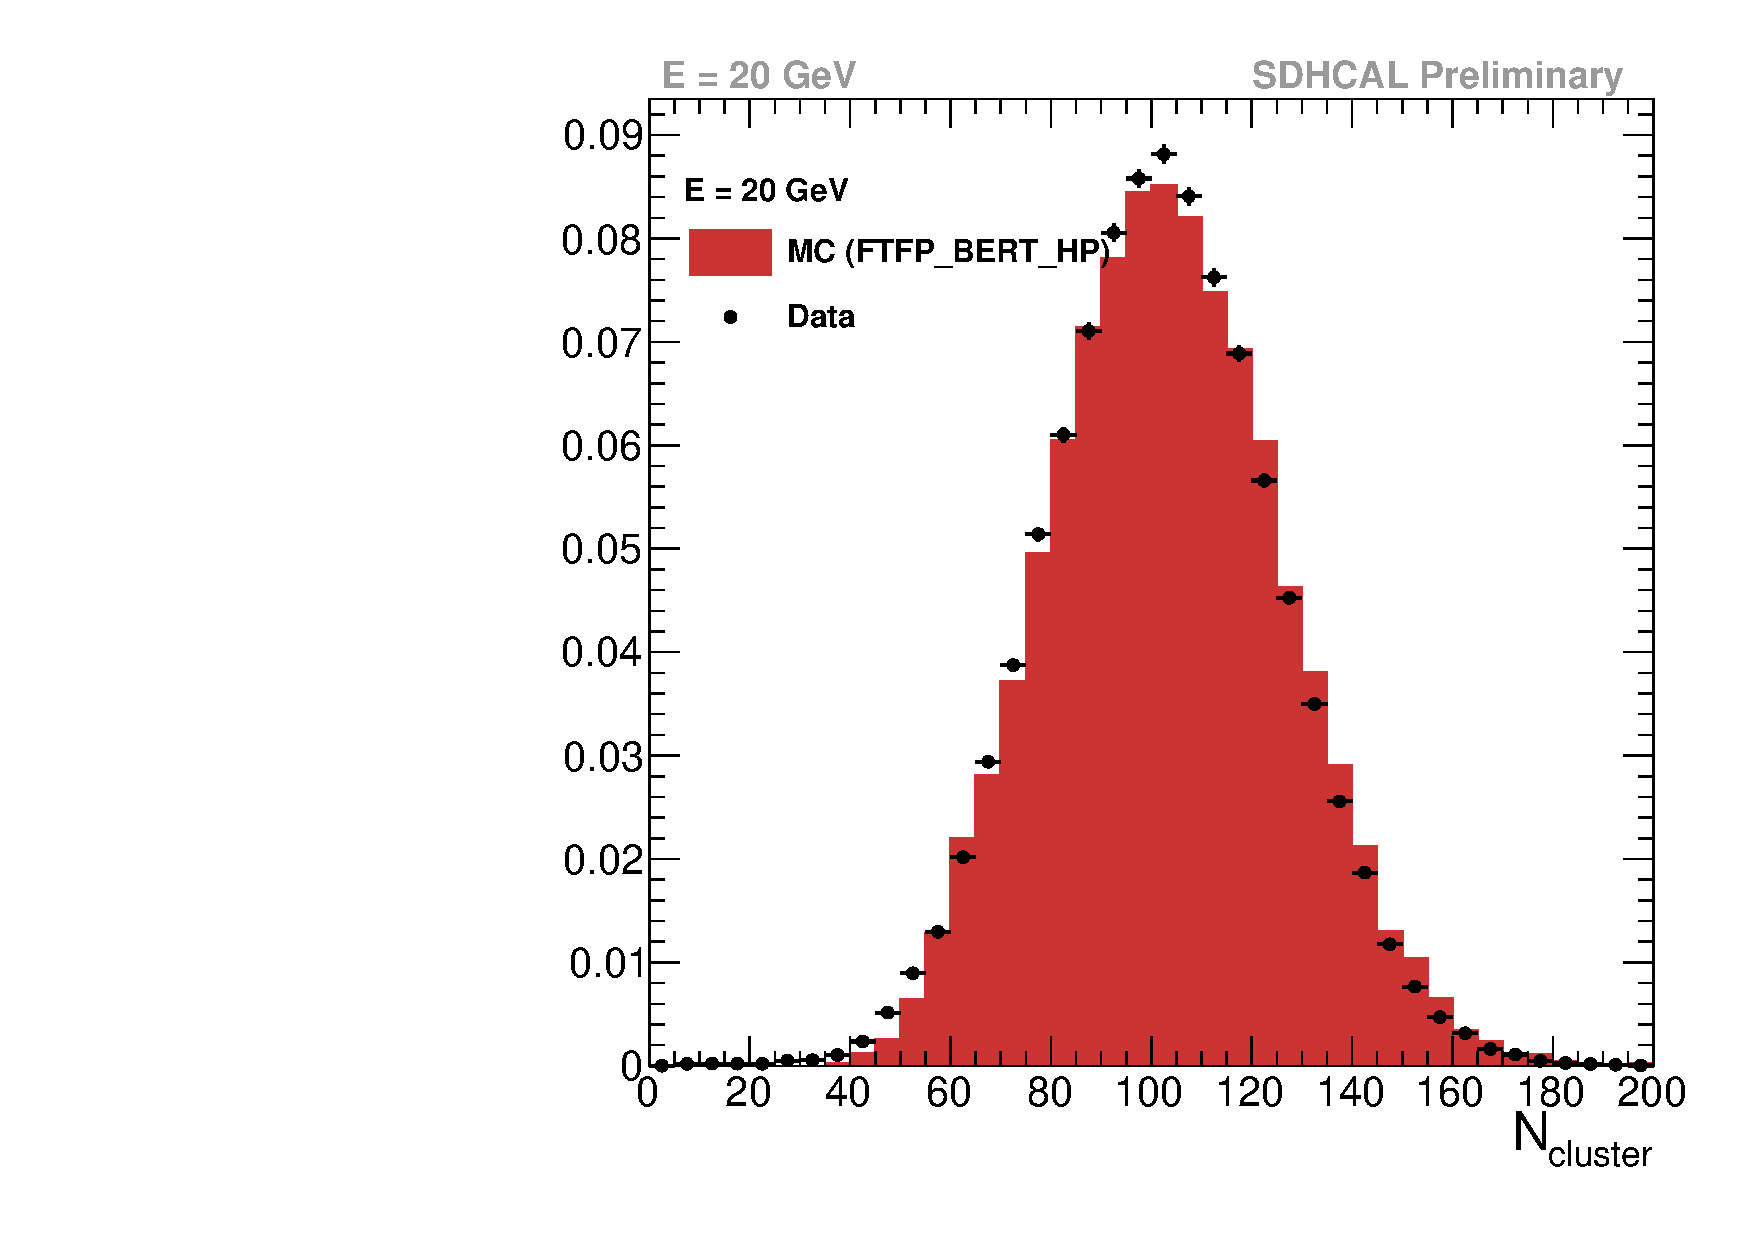
\includegraphics[width=.5\textwidth]{Shower/figs/ncluster_pi-_20GeV_AugSep2012.pdf}
  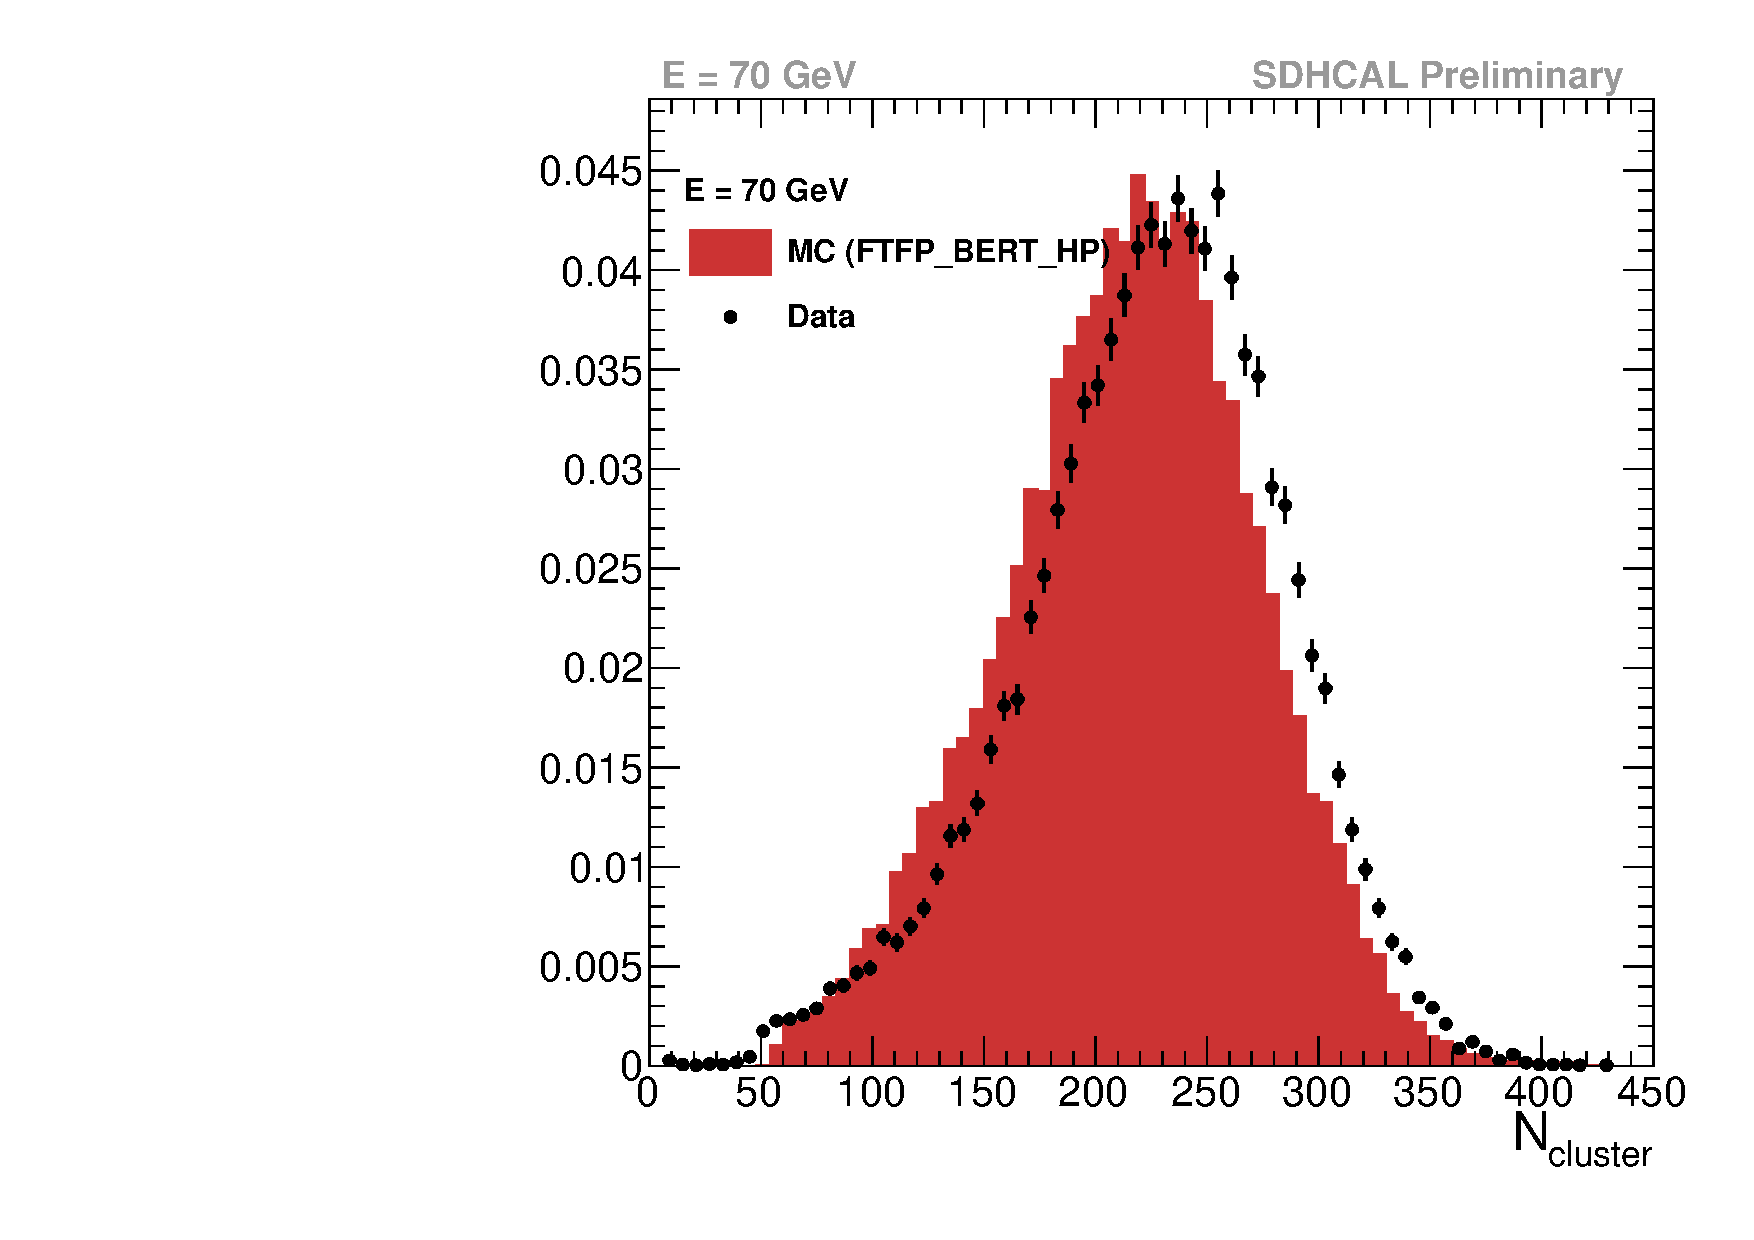
\includegraphics[width=.5\textwidth]{Shower/figs/ncluster_pi-_70GeV_AugSep2012.pdf}
  \caption{Distribution du nombre d'amas de hits pour des échantillons de pions de 20 (à gauche) et 70 (à droite) GeV. Les données sont représentées par des cercles noirs et la simulation (FTFP\_BERT\_HP) par les histogrammes rouges. \label{fig.pi-cluster}}
\end{figure}
La figure~\ref{fig.pi-cluster} présente les distributions du nombre d'amas de hits pour les données et la simulation (FTFP\_BERT\_HP) à 20 et 70 $GeV$. Comme pour le nombre total de hits, l'accord entre donnée et simulation est raisonnable à basse énergie et se dégrade à plus haute énergie.
\begin{figure}[!ht]
  \centering
  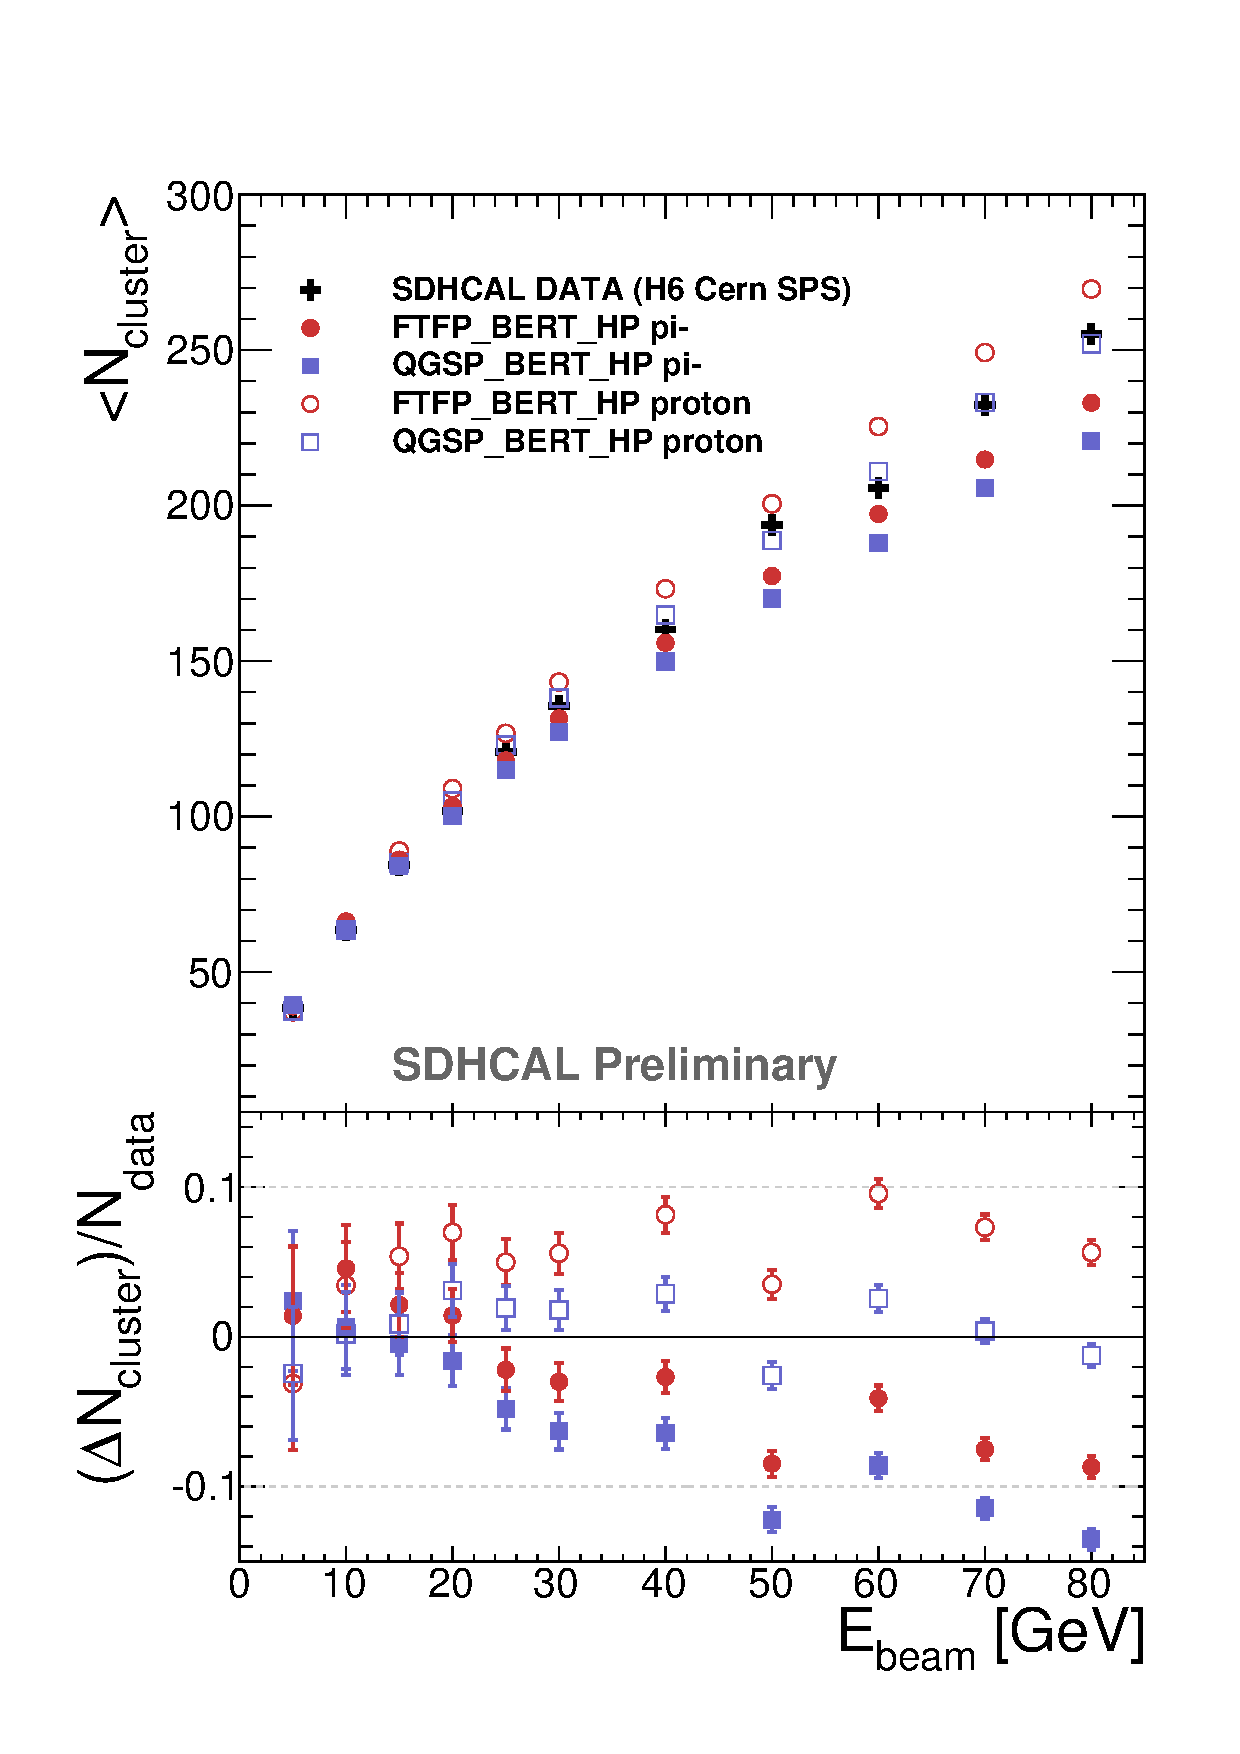
\includegraphics[width=.45\textwidth]{Shower/figs/NCLUSTERPIONHP.pdf}
  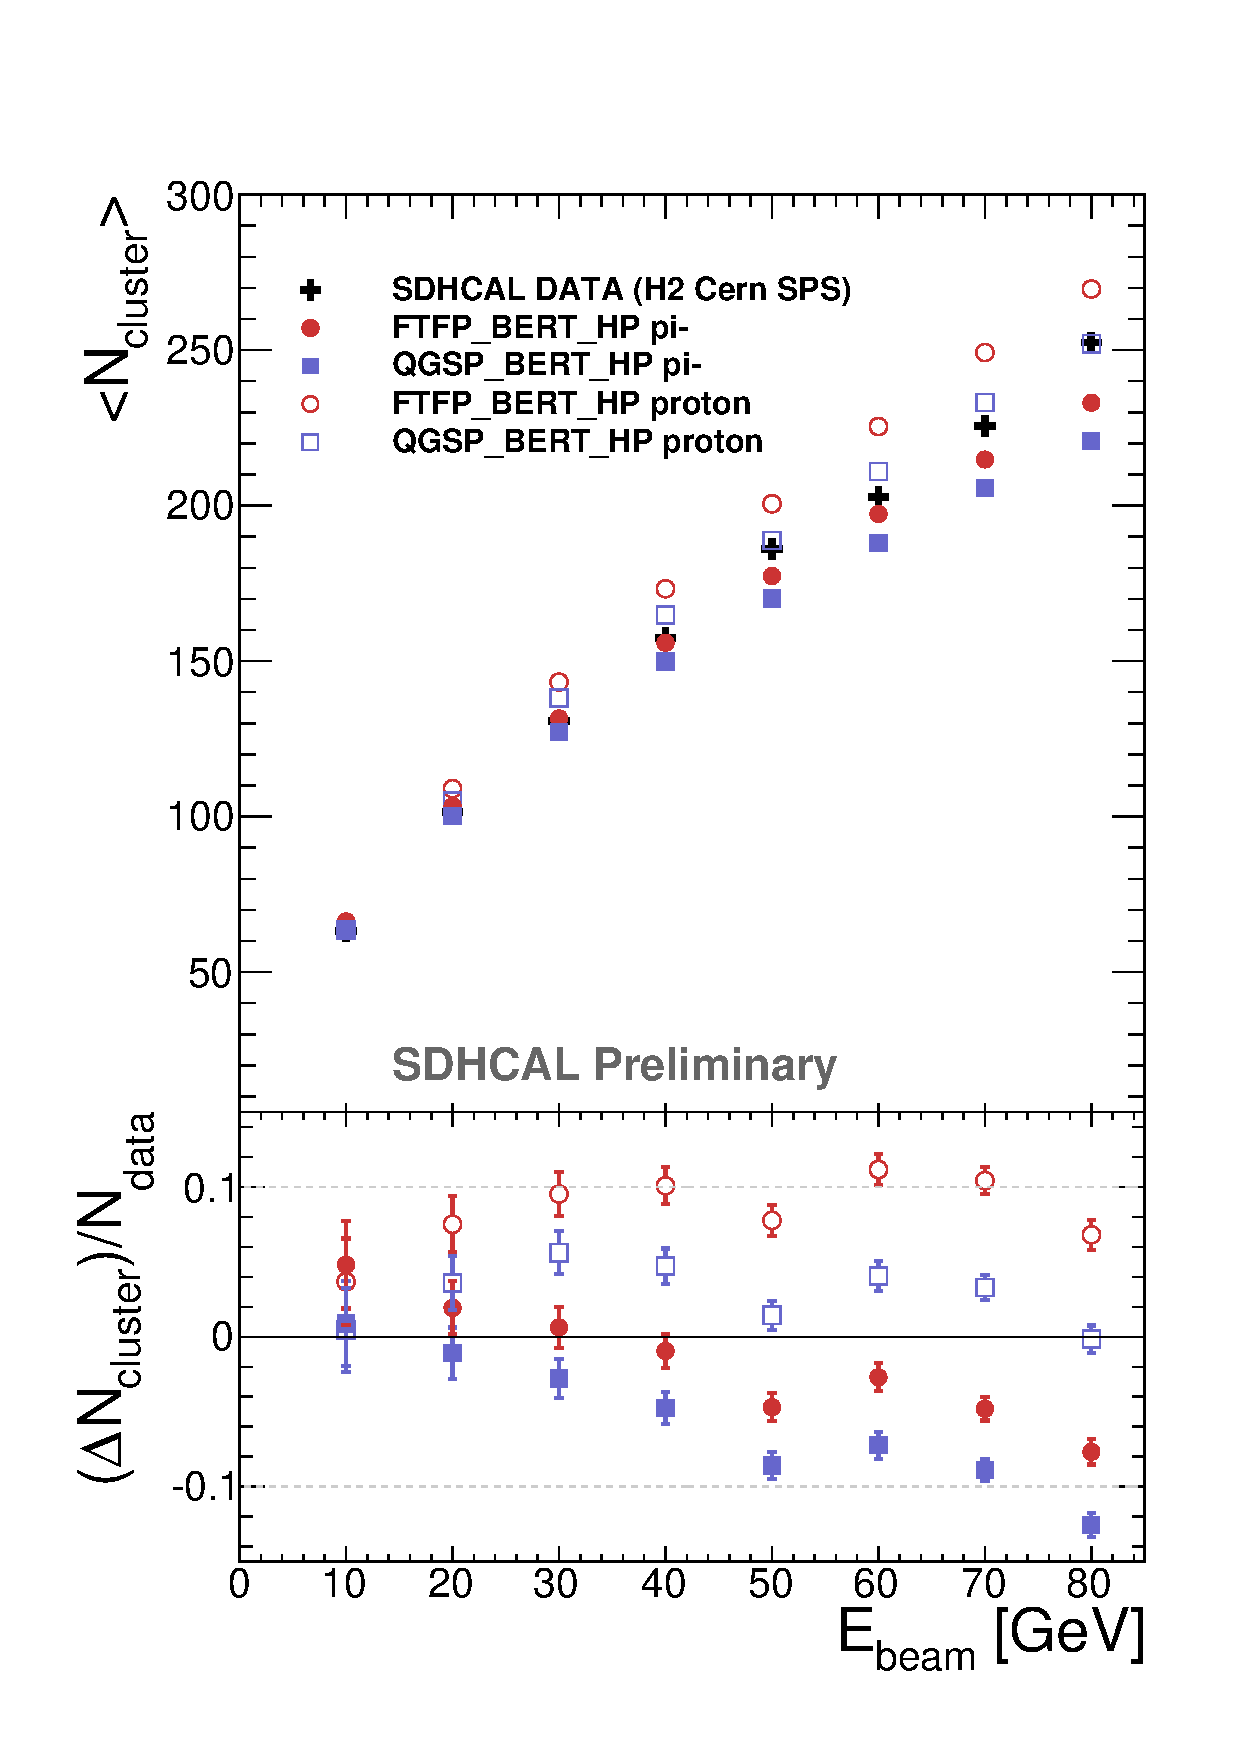
\includegraphics[width=.45\textwidth]{Shower/figs/NCLUSTERPIONNOV.pdf}
  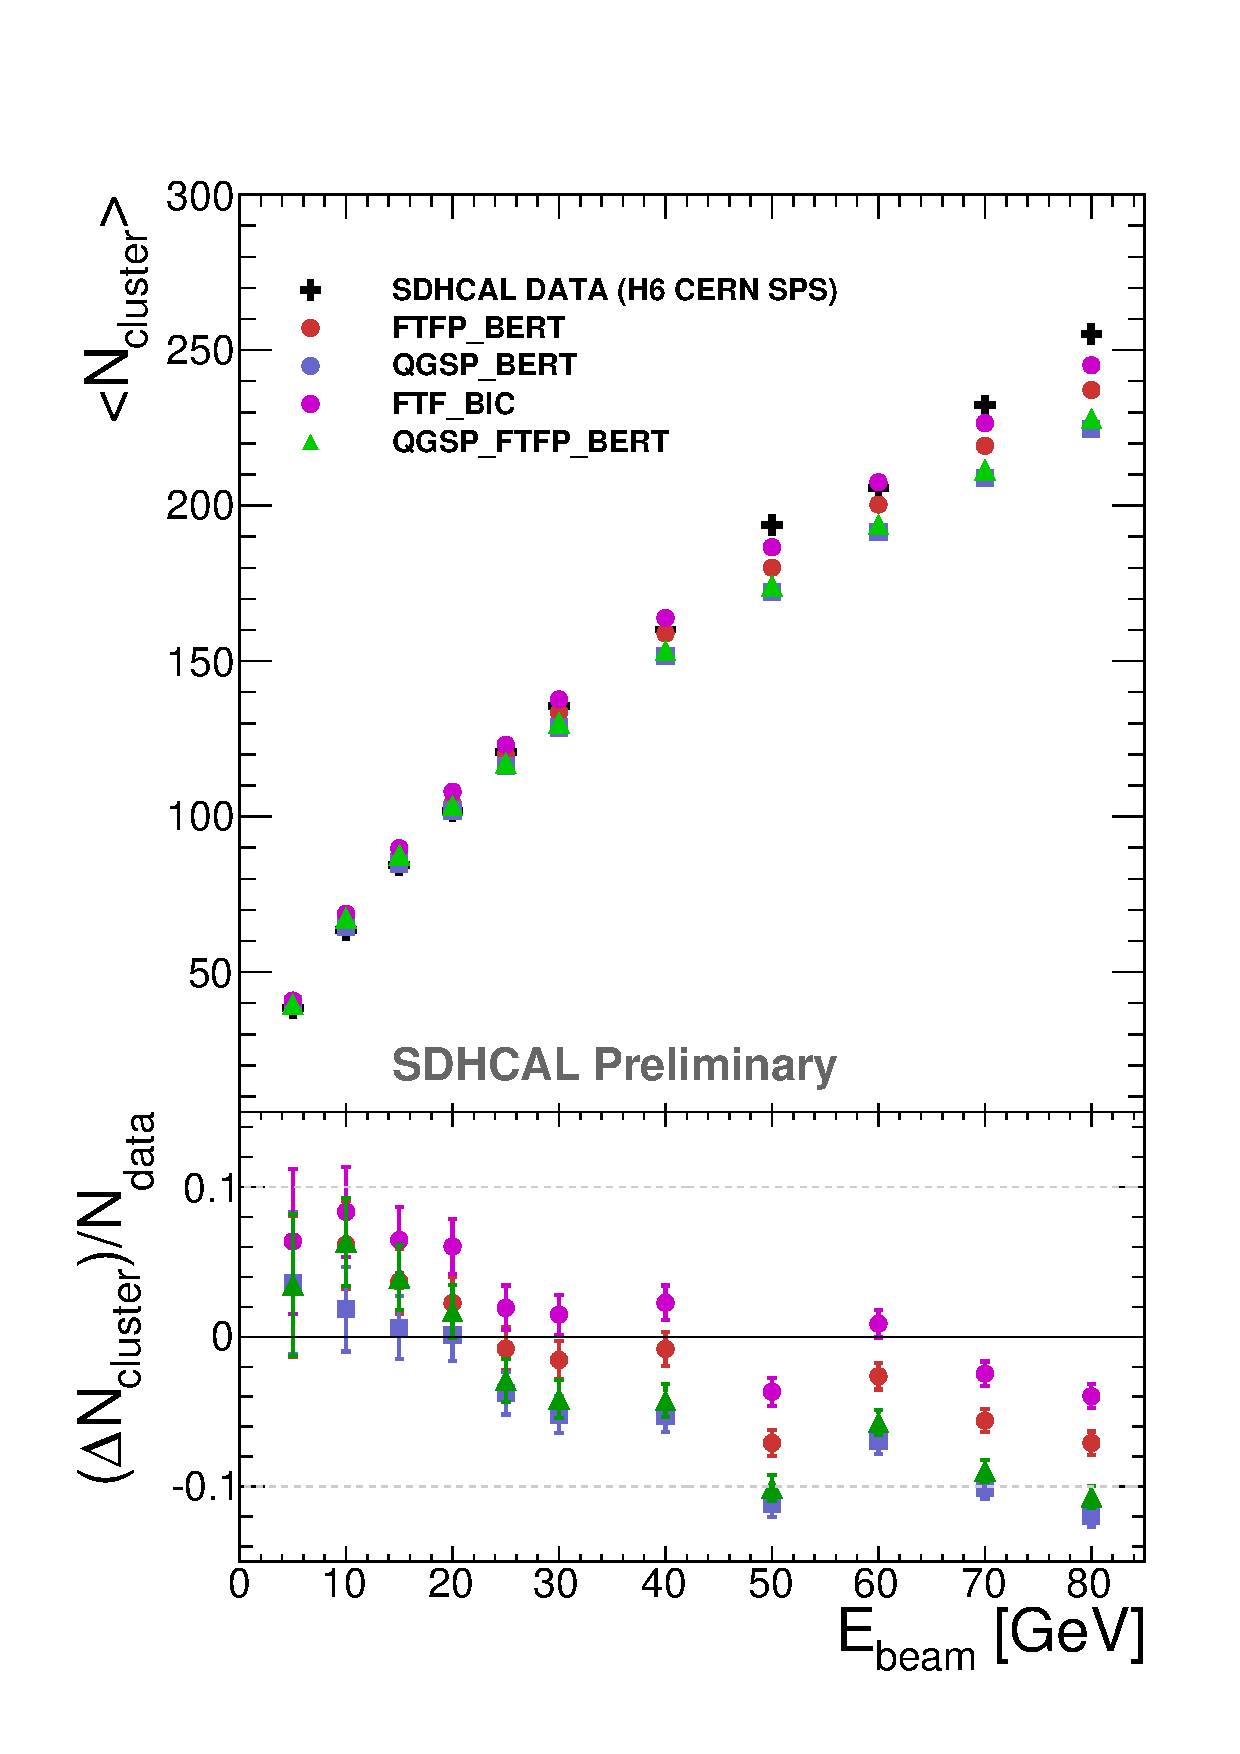
\includegraphics[width=.45\textwidth]{Shower/figs/NCLUSTERPION_MODEL.pdf}
  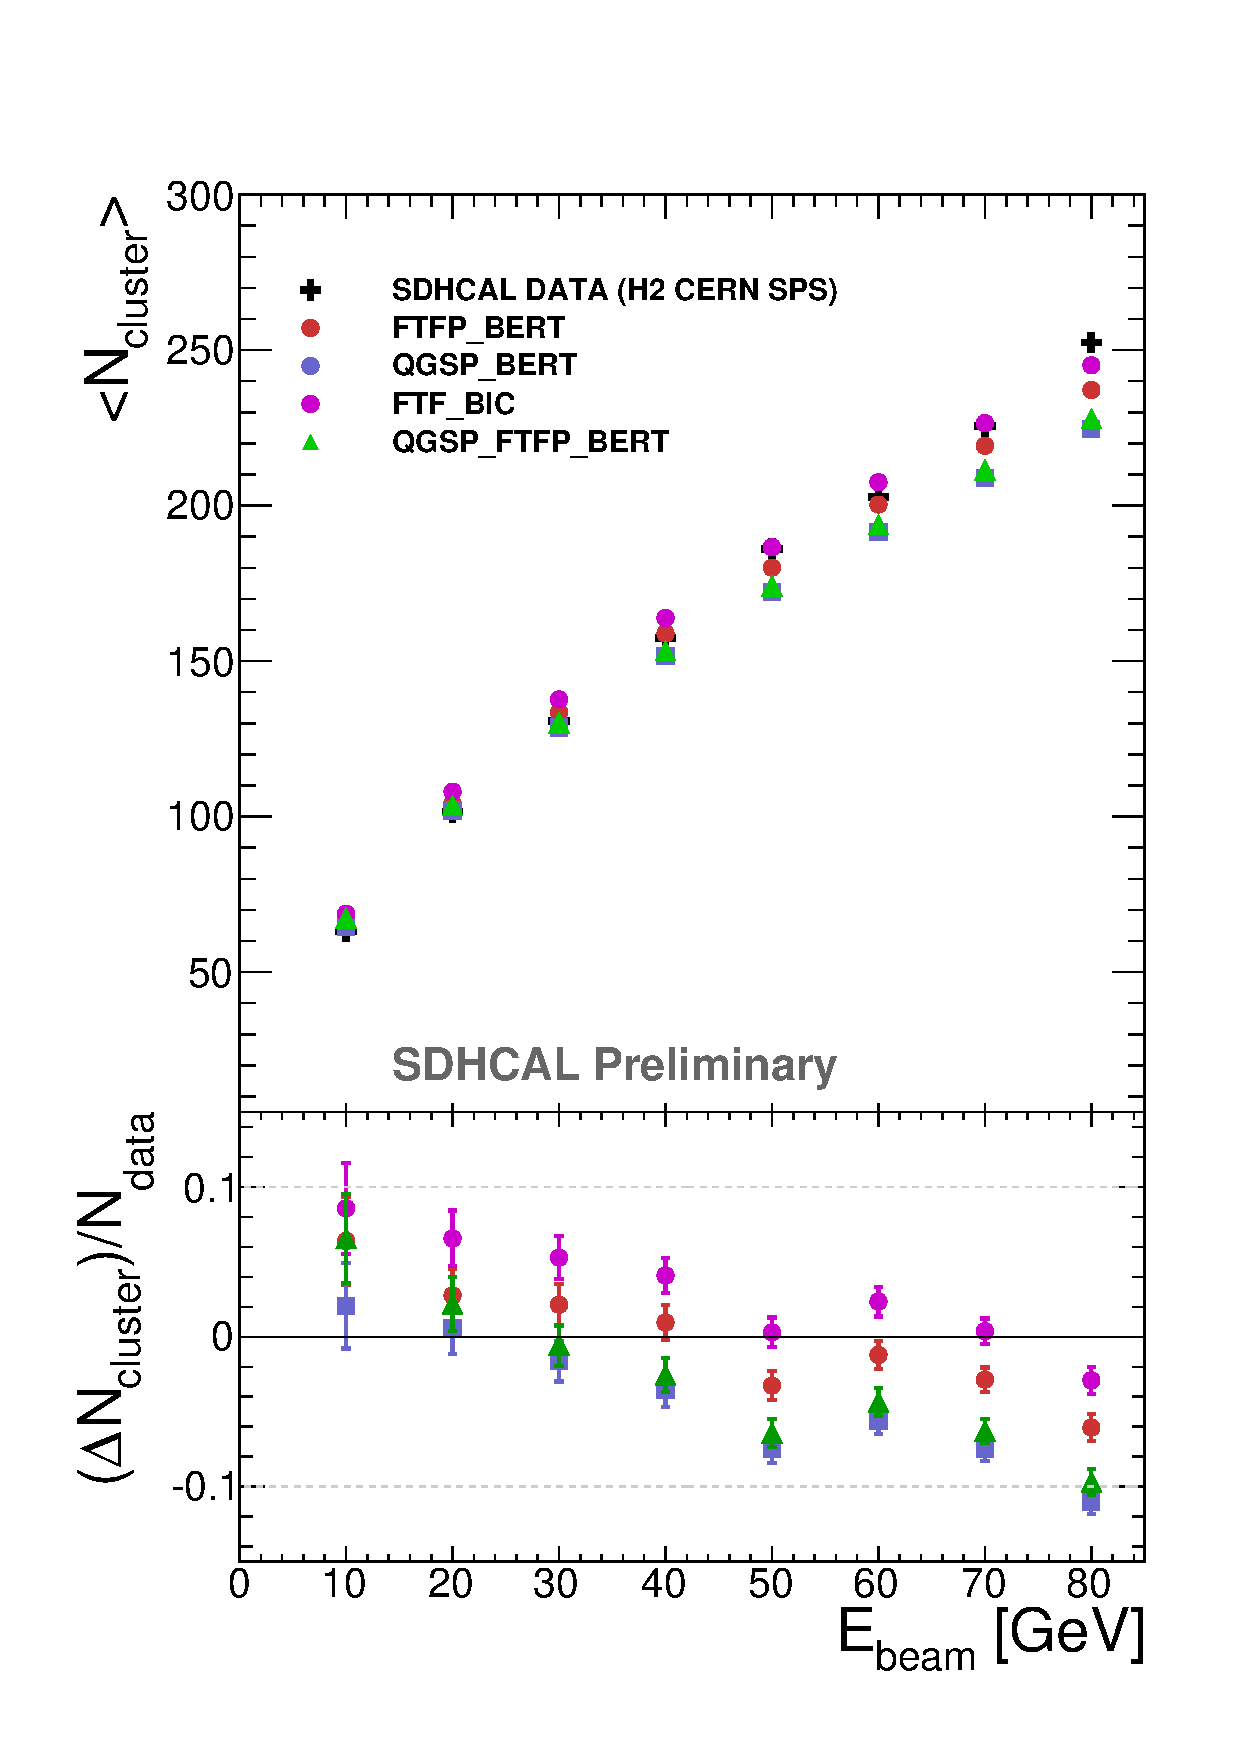
\includegraphics[width=.45\textwidth]{Shower/figs/NCLUSTERPION_MODEL_NOV.pdf}
  \caption{Nombre moyen d'amas de hits reconstruits pour des gerbes hadroniques en fonction de l'énergie du faisceau pour les données expérimentales et plusieurs listes physiques. Les déviations relatives sont aussi présentées. Les figures de gauche présentent les résultats avec les données de la ligne H6 et les figures de droite avec les données de la ligne H2 du CERN.}
  \label{fig.cluster_pi-_ebeam}
\end{figure}
La figure~\ref{fig.cluster_pi-_ebeam} montre le nombre moyen d'amas de hits en fonction de l'énergie du faisceau pour les données et plusieurs listes physiques. Les déviations relatives définies par $\frac{<N_{simu}>-<N_{data}>}{<N_{data}>}$, où $<N_{data}>$ et $<N_{simu}>$ sont respectivement les nombres moyens d'amas pour les données et la simulation, sont indiquées. Le nombre de hits de bruits, estimé à 1.75 par événement physique (cf. section~\ref{sec.trivent} du chapitre~\ref{chap.sdhcal}) est inclus dans les barres d'erreurs. Pour du bruit incohérent, le nombre d'amas résultants est à priori le même que le nombre de cellules touchées dues au bruit. 

La figure~\ref{fig.cluster_pi-_ebeam} montre des différences significatives sur le nombre d'amas entre les gerbes hadroniques initiées par des protons et celles initiées par des pions. Ces différences s’expliquent par la fraction électromagnétique plus faible dans les cascades initiées par des protons (cf. section~\ref{sec.fem} du chapitre~\ref{chap.shower}). De plus, la longueur d'interaction des protons est plus faible que celle des pions. Ainsi, la quantité d'énergie s'échappant du détecteur est plus faible dans les cascades initiées par des protons que pour celles initiées par des pions. L'utilisation de l'option de haute précision pour les neutrons fait légèrement diminuer le nombre d'amas reconstruits. La plupart des listes sous-estiment le nombre d'amas reconstruits. Ceci confirme les observations sur le nombre de cellules touchées dans le chapitre précédent. La liste FTF\_BIC est, comme pour le nombre total de cellules touchées, la plus proche des données expérimentales à haute énergie mais surestime légèrement le nombre d'amas en dessous de 40 $GeV$. 

\begin{figure}[!ht]
  \subfigure[]{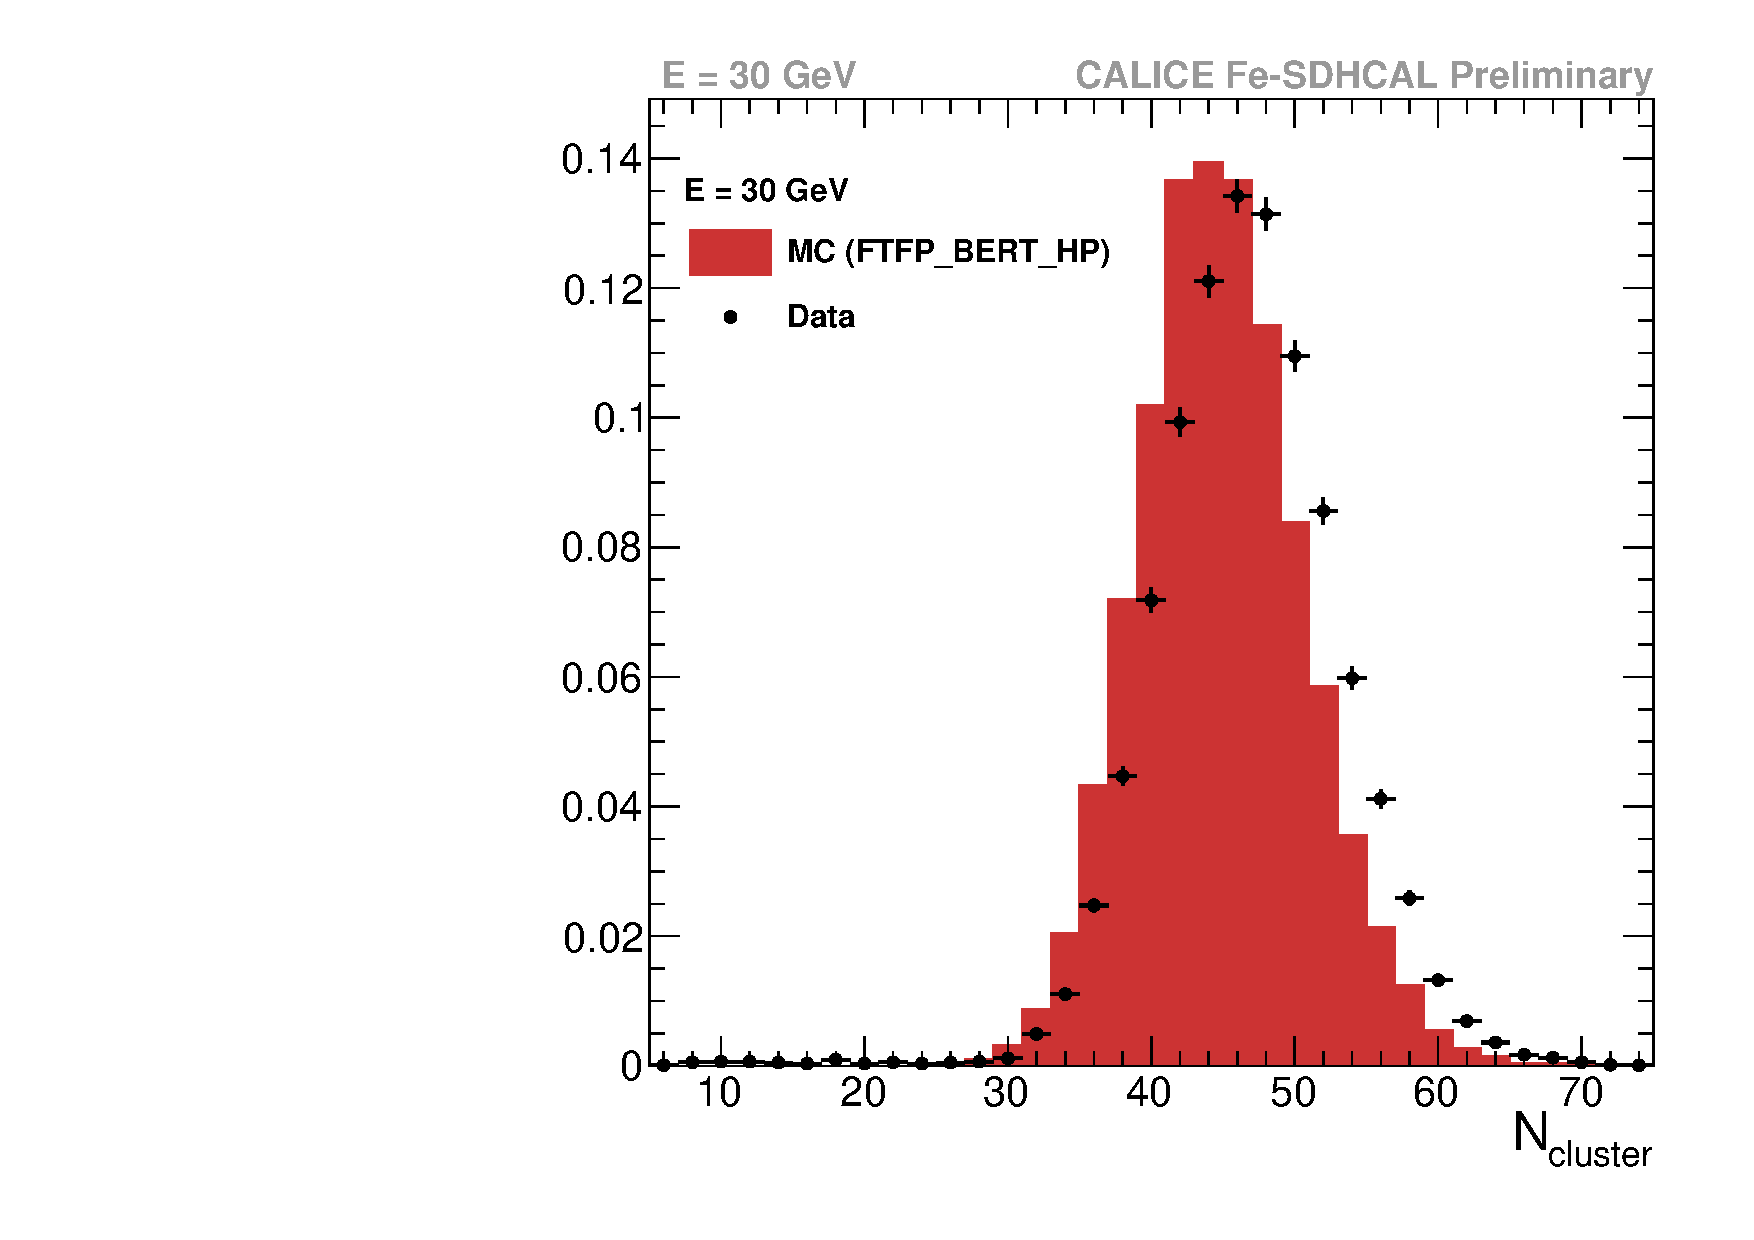
\includegraphics[width=.5\textwidth]{Shower/figs/ncluster_e-_30GeV_AugSep2012.pdf}}
  \subfigure[]{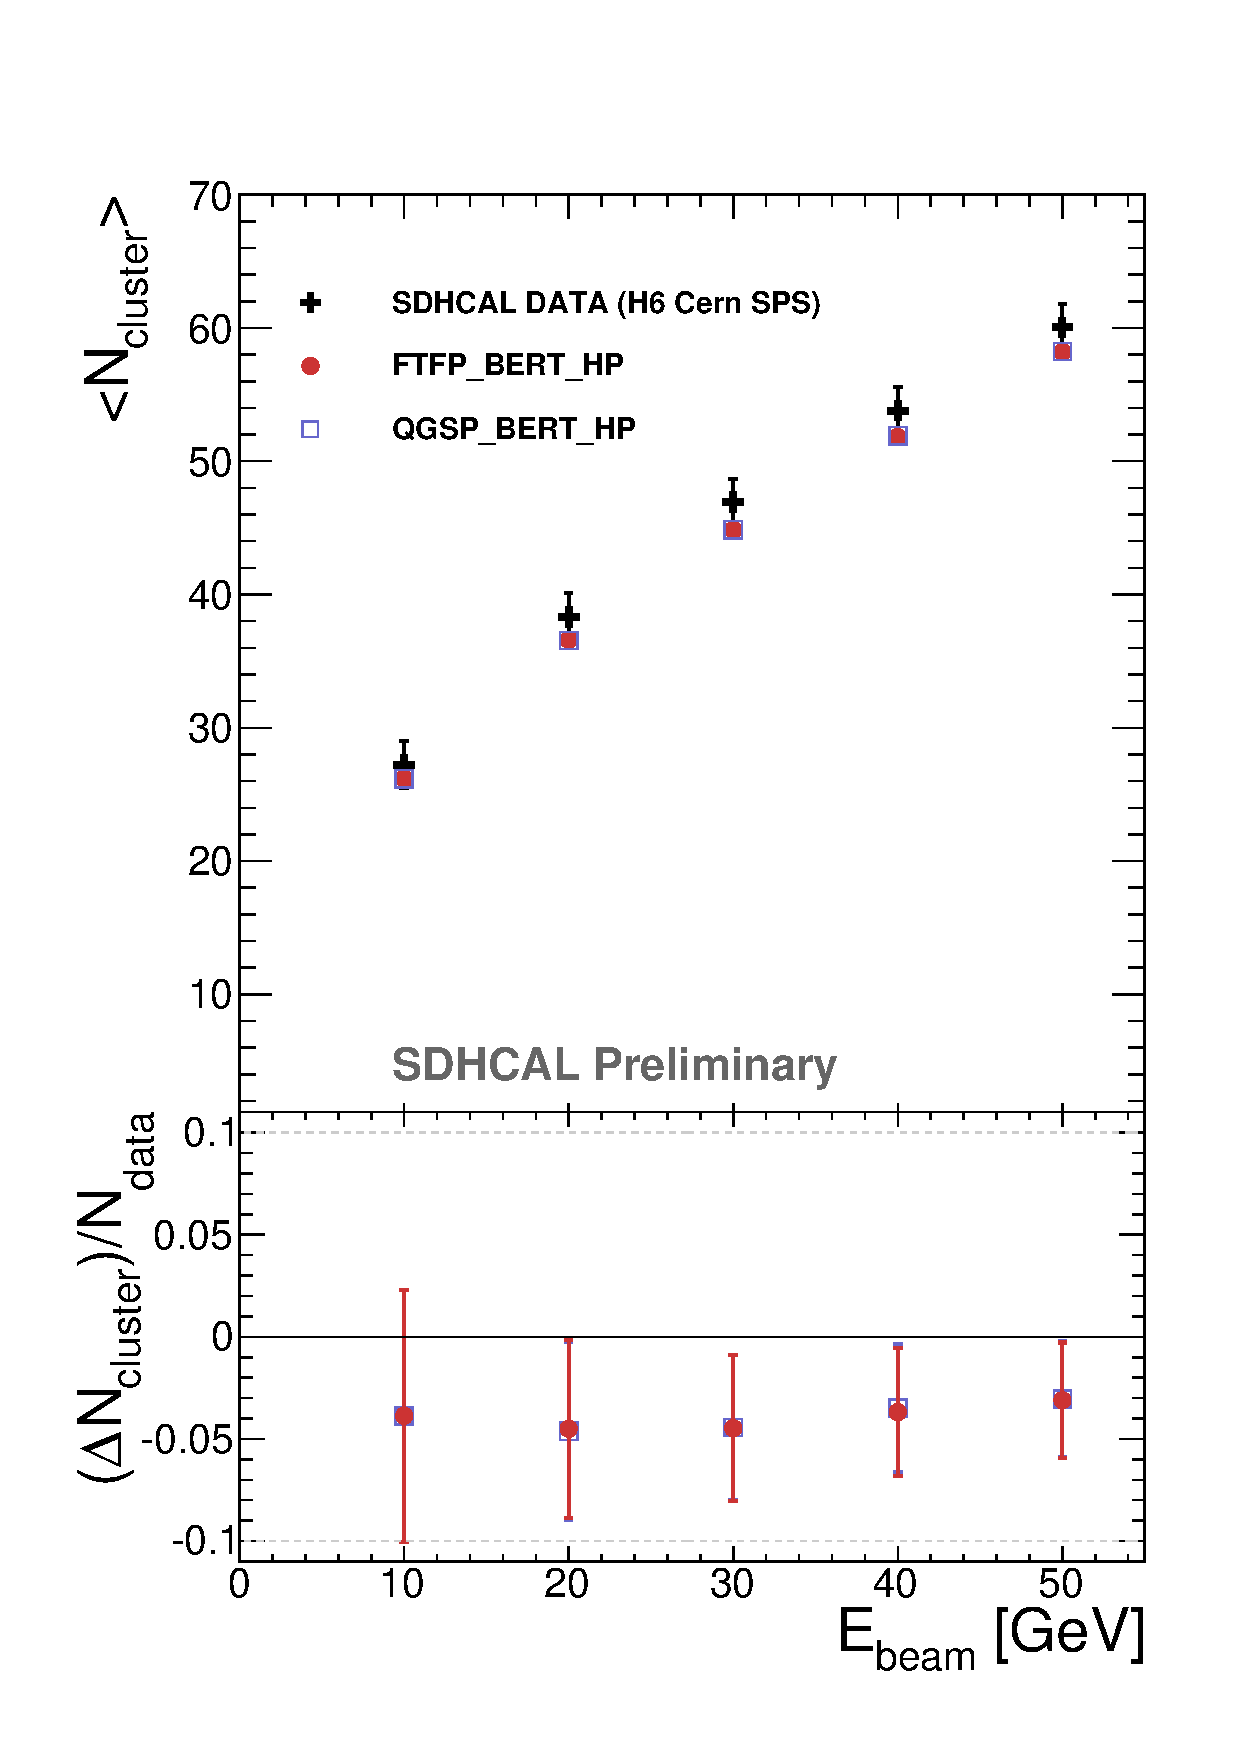
\includegraphics[width=.4\textwidth]{Shower/figs/NCLUSTERELECTRON.pdf}}
  \caption{(a): Distribution du nombre d'amas de hits dans les gerbes électromagnétiques de 30 $GeV$ pour les données (cercles noirs) et la simulation (histogramme rouge). (b) Nombre moyen d'amas de hits reconstruits et déviation relative pour des gerbes électromagnétiques en fonction de l'énergie du faisceau.}
  \label{fig.cluster_e-}
\end{figure}
Les amas de hits sont aussi étudiés pour les gerbes électromagnétiques. La figure~\ref{fig.cluster_e-}(a) montre la distribution du nombre d'amas de hits pour des gerbes électromagnétiques de 30 $GeV$ pour les données et la simulation. La figure~\ref{fig.cluster_e-}(b) montre le nombre moyen d'amas de hits reconstruits en fonction de l'énergie pour des gerbes électromagnétiques. La simulation sous-estime très légèrement le nombre d'amas par rapport aux données. La déviation relative est inférieure à 5$\%$ sur toute la gamme d'énergie. La différence des nombres moyens d'amas reconstruits entre la simulation et les données est inférieure à 2 sur toute la gamme d'énergie. Cette différence vient probablement du bruit dans le prototype, estimé à environ 1.75 hits par événement physique (cf. section~\ref{sec.trivent} du chapitre~\ref{chap.sdhcal}). %Les gerbes hadroniques identifiées comme électromagnétiques peuvent aussi contribuer à la différence observée. Le nombre de groupes de ces cascades a aussi été étudié avec la simulation. La déviation relative entre ces événements de simulation et les données et de l'ordre de 40$\%$ sur toute la gamme d'énergie. 

%%%%%%%%%%%%%%%%%%%%%%%%%%%%%%%%%%%%%%%%%%%%%%%
\newpage
\section{Les profils des gerbes hadroniques}
\label{sec.Profil}
\subsection{Profil longitudinal}
\label{sec.longiProfil}
\begin{figure}[!ht]
  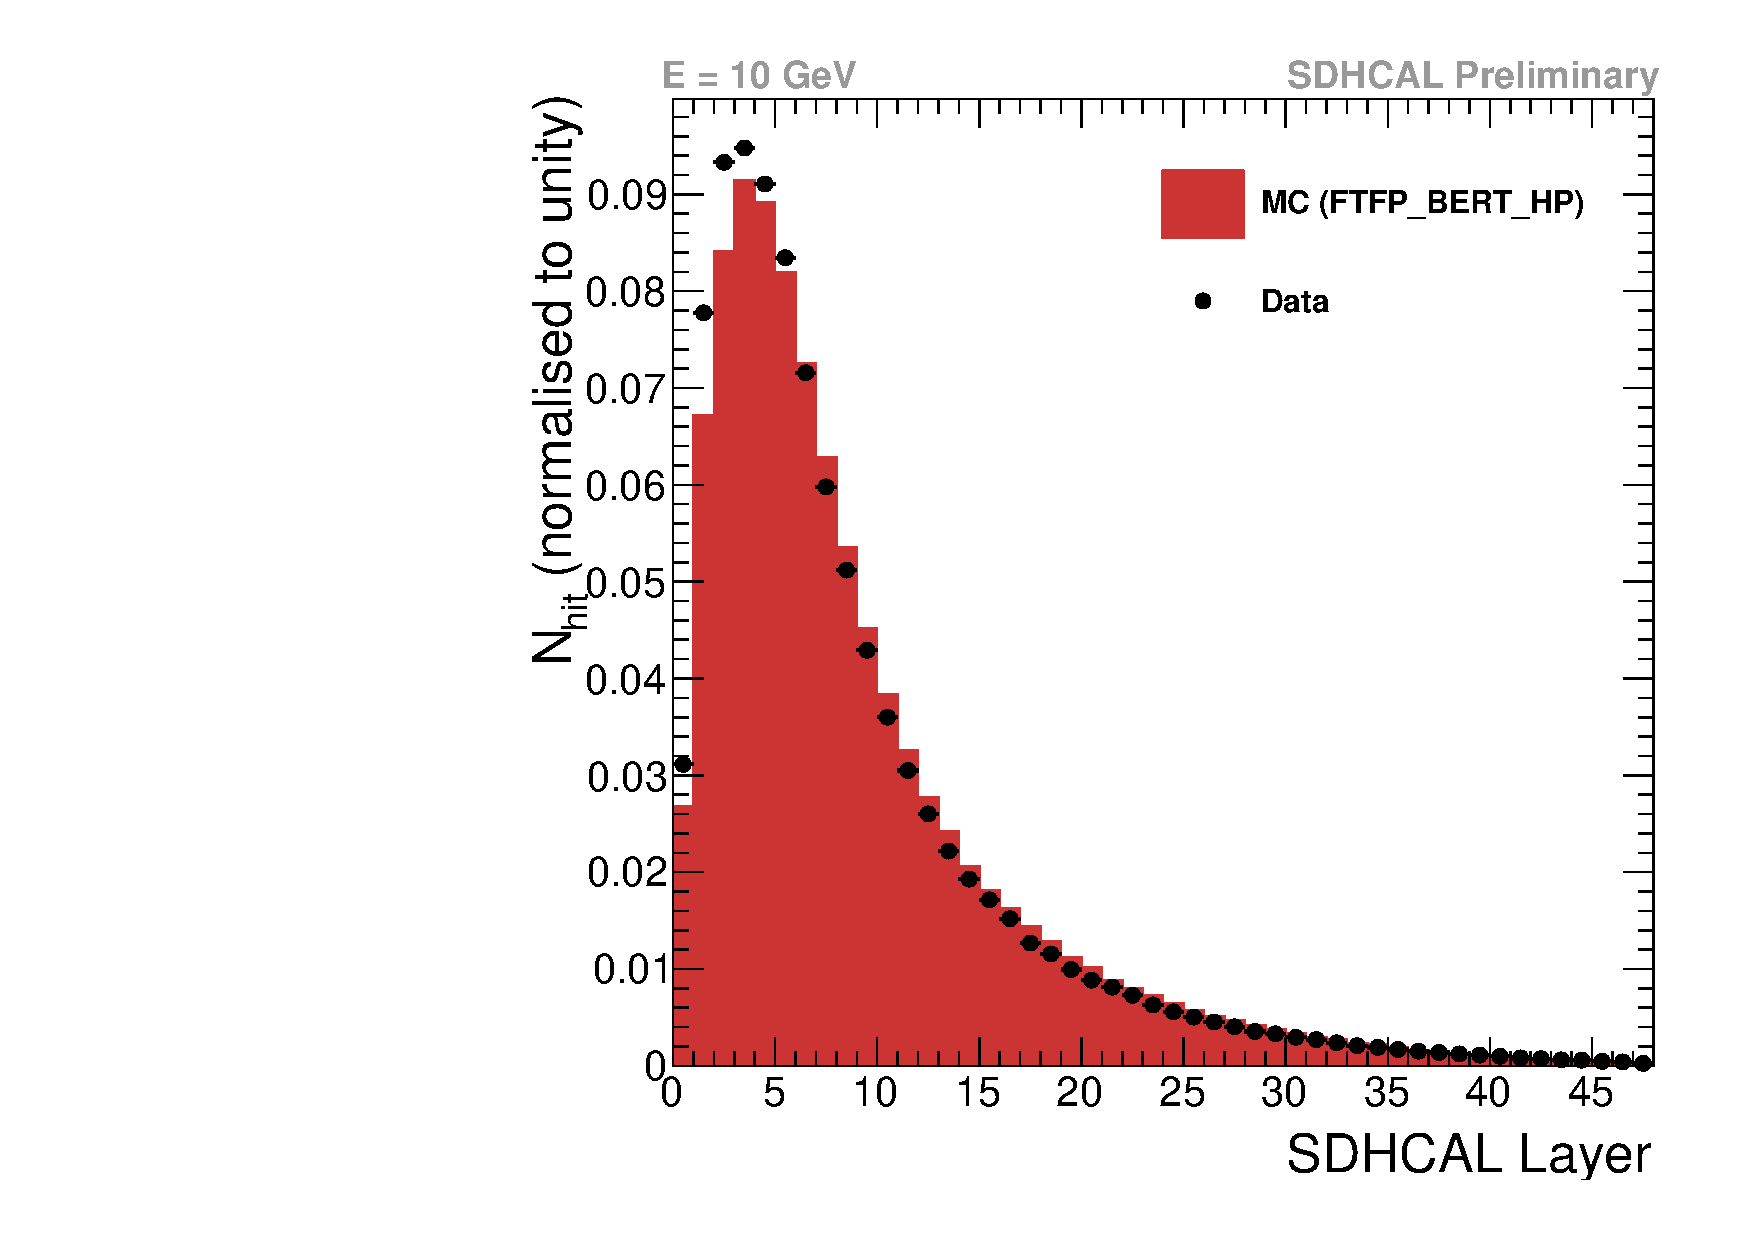
\includegraphics[width=.32\textwidth]{Shower/figs/longiProf_pi-_10GeV_ftfp_bert_hp.pdf}
  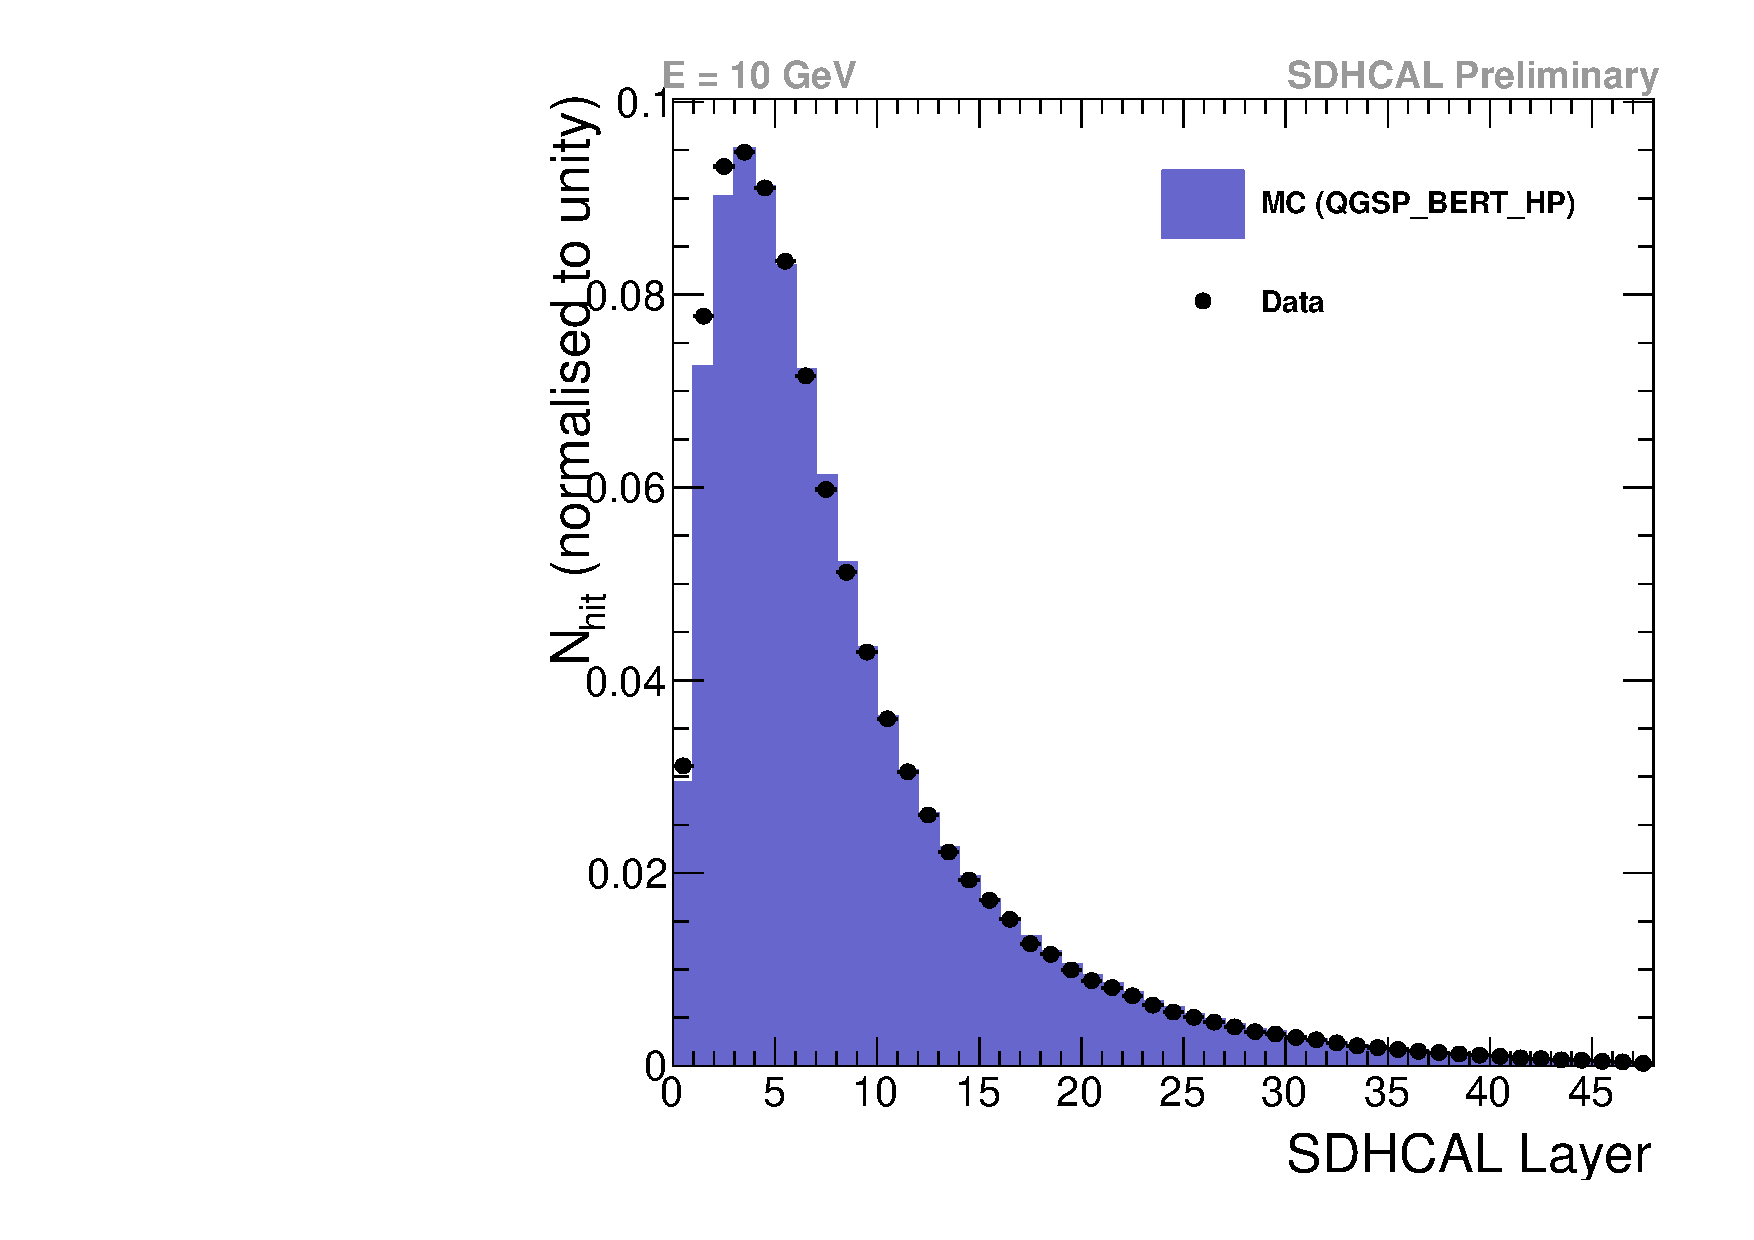
\includegraphics[width=.32\textwidth]{Shower/figs/longiProf_pi-_10GeV_qgsp_bert_hp.pdf}
  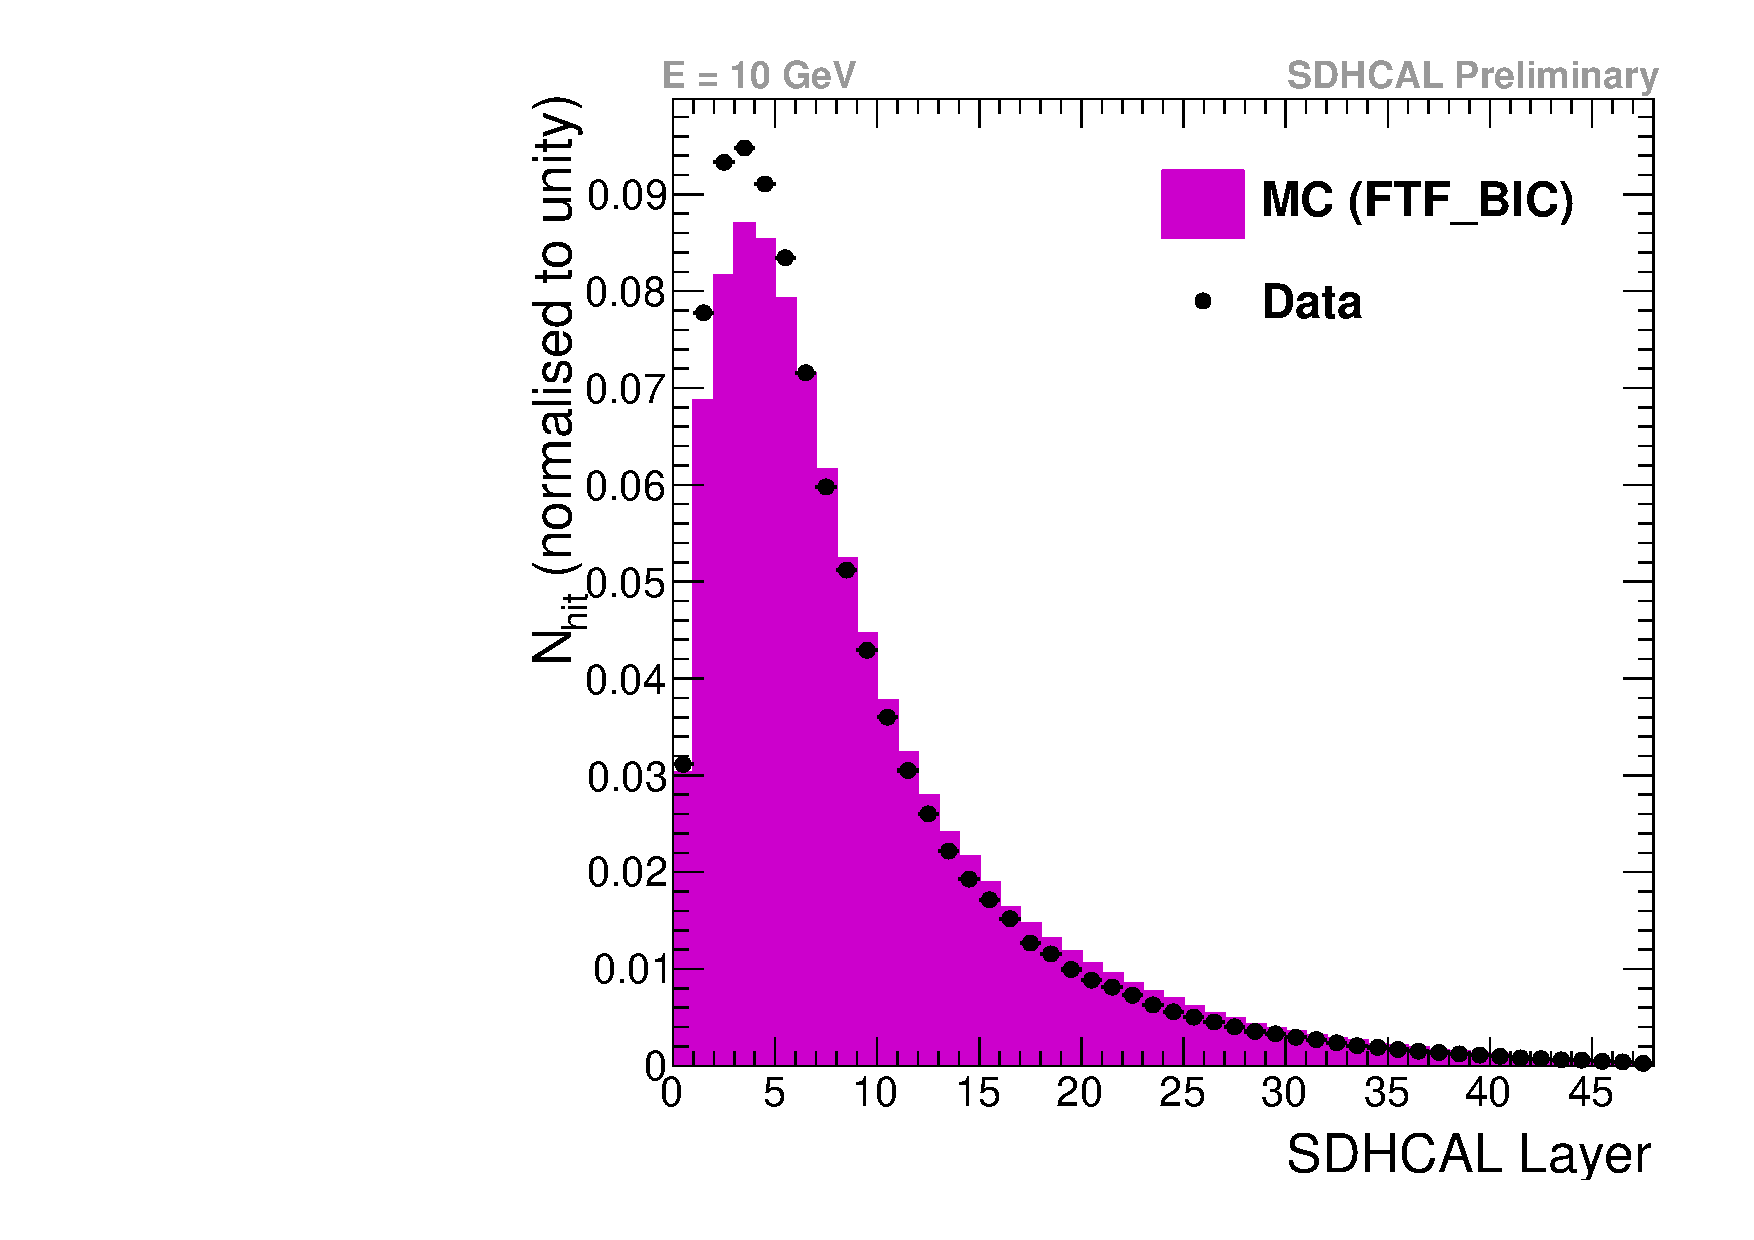
\includegraphics[width=.32\textwidth]{Shower/figs/longiProf_pi-_10GeV_ftf_bic.pdf}\\
  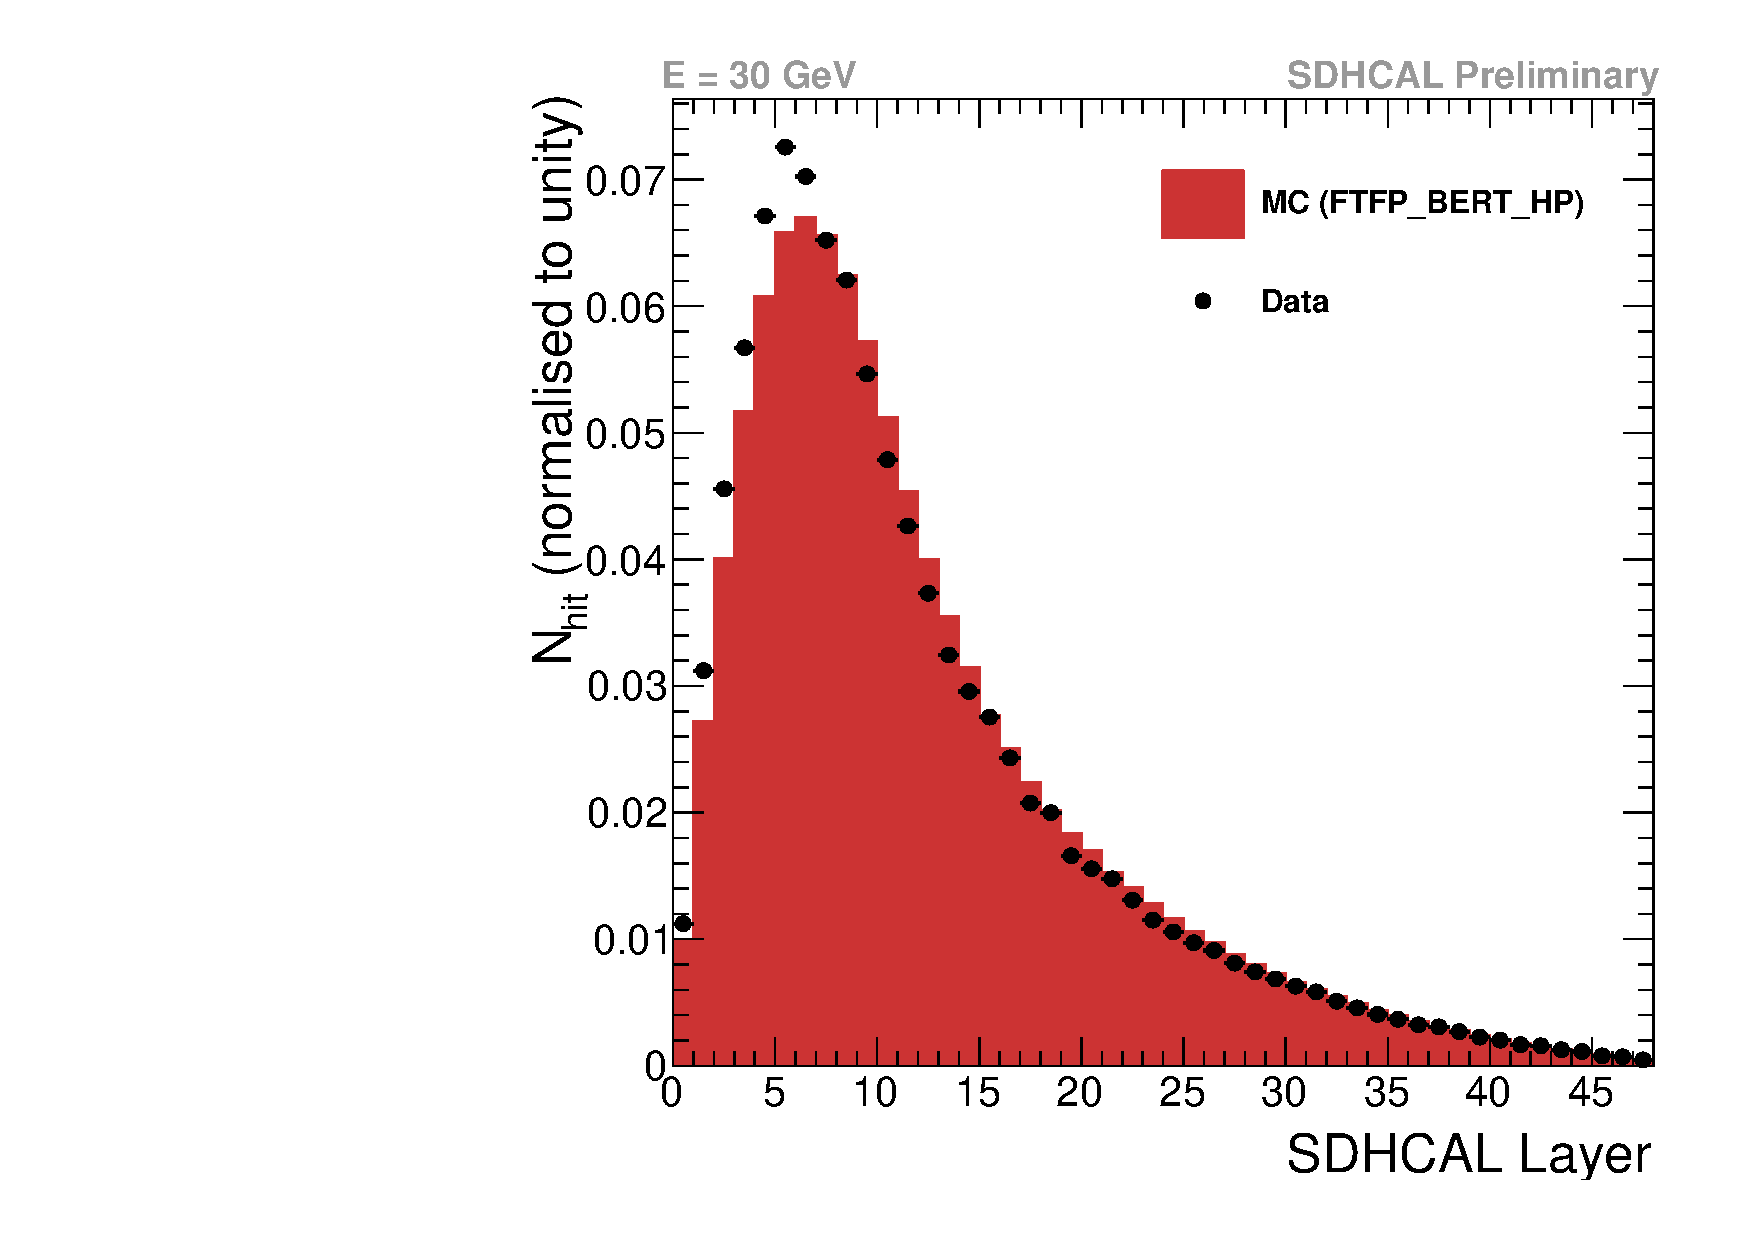
\includegraphics[width=.32\textwidth]{Shower/figs/longiProf_pi-_30GeV_ftfp_bert_hp.pdf}
  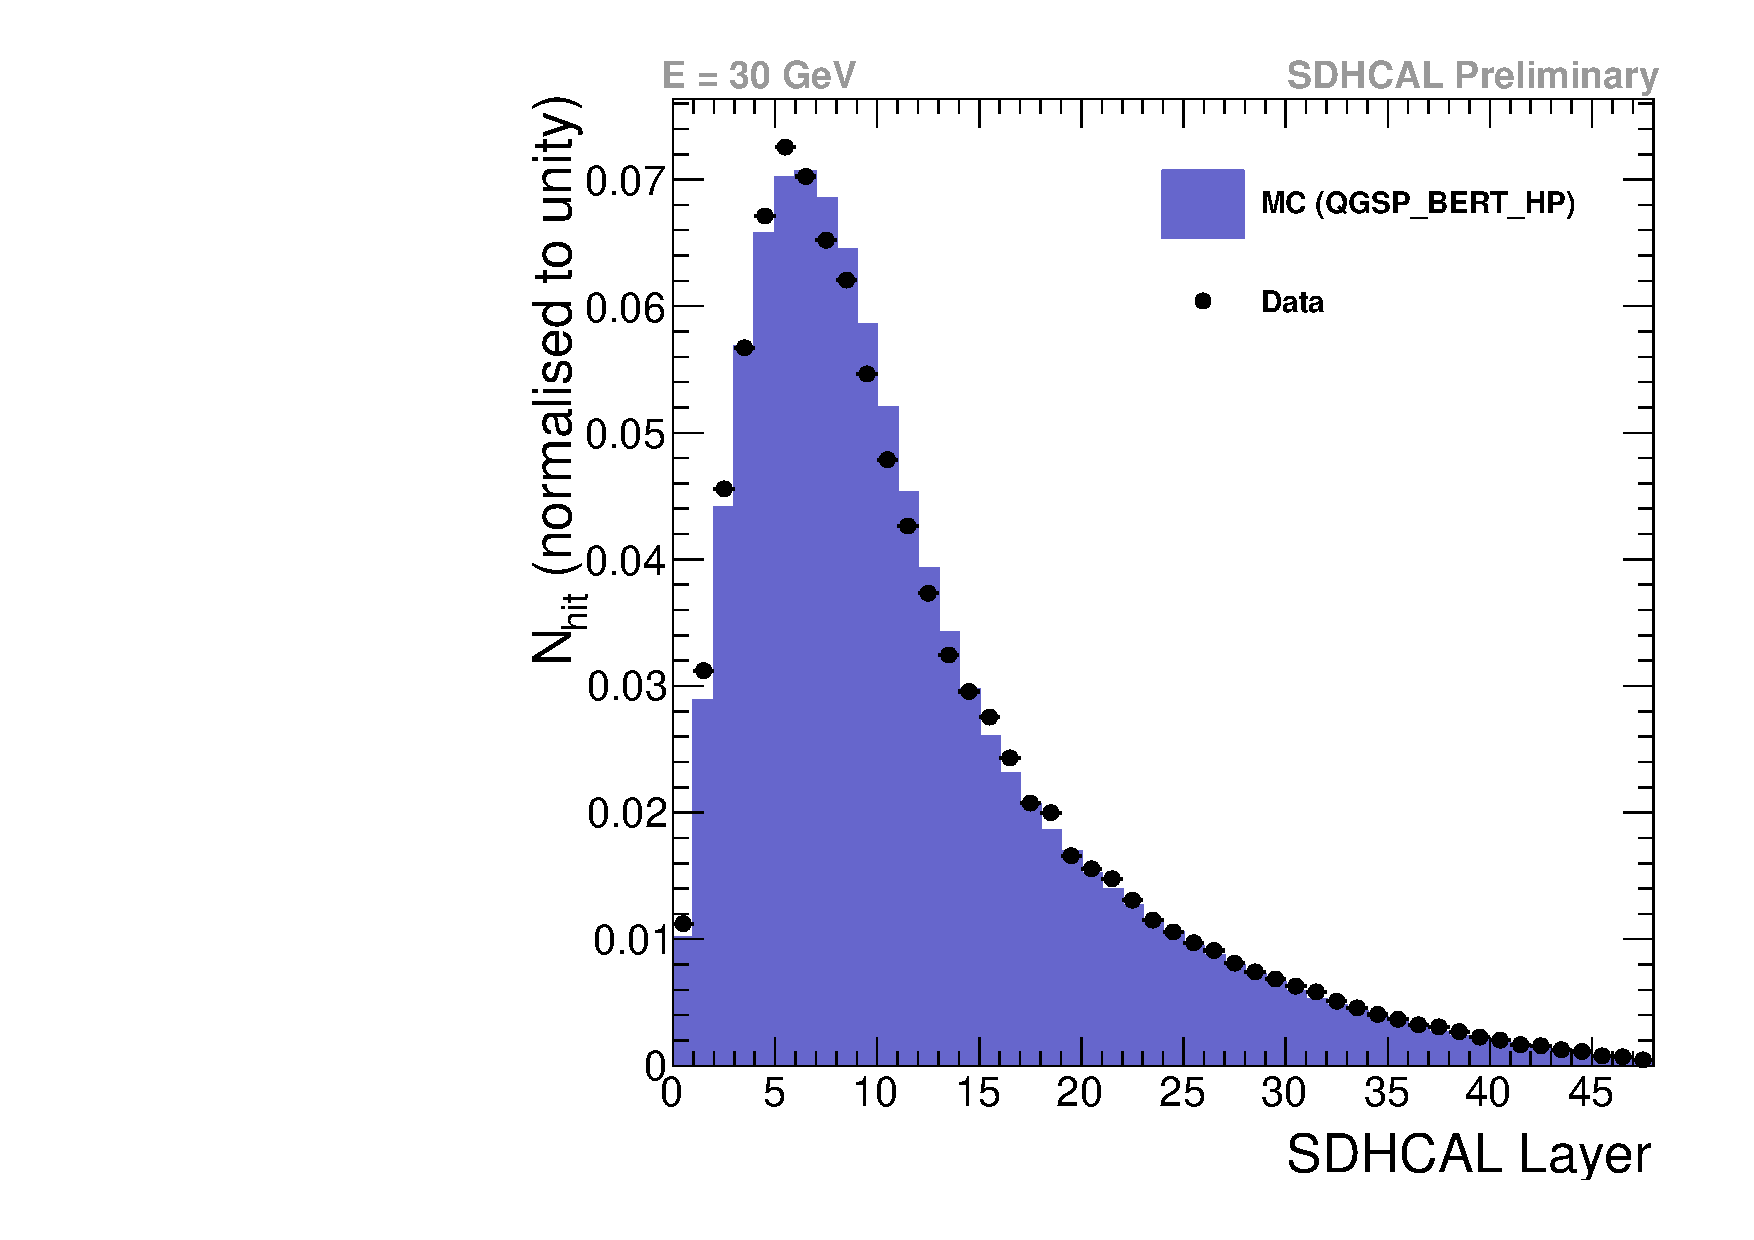
\includegraphics[width=.32\textwidth]{Shower/figs/longiProf_pi-_30GeV_qgsp_bert_hp.pdf}
  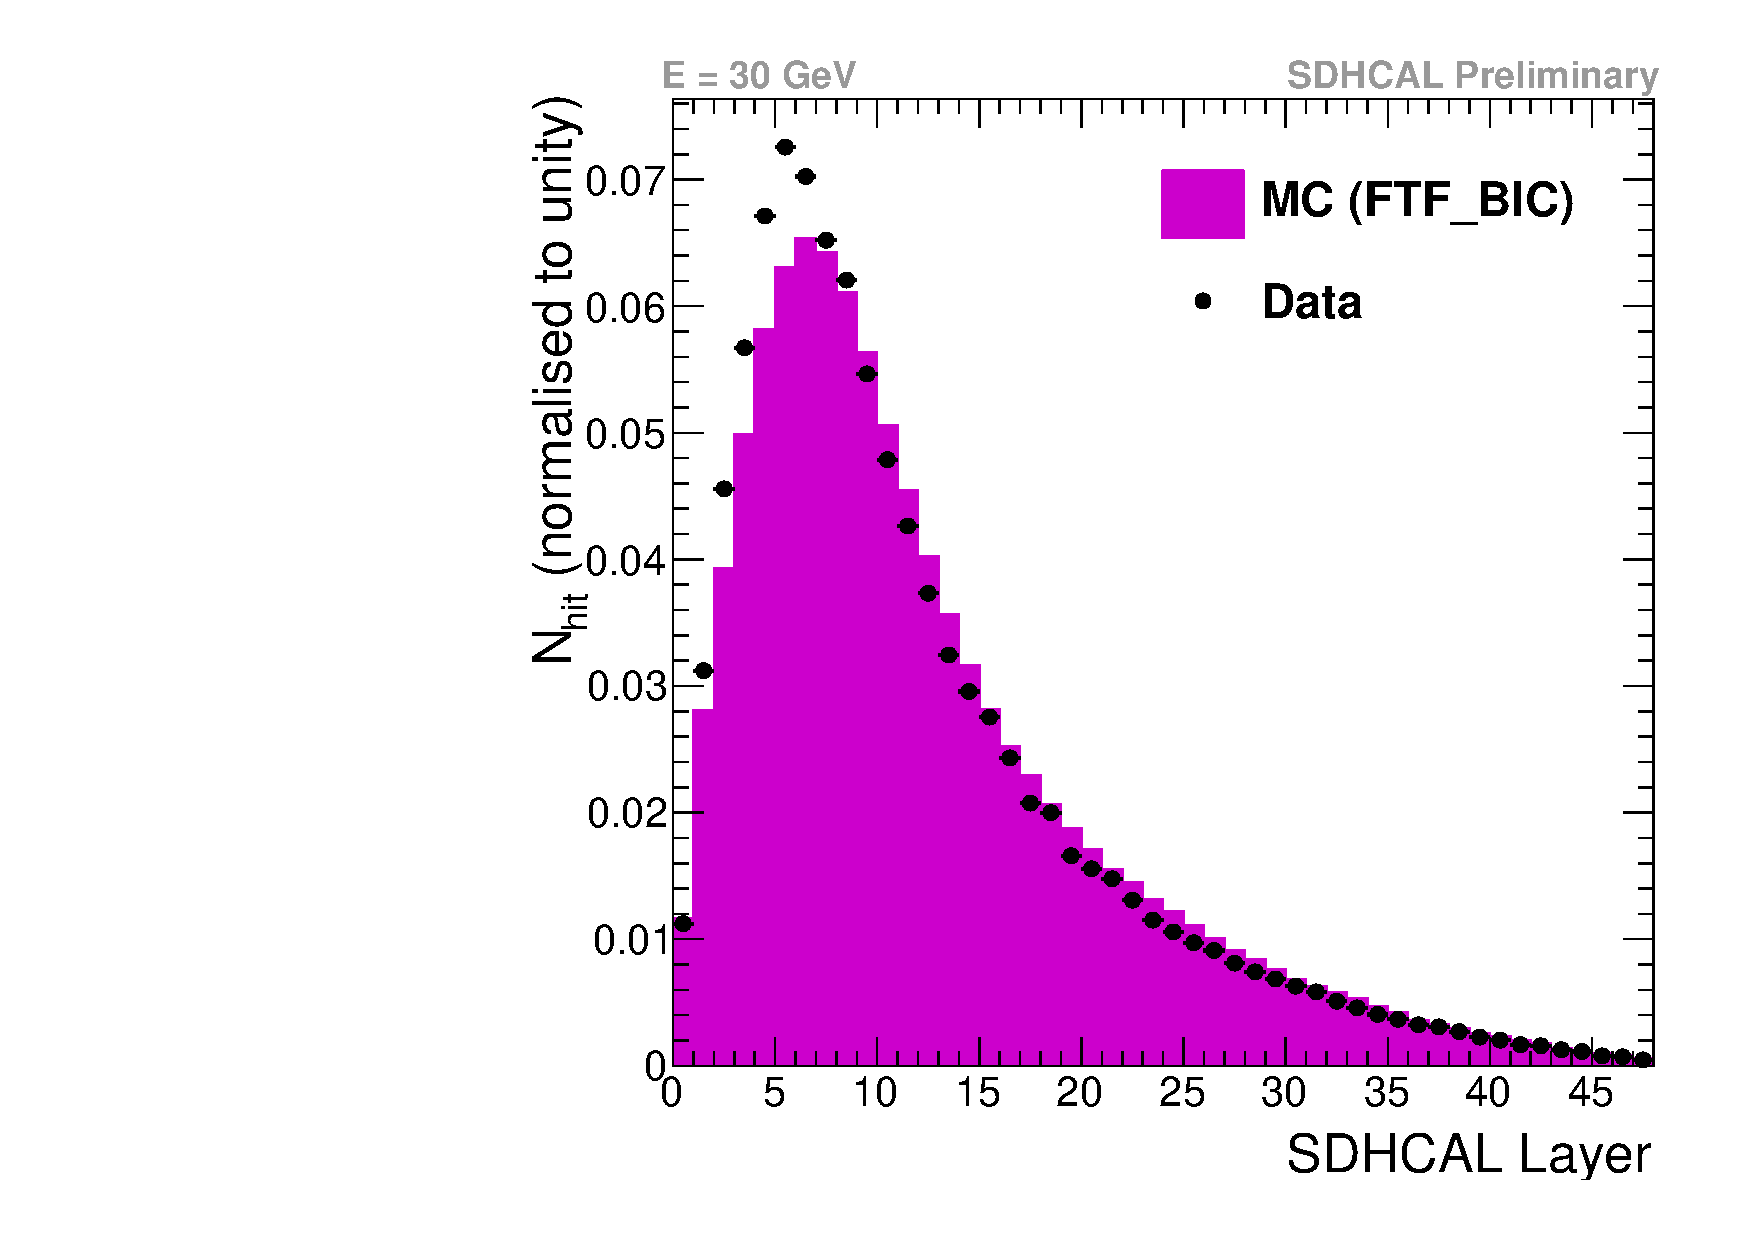
\includegraphics[width=.32\textwidth]{Shower/figs/longiProf_pi-_30GeV_ftf_bic.pdf}\\
  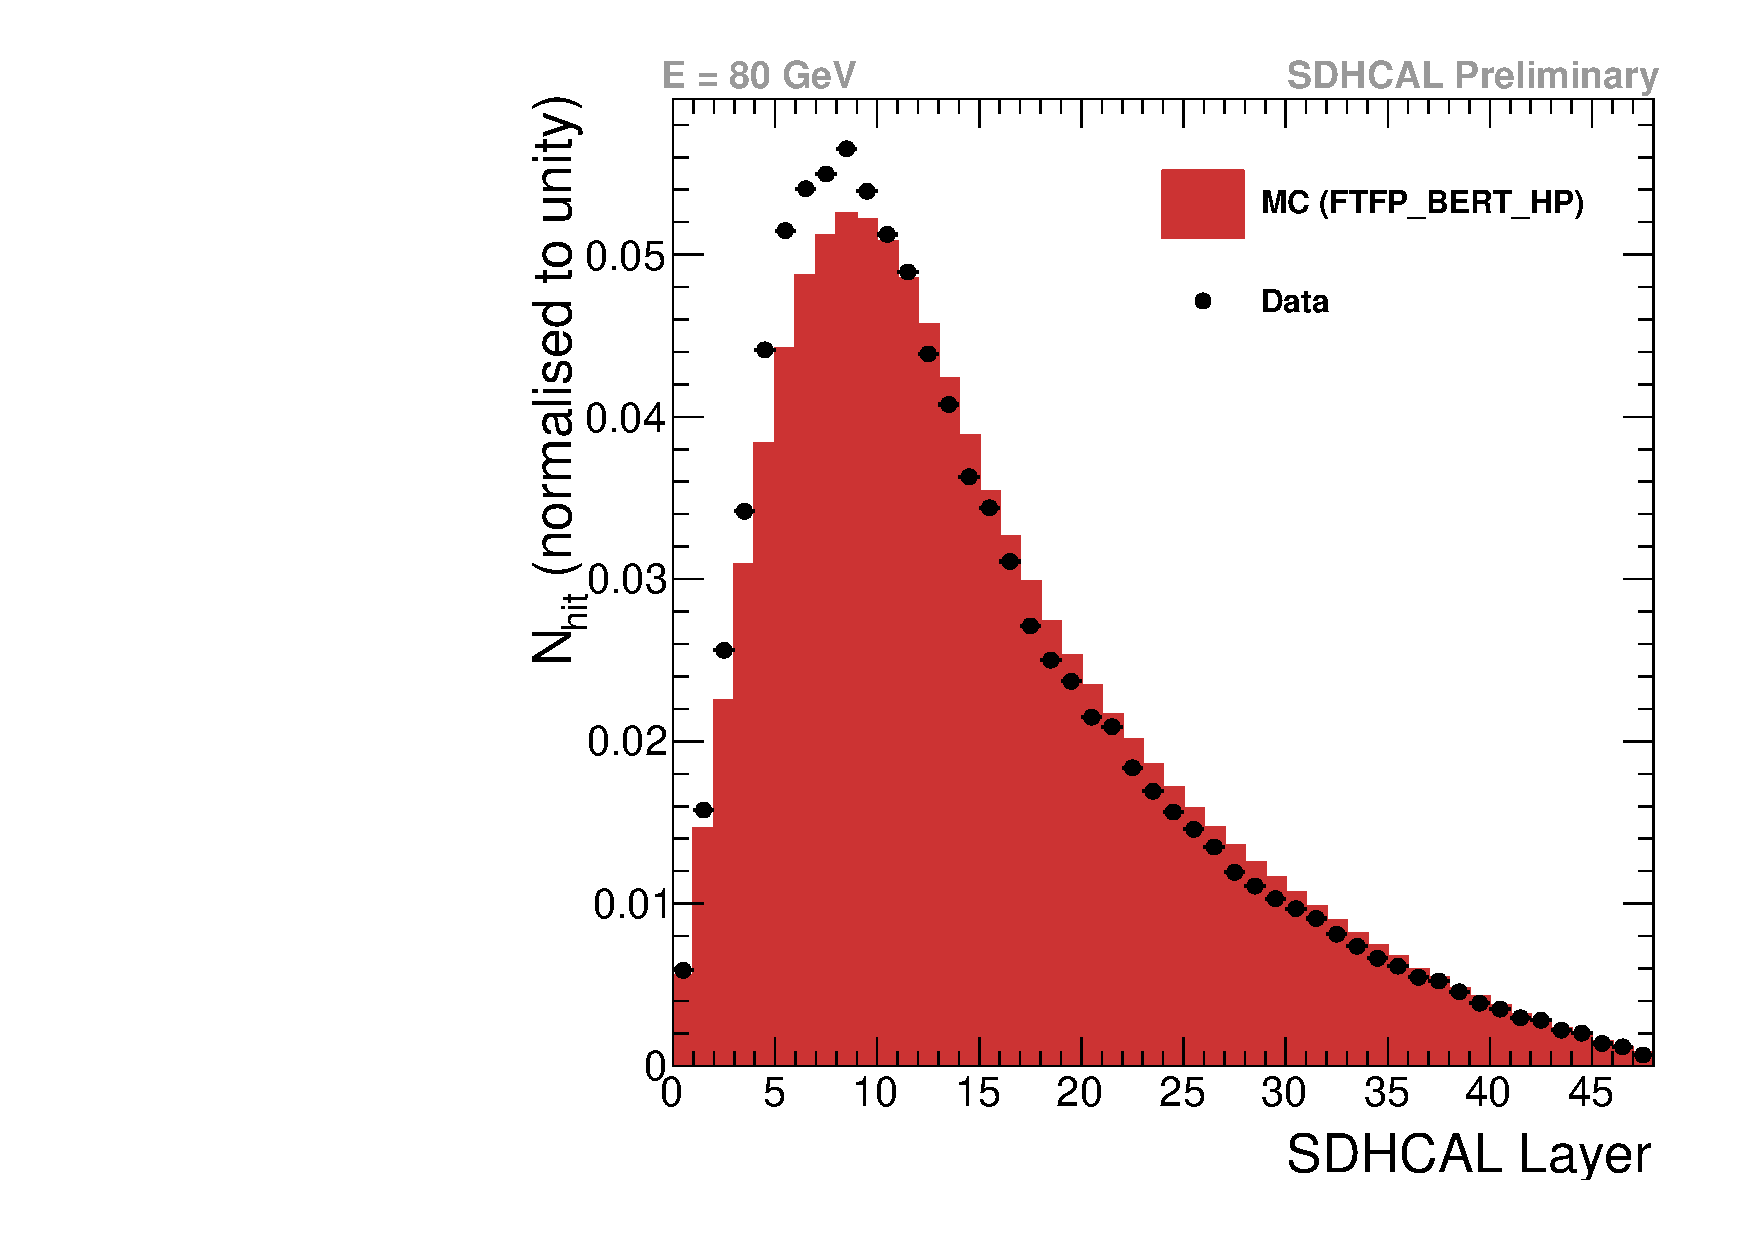
\includegraphics[width=.32\textwidth]{Shower/figs/longiProf_pi-_80GeV_ftfp_bert_hp.pdf}
  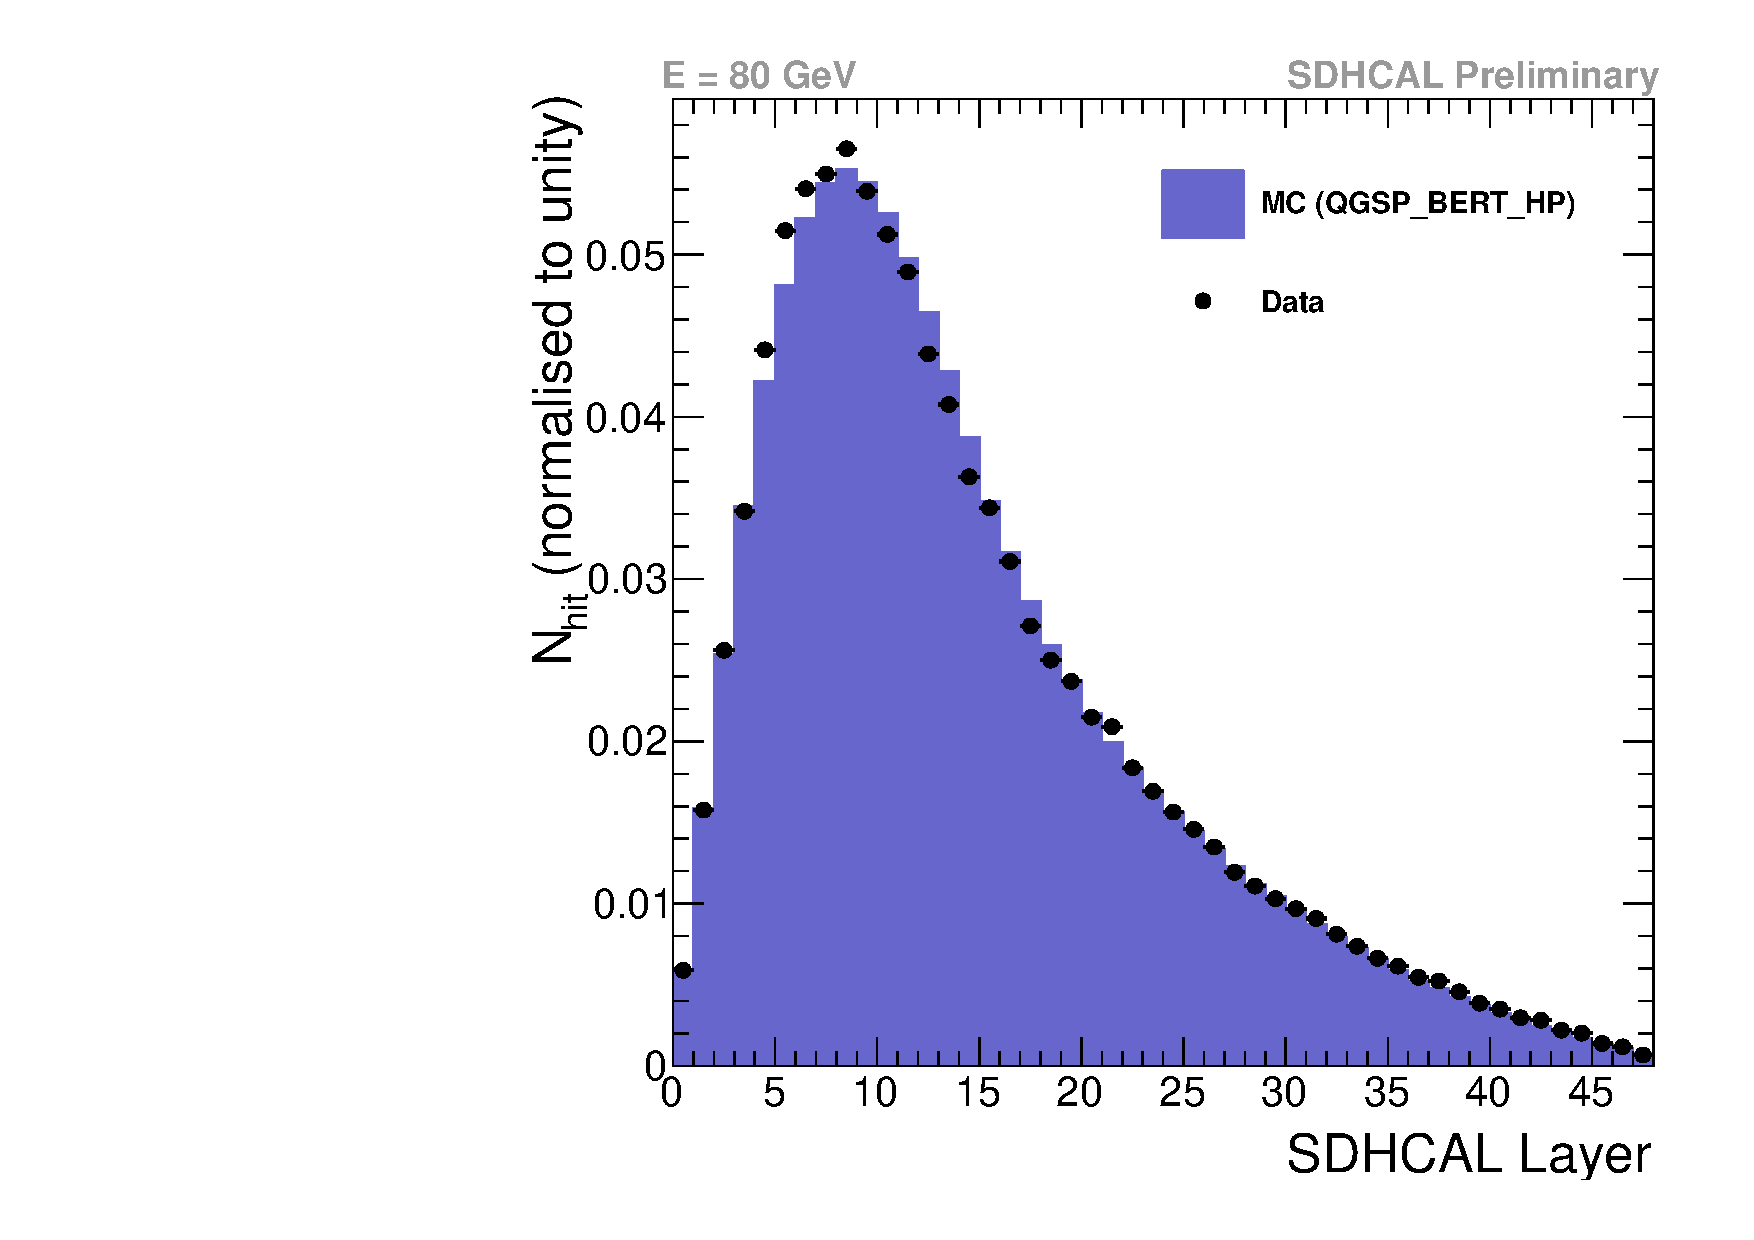
\includegraphics[width=.32\textwidth]{Shower/figs/longiProf_pi-_80GeV_qgsp_bert_hp.pdf}
  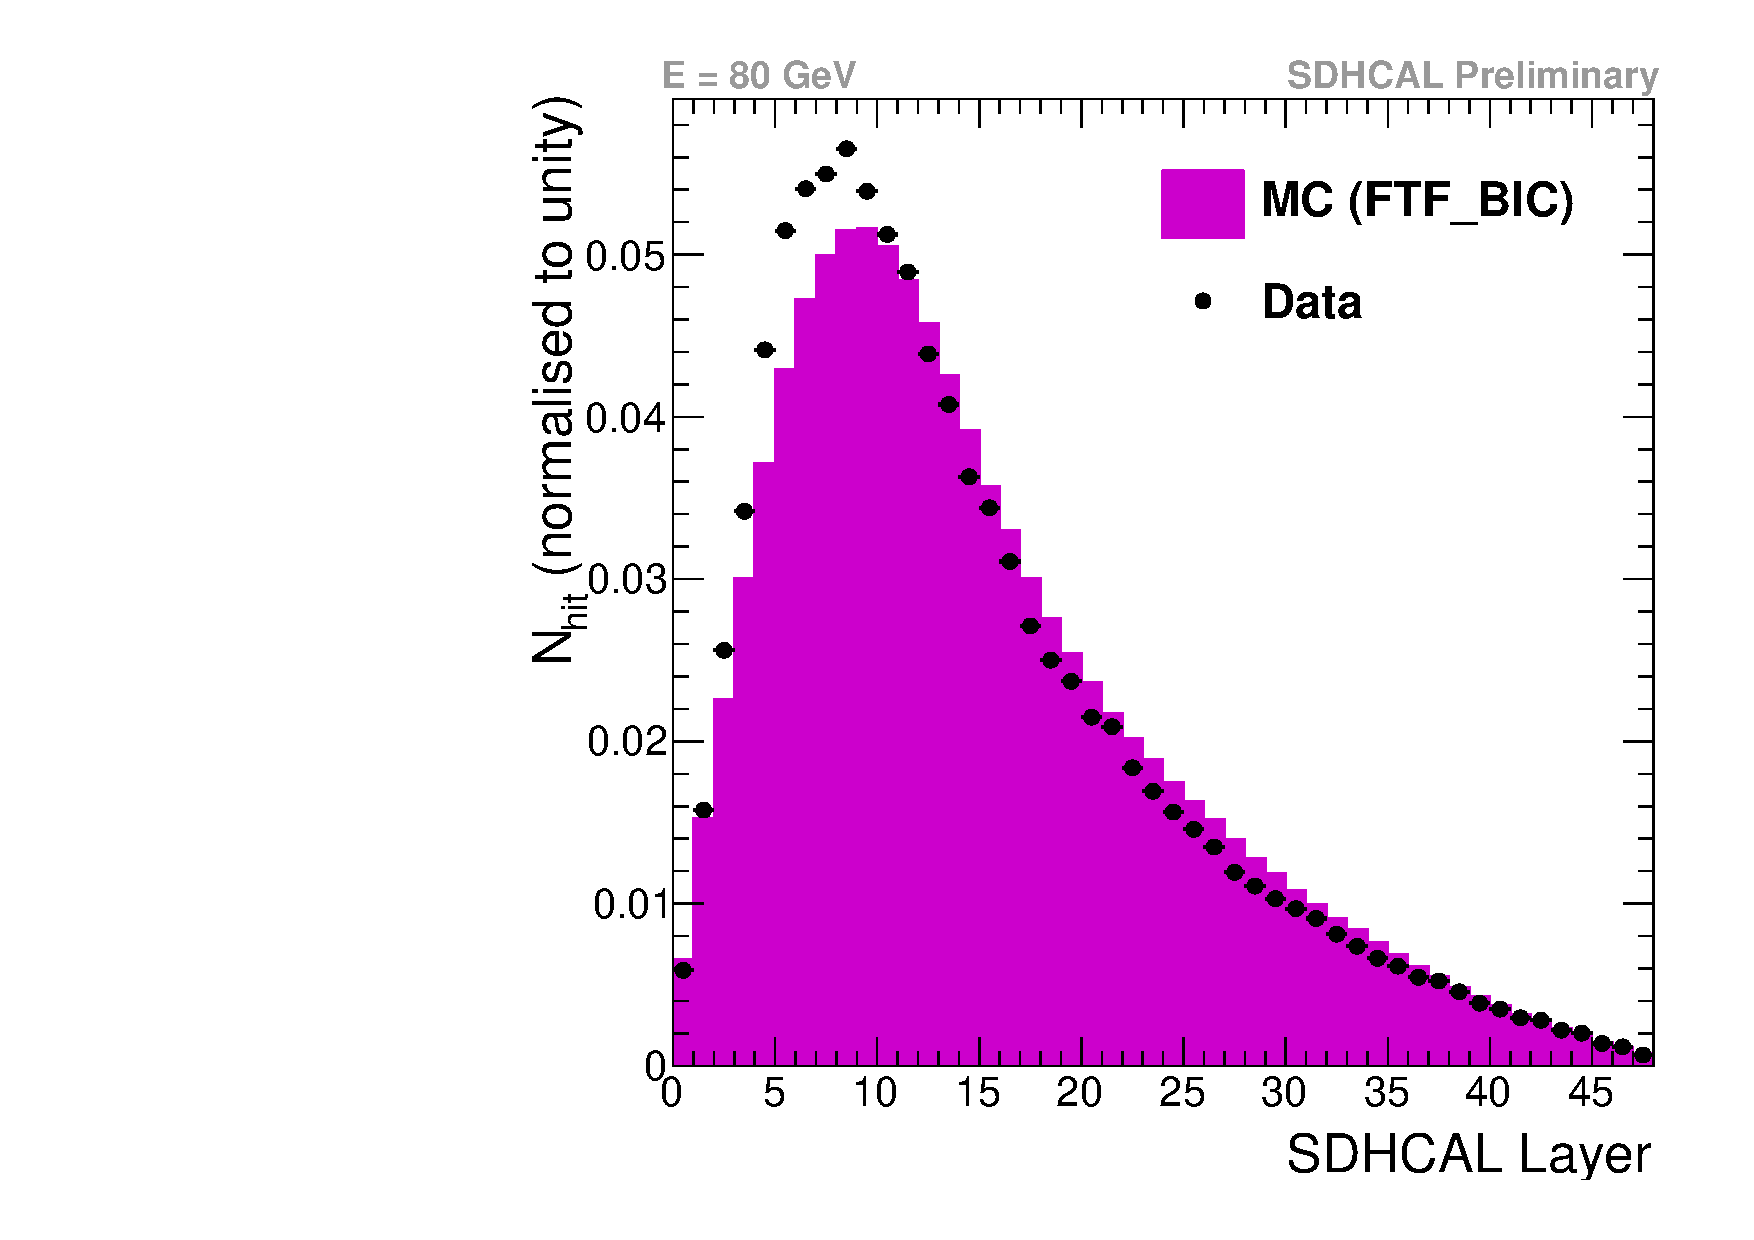
\includegraphics[width=.32\textwidth]{Shower/figs/longiProf_pi-_80GeV_ftf_bic.pdf}
  \caption{Profil longitudinal pour des échantillons de pions de 10 GeV (en haut), de 30 GeV (au milieu) et de 80 GeV (en bas) pour les données et des simulations réalisées avec les listes FTFP\_BERT\_HP (à gauche), QGSP\_BERT\_HP (au centre) et FTF\_BIC (à droite). Les données sont représentées par des cercles noirs et la simulation par les histogrammes pleins. \label{fig.pi-longi}}
\end{figure}
Le profil longitudinal est construit en calculant la moyenne du nombre de hits dans chaque plan sur un grand nombre d'événements. Le profil longitudinal correspond donc à la moyenne du nombre de hits en fonction de la profondeur dans le calorimètre. Le profil longitudinal peut être déterminé en comptant les cellules touchées à partir du premier plan du calorimètre ou à partir du premier plan d'interaction inélastique, défini dans la section~\ref{sec.pi_selection} du chapitre~\ref{chap.sdhcal}. Nous utiliserons dans la suite, le profil longitudinal relatif au premier plan d'interaction. %Cette méthode permet d'absorber les fluctuations du premier plan d'interaction. 
Les données expérimentales sont corrigées avec le temps du cycle du faisceau avec des polynômes de degré 2. Enfin, au vu des différences entre le nombre de hits dans les données et la simulation, le nombre de hits de chaque plan est normalisé au nombre total de hits dans l'événement. 
La figure~\ref{fig.pi-longi} présente le profil longitudinal pour les données et plusieurs listes physiques à 10, 30 et 80 $GeV$. Les listes physiques utilisant le modèle de Fritiof montrent des profils longitudinaux légèrement plus étendus que les données. L'accord entre les données et la liste physique QGSP\_BERT\_HP semble excellent. La valeur moyenne $<Z>$ des profils longitudinaux est donnée par:
\begin{equation}
  <Z>=\frac{1}{N_{event}}\sum_{i=0}^{N_{event}}\sum_{k=0}^{k_{max}}k\frac{N_{k,i}}{N_{tot,i}}
\end{equation}
où $N_{event}$ est le nombre d'événements, $N_{k,i}$ est le nombre de hits dans le plan $k$ pour l'événement $i$ et $N_{tot,i}$ est le nombre total de hits pour l'événement $i$. Le numéro de chaque plan $k$ est compté relativement par rapport au premier plan d'interaction. $k_{max}$ correspond alors à la profondeur effectivement restante.
\begin{figure}[!ht]
  \centering
  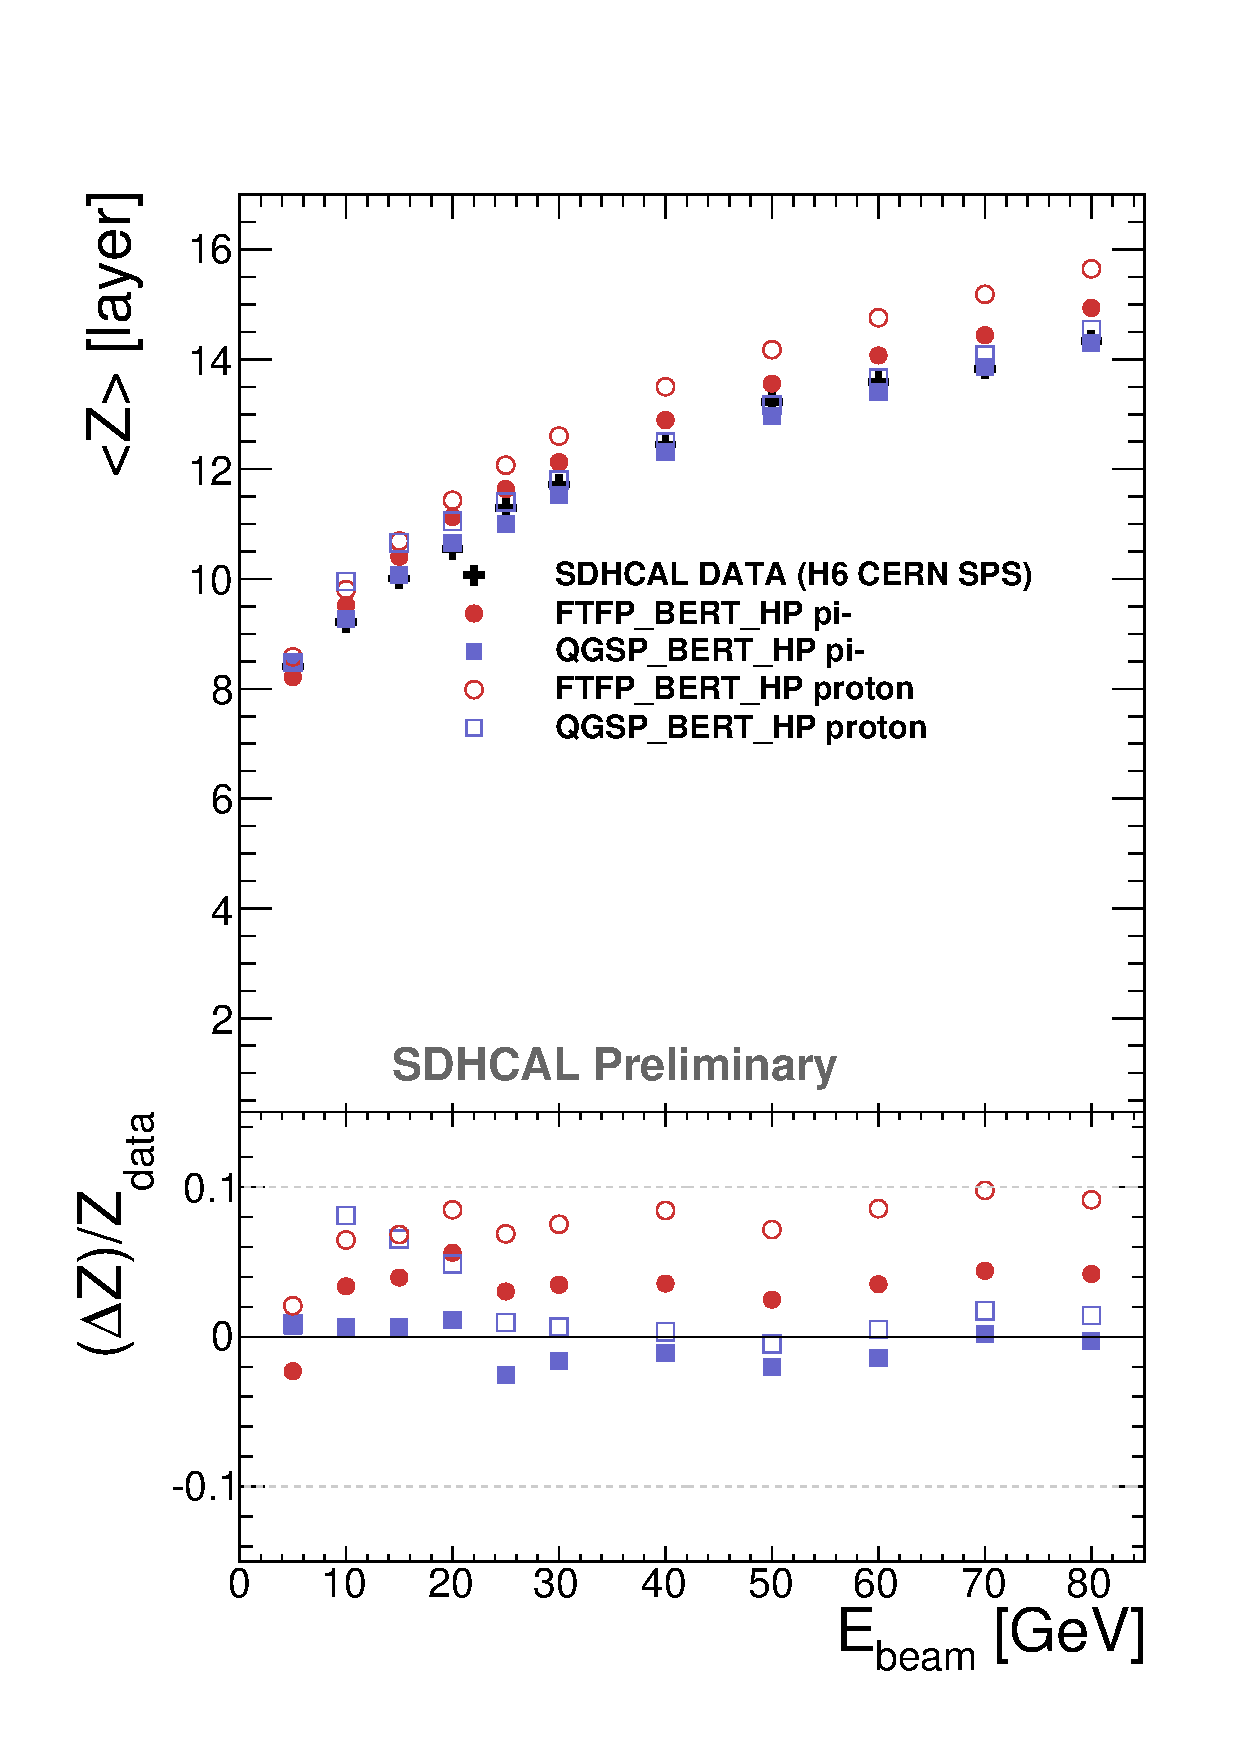
\includegraphics[width=.48\textwidth]{Shower/figs/LONGIPION.pdf}
  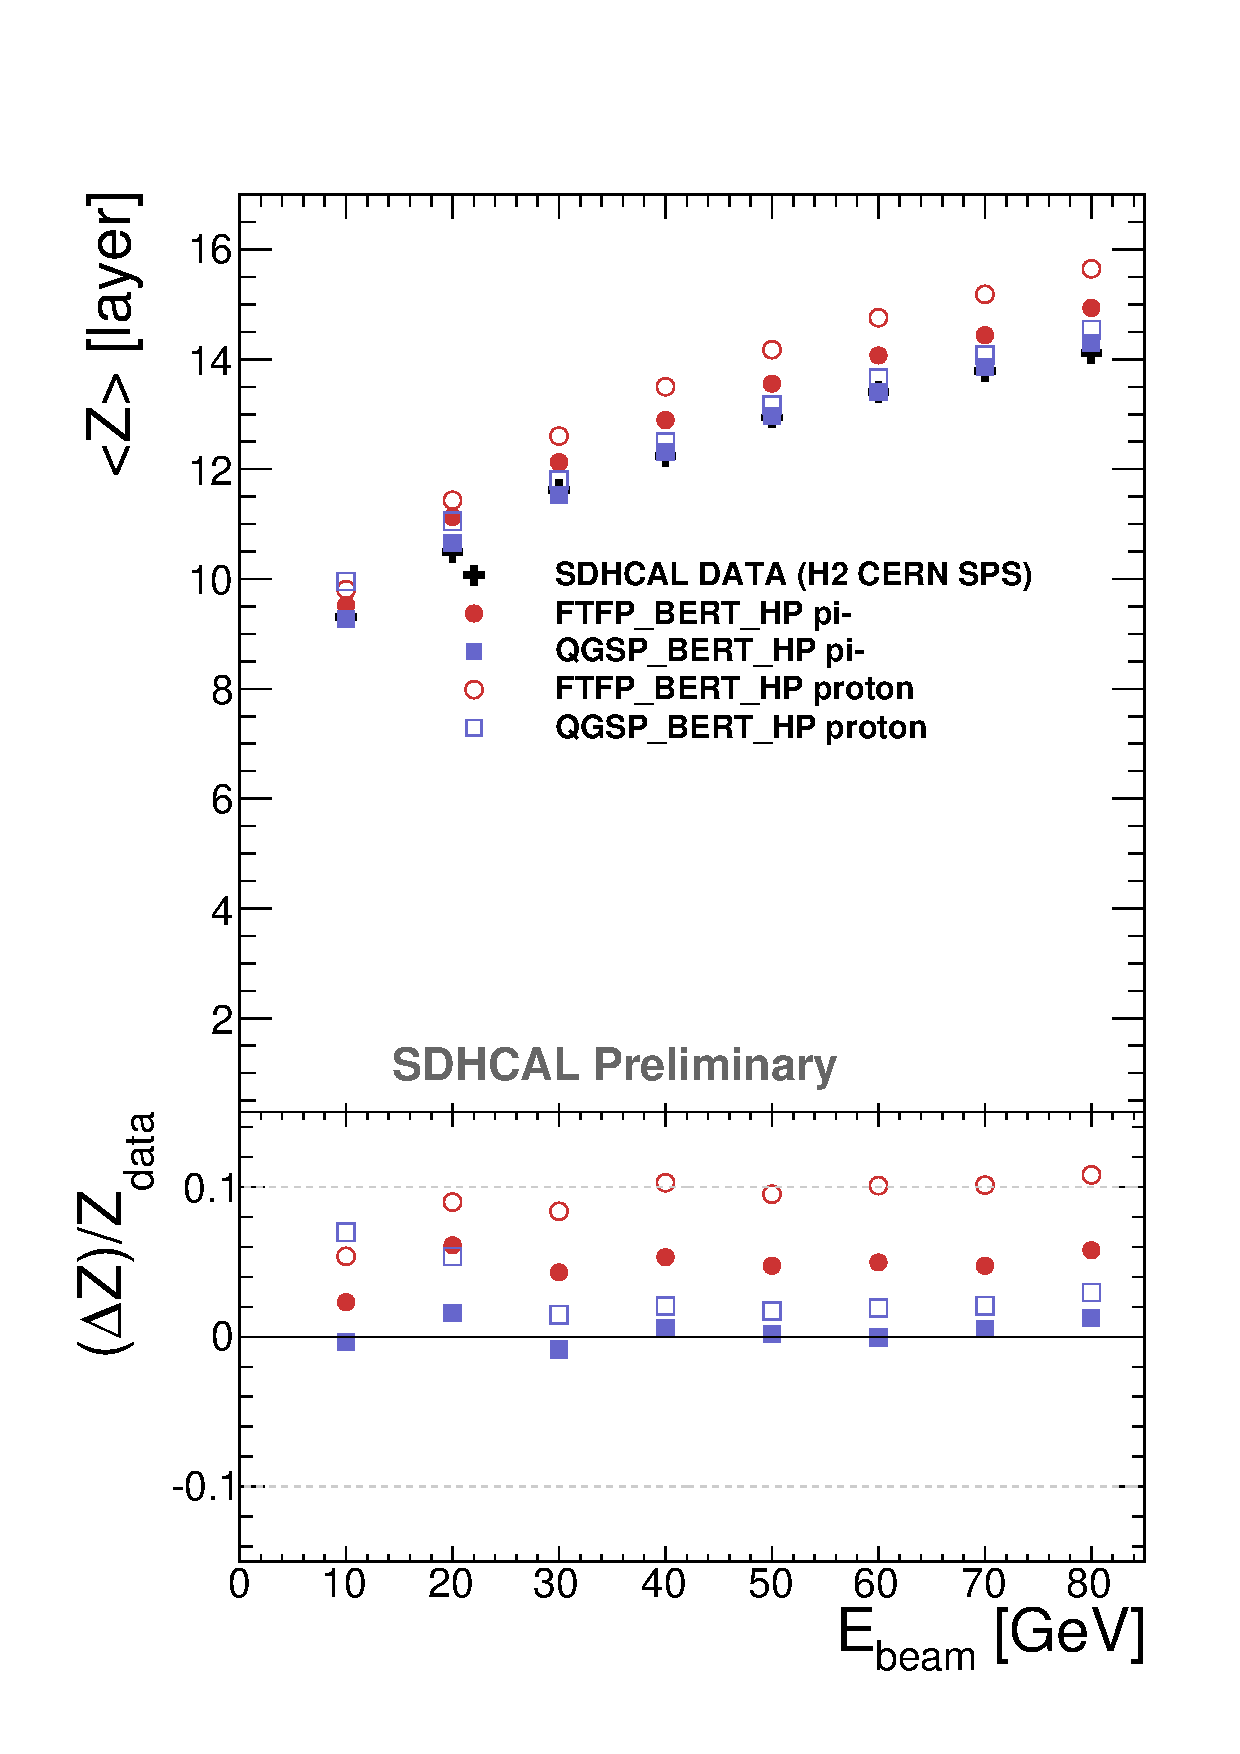
\includegraphics[width=.48\textwidth]{Shower/figs/LONGIPIONNOV.pdf}
  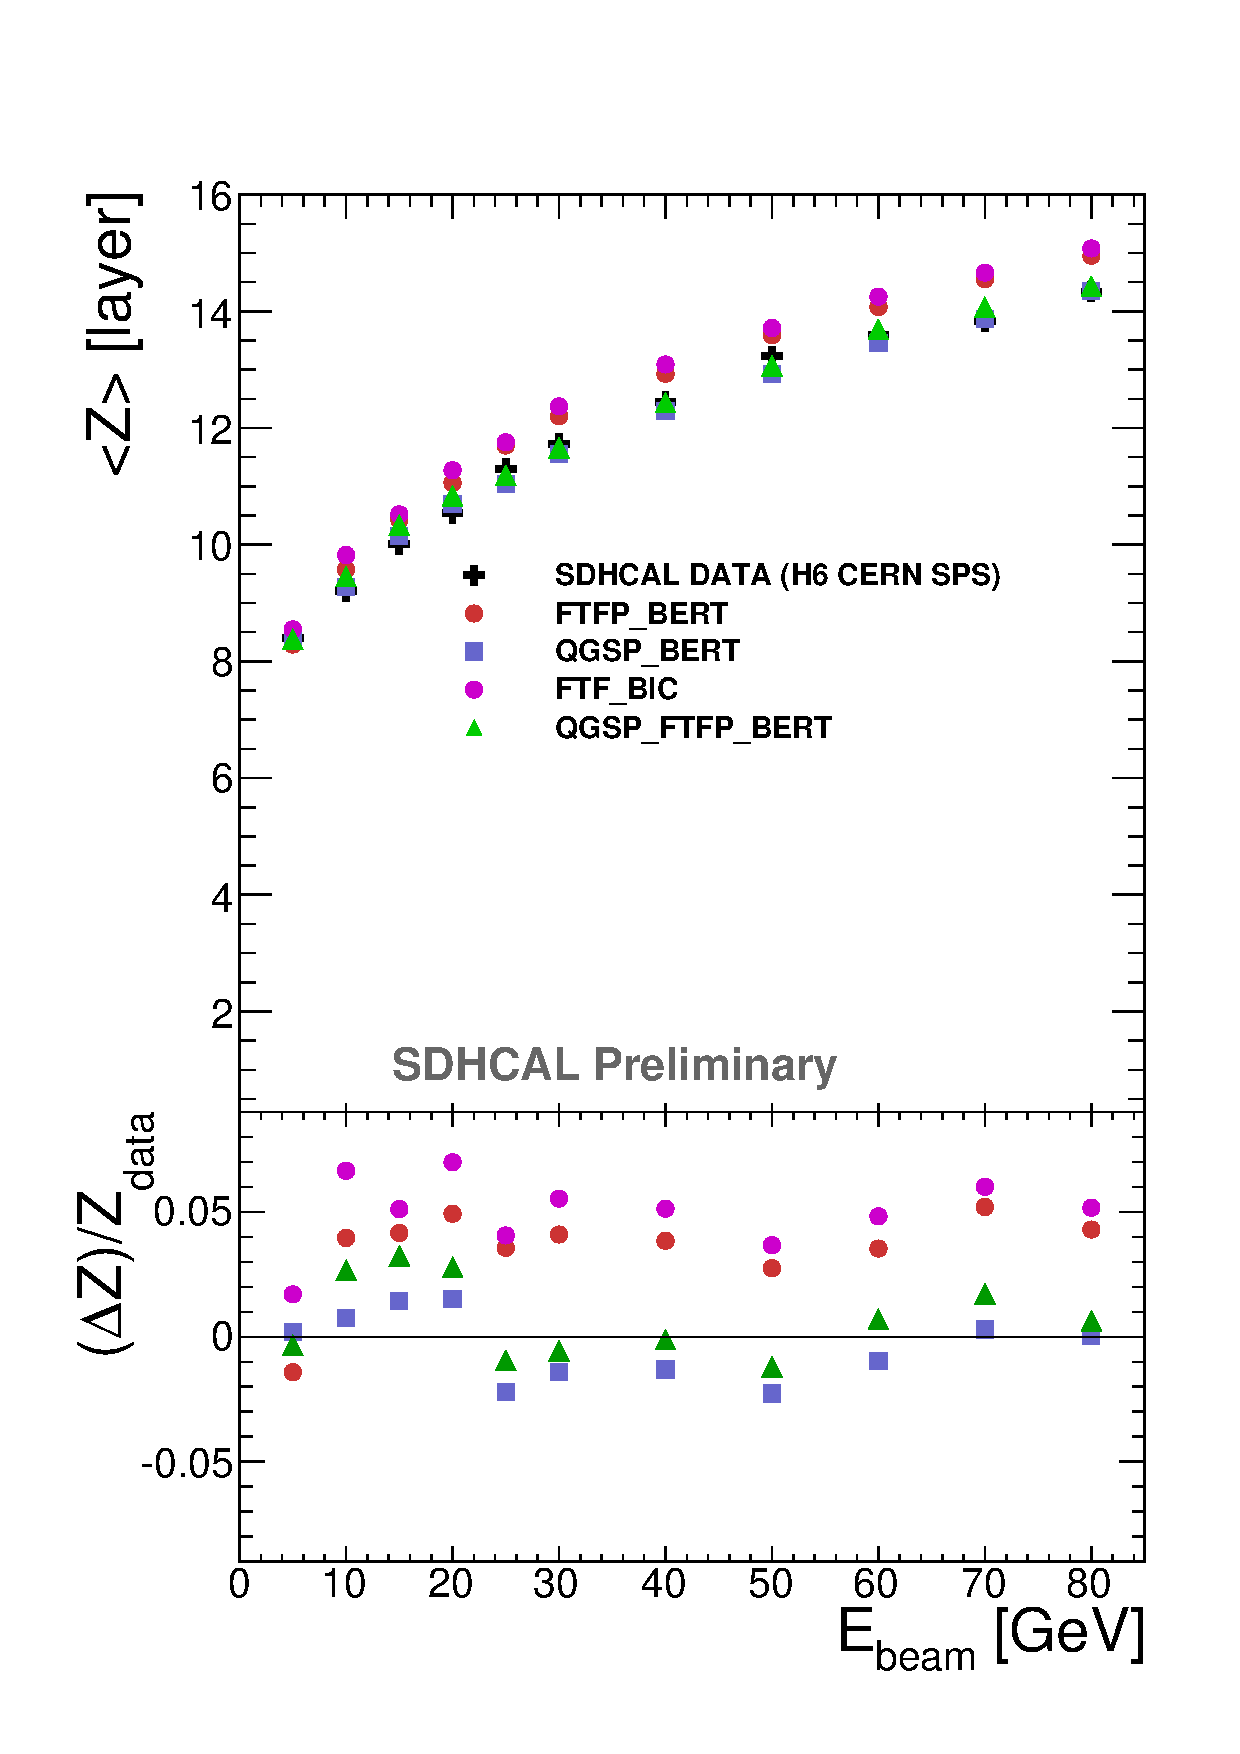
\includegraphics[width=.48\textwidth]{Shower/figs/LONGIPROF_PION_MODEL.pdf}
  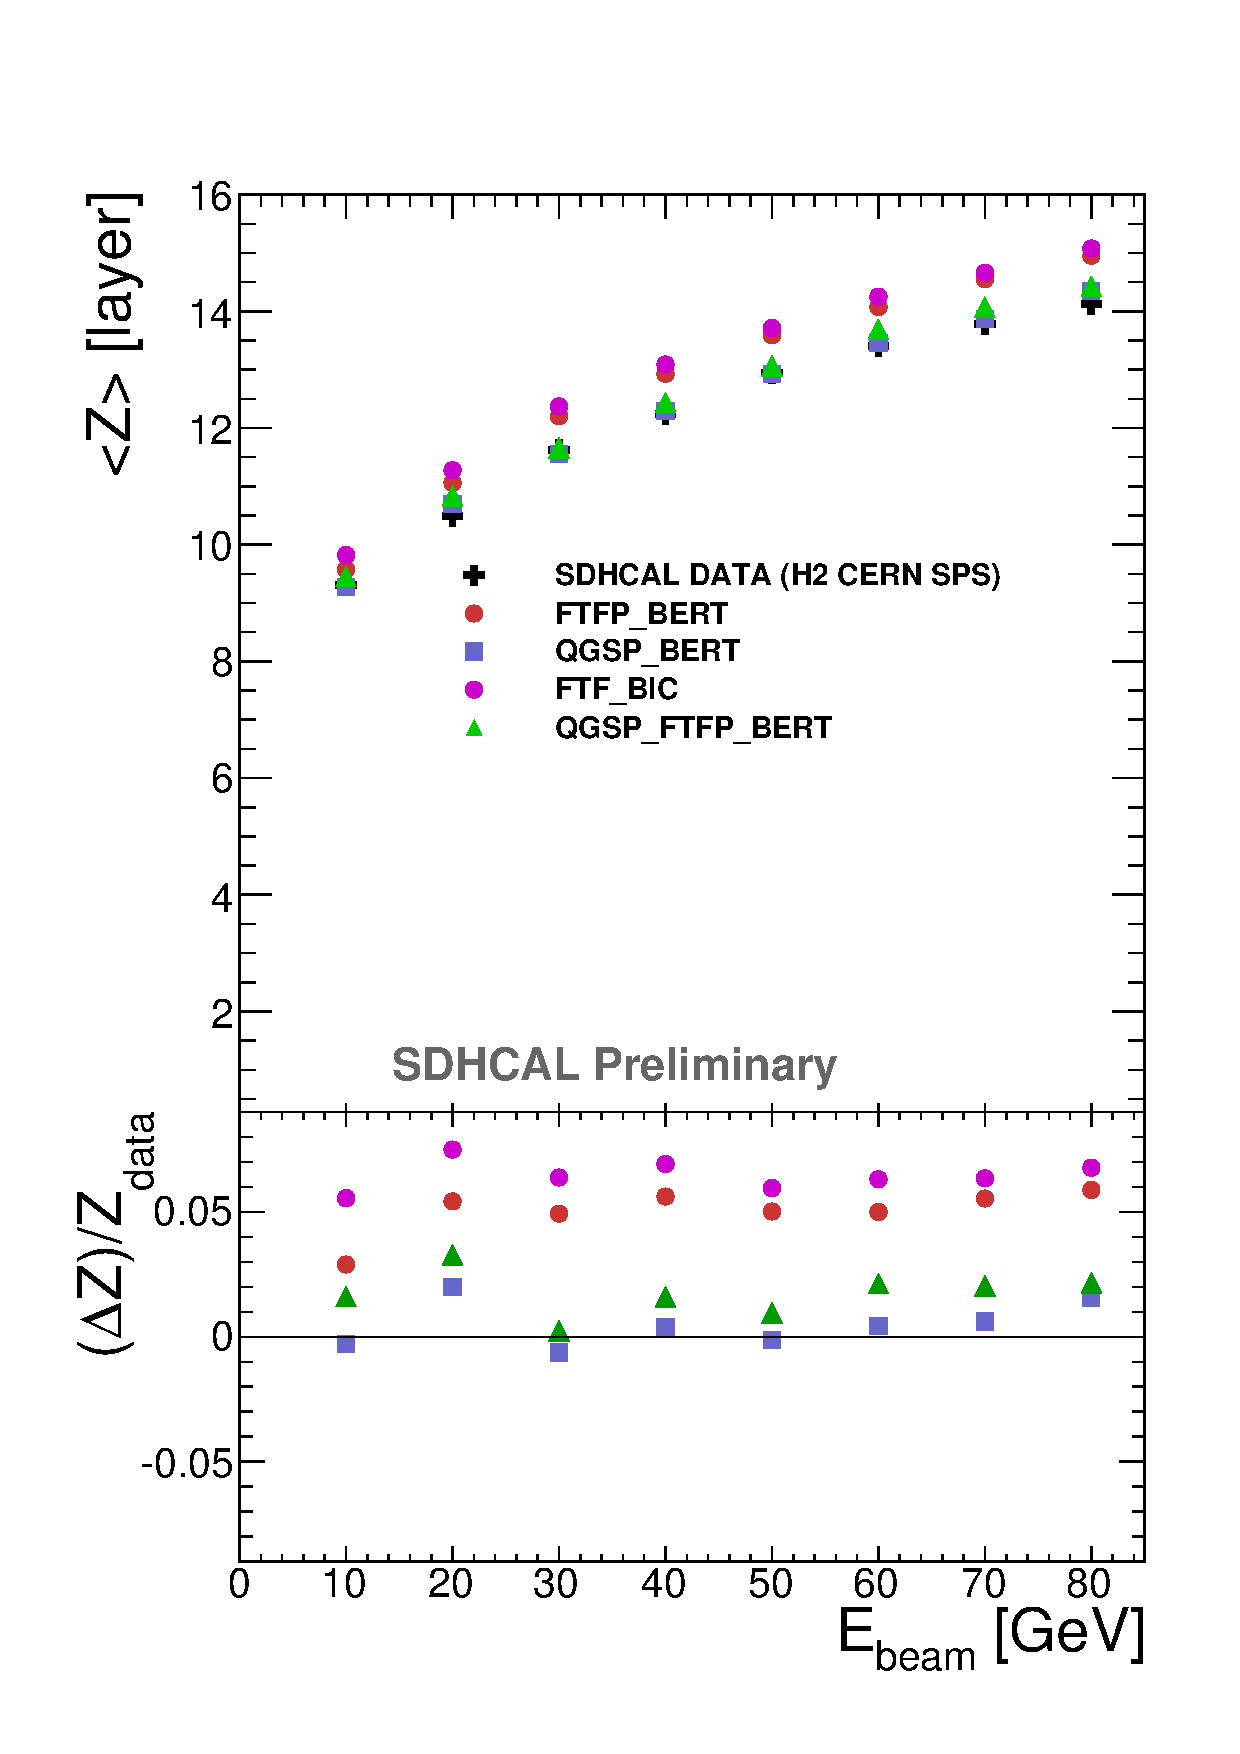
\includegraphics[width=.48\textwidth]{Shower/figs/LONGIPROF_PION_MODEL_NOV.pdf}
  \caption{Valeur moyenne et déviation relative du profil longitudinal en fonction de l'énergie du faisceau pour les données enregistrées sur les lignes H6 (à gauche) et H2 (à droite) et plusieurs listes physiques. Les figures du haut montrent aussi les résultats pour des simulations initiées par des protons. La taille des barres d'erreurs est inférieure à celle des points.}
  \label{fig.longi_pi-_ebeam}
\end{figure}
La figure~\ref{fig.longi_pi-_ebeam} montre la valeur moyenne du profil longitudinal en fonction de l'énergie du faisceau pour les données et plusieurs listes physiques et la déviation relative, définie par $\frac{<Z_{simu}>-<Z_{data}>}{<Z_{data}>}$. 

Les tendances aperçues sur les profils précédent se confirment. Les listes physiques utilisant le modèle de Fritiof pour les interactions de haute énergie ($E > 10~GeV$) surestiment légèrement l'extension longitudinale des gerbes hadroniques. Dans la section~\ref{sec.resultats} du chapitre~\ref{chap.simulation}, nous avions mentionné que la correction du problème dans le modèle de Fritiof, à partir de la version 10.1 de GEANT4, tend à diminuer l'extension des gerbes hadroniques. Les premiers tests effectués avec cette version de GEANT4 ne permettent pas d'obtenir des améliorations sensibles. Les listes physiques QGSP\_BERT(\_HP) et QGSP\_FTFP\_BERT\footnote{Le modèle de Fritiof est utilisé dans la liste QGSP\_FTFP\_BERT pour des énergies intermédiaire allant de 6 à 25 $GeV$ mais est exclusivement utilisé de 8 à 12 $GeV$.} présentent un bon accord avec les données. Enfin, notons que les gerbes hadroniques initiées par des protons présentent un profil longitudinal plus étendu que celles initiées par les pions. Ces différences, qui sont plus marquées pour la liste FTFP\_BERT\_HP que pour QGSP\_BERT\_HP, peuvent encore s'expliquer par la différence de la fraction élémagnétique entre les cascades initiées par des protons et par des pions. 

Le profil longitudinal des gerbes électromagnétiques de 20 $GeV$ est donné sur la figure~\ref{fig.longi_e-}(a) pour les données et une simulation. 
\begin{figure}[!ht]
  \subfigure[]{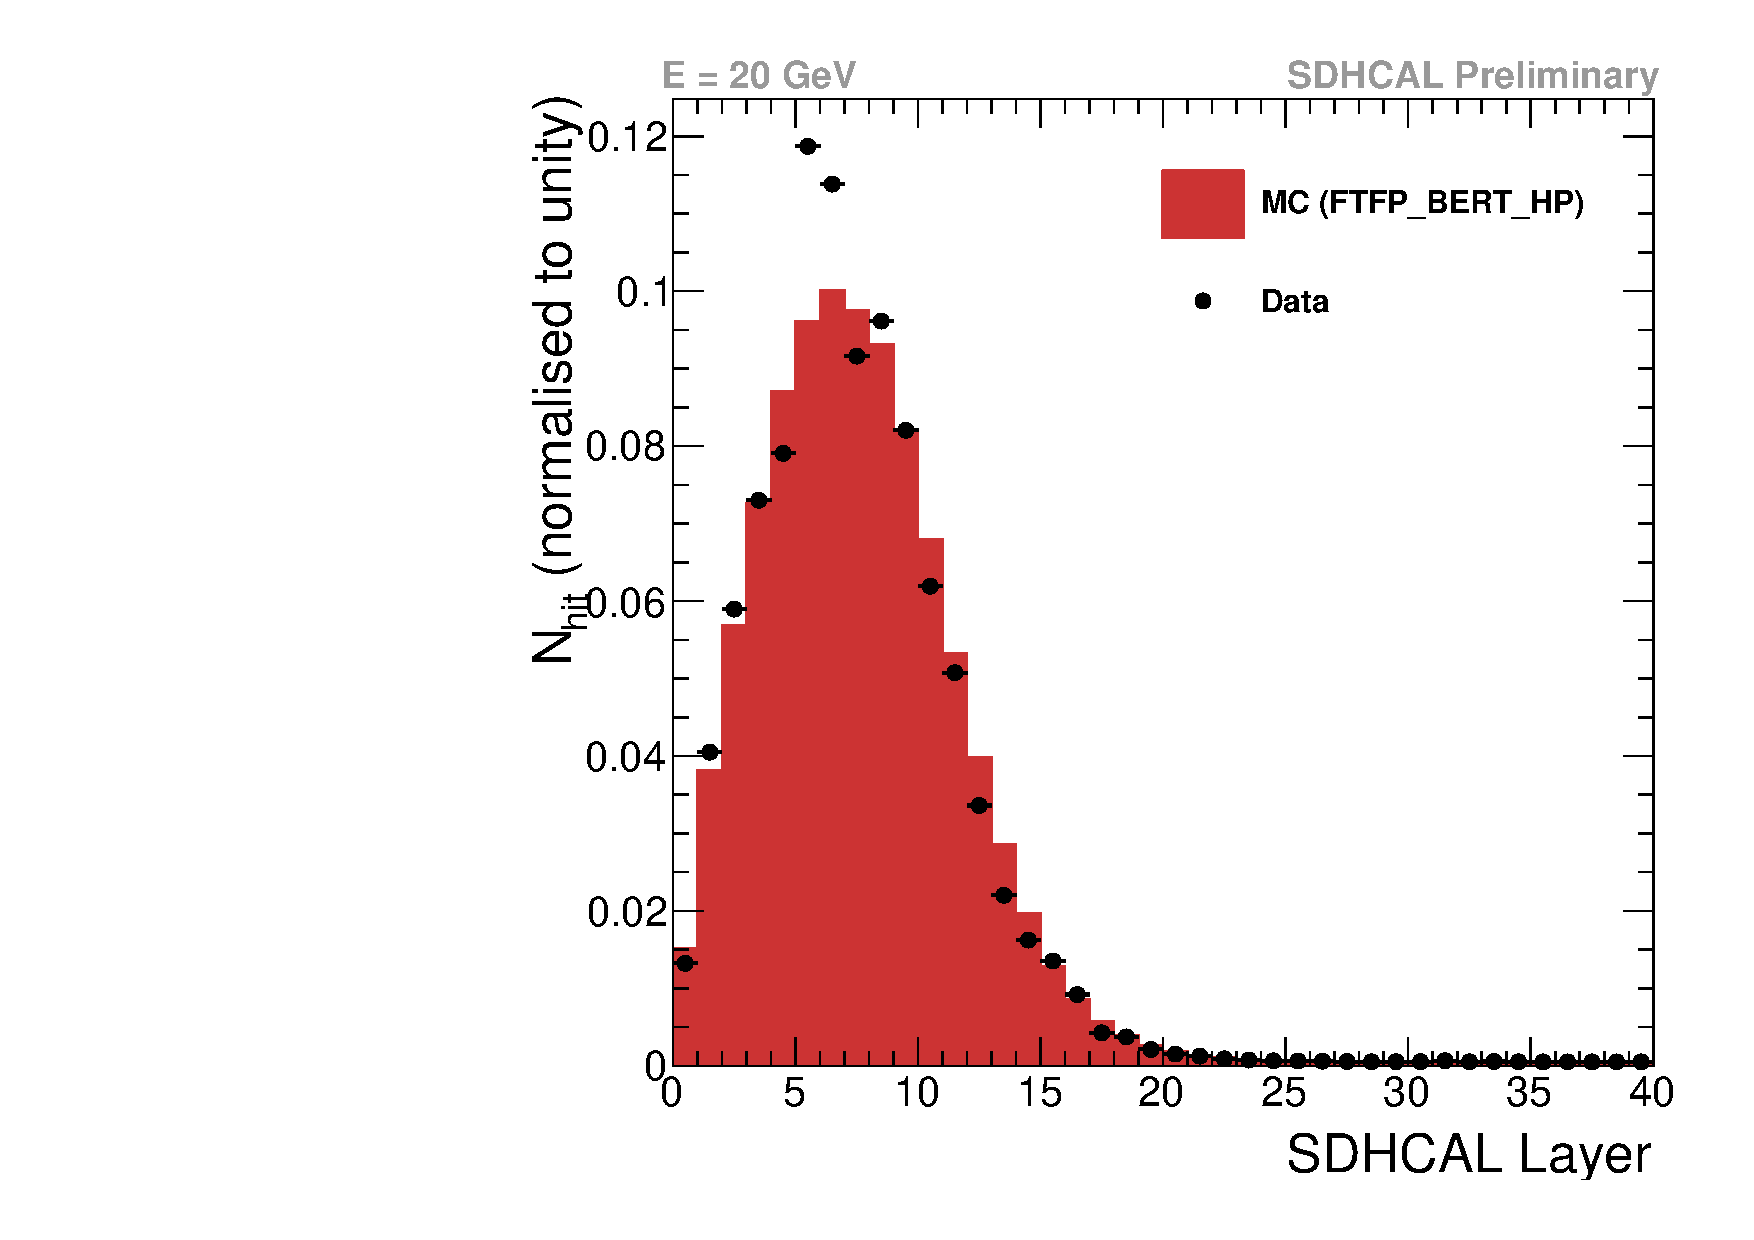
\includegraphics[width=.5\textwidth]{Shower/figs/longiProf_e-_20GeV_AugSep2012.pdf}}
  \subfigure[]{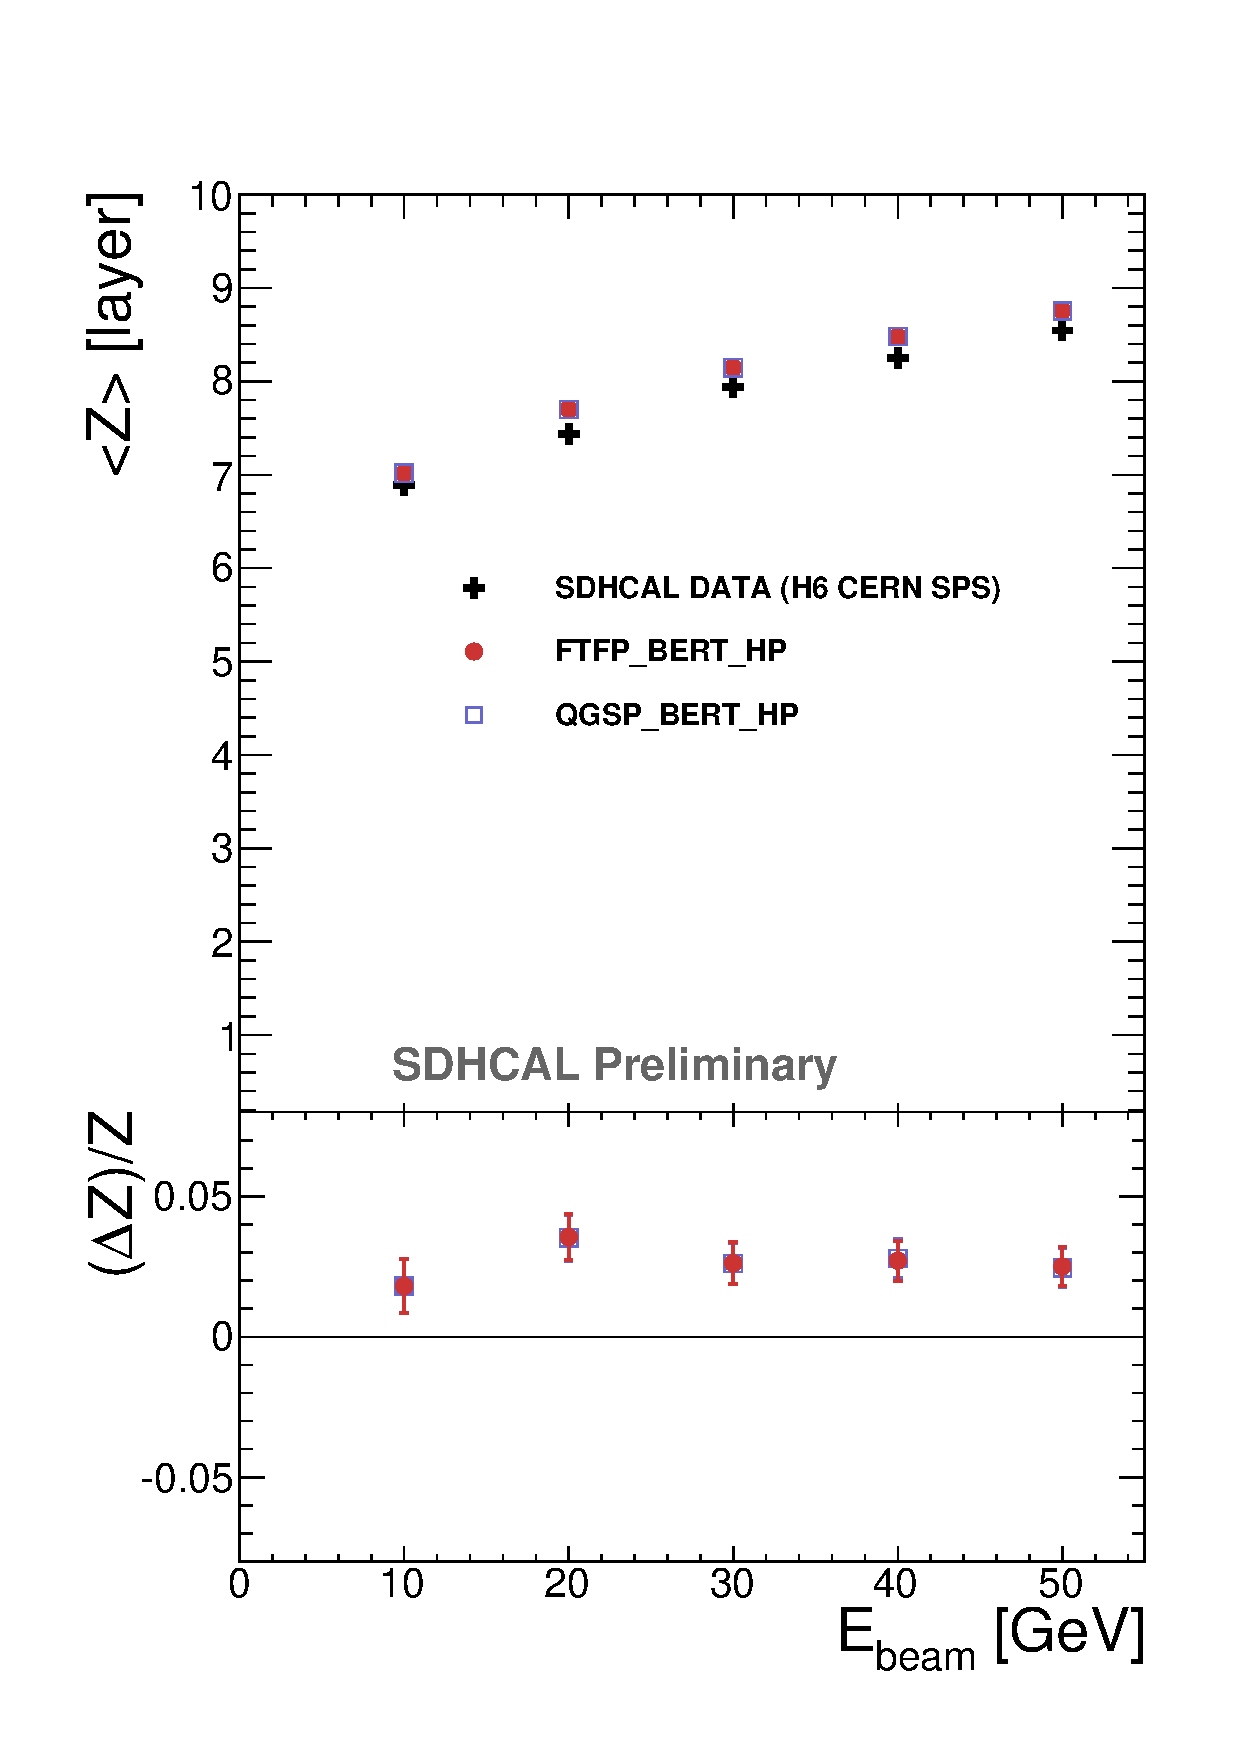
\includegraphics[width=.4\textwidth]{Shower/figs/LONGIELECTRON.pdf}}
  \caption{(a): Profil longitudinal de gerbes électromagnétiques à 20 $GeV$ pour les données (cercles noirs) et une simulation réalisée avec liste physique FTFP\_BERT\_HP (histogramme rouge). (b) Valeur moyenne et déviation relative du profil longitudinal pour des gerbes électromagnétiques en fonction de l'énergie du faisceau.}
  \label{fig.longi_e-}
\end{figure}
Des différences importantes, entre les données et la simulation, sont observées sur certains plans. Ces différences s'expliquent, comme pour la multiplicité, par des variations de résistivité de la peinture sur les plaques de verre. Cet effet n'est pas observé dans le cas des gerbes hadroniques car leur premier plan d'interaction varie, ce qui a pour conséquence de lisser le profil longitudinal. La longueur de radiation vaut 1.76 $cm$ dans l'acier, ce qui correspond à l'épaisseur de la première couche d'absorbeur (1.75 $cm$) avant la première GRPC du prototype. Le premier plan d'interaction d'une gerbe électromagnétique correspond donc très souvent au premier plan du détecteur. Malgré ces différences, l'accord entre données et simulations reste raisonnable et est confirmé par la figure~\ref{fig.longi_e-}(b), montrant la valeur moyenne du profil longitudinal des gerbes électromagnétiques en fonction de l'énergie. La déviation relative, aussi indiquée sur la figure~\ref{fig.longi_e-}(b), est inférieure à 4$\%$ sur toute la gamme d'énergie.

Nous avons vu que l'extension longitudinale des gerbes hadroniques est relativement bien simulée. Les listes physiques utilisant le modèle de Fritiof surestiment légèrement cette extension. Celles basées sur le modèle QGS, reproduisent bien l'extension longitudinale des gerbes hadroniques. Cette étude permet aussi de confirmer des études similaires qui ont été réalisées avec les calorimètres CALICE AHCAL \cite{geant4-ahcal} et CALICE Si-W ECAL \cite{naomi}. Ces études montrent que les listes physiques préparées par GEANT4 reproduisent convenablement l'extension longitudinale des gerbes hadroniques.

%%%%%%%%%%%%%%%%%%%%%%%%%%%%%%%%%%%%%%%%%%%%%%%
\newpage
\subsection{Profil latéral}
\label{sec.lateralProfil}
\begin{figure}[!ht]
  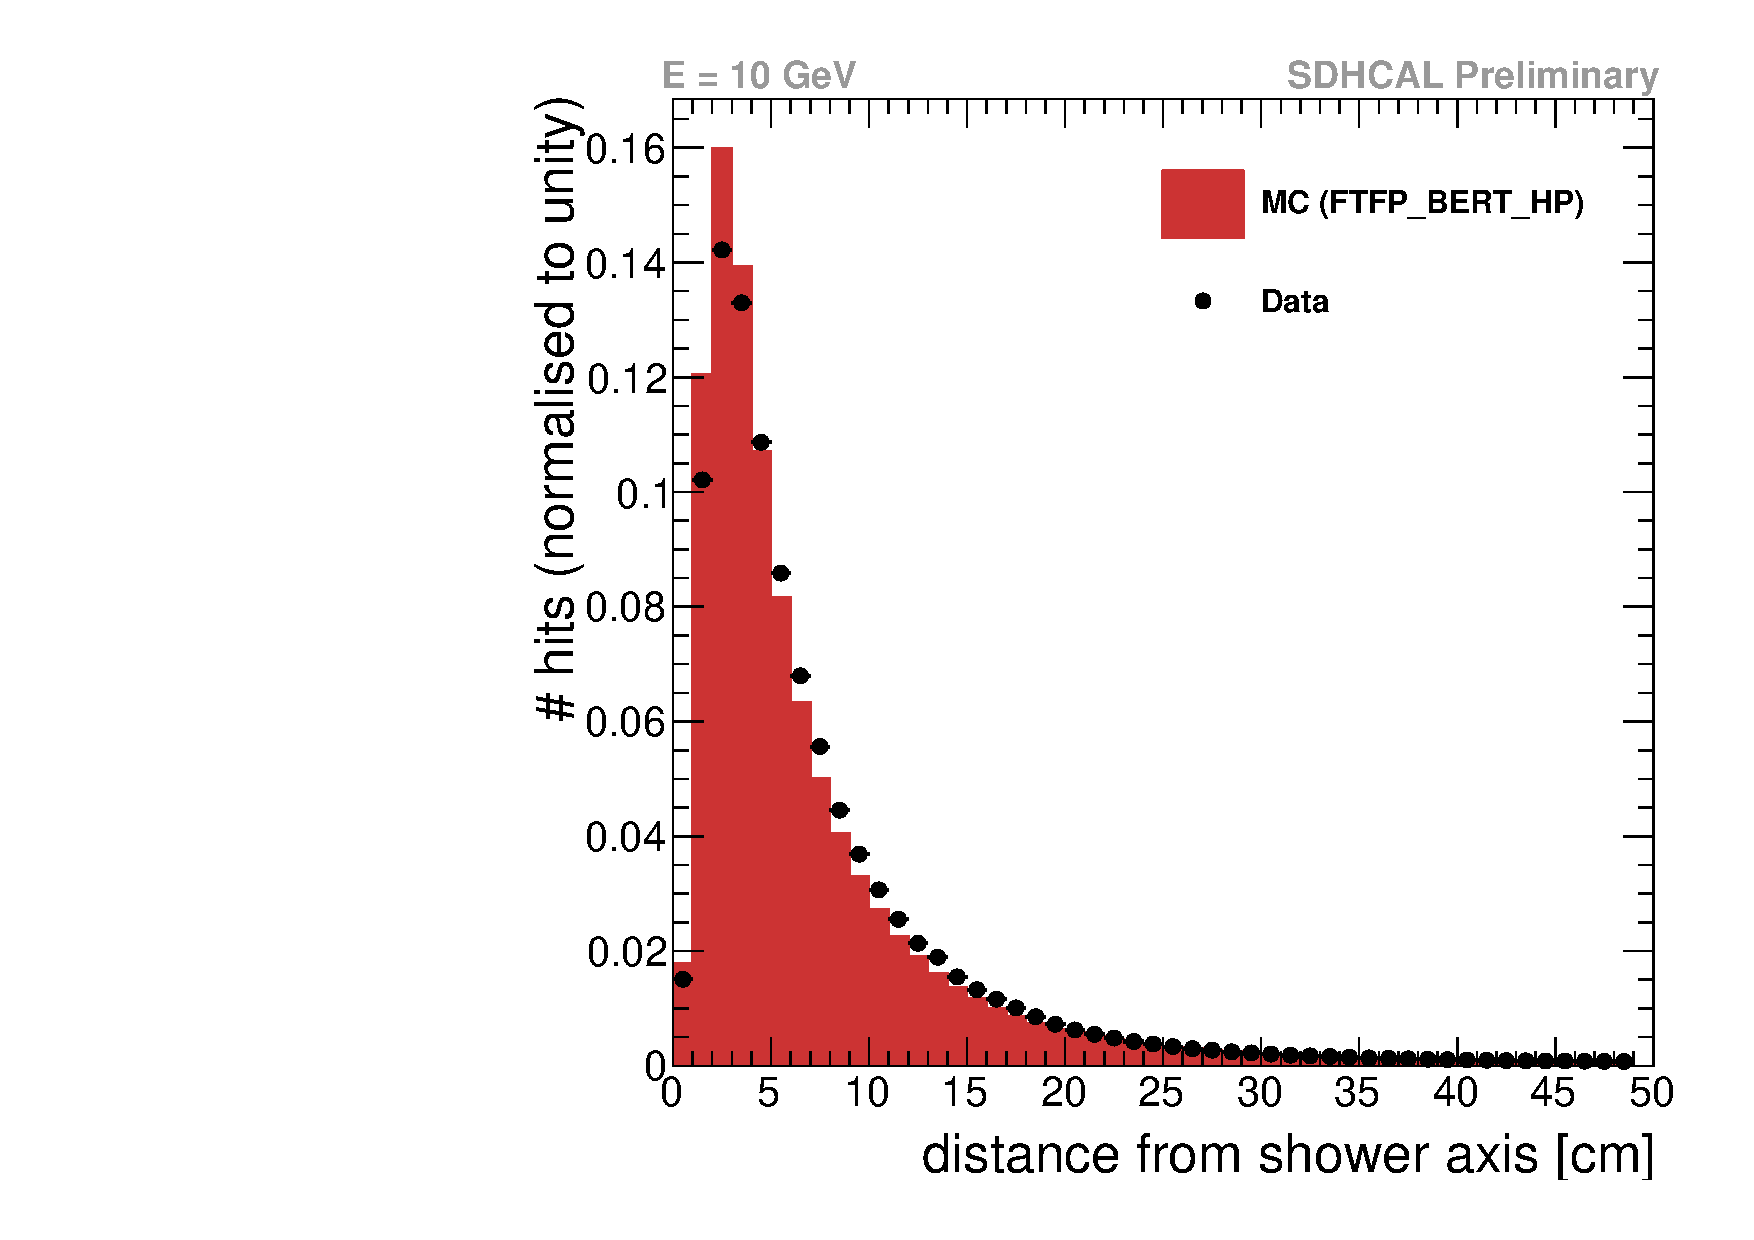
\includegraphics[width=.32\textwidth]{Shower/figs/radProf_pi-_10GeV_ftfp_bert_hp.pdf}
  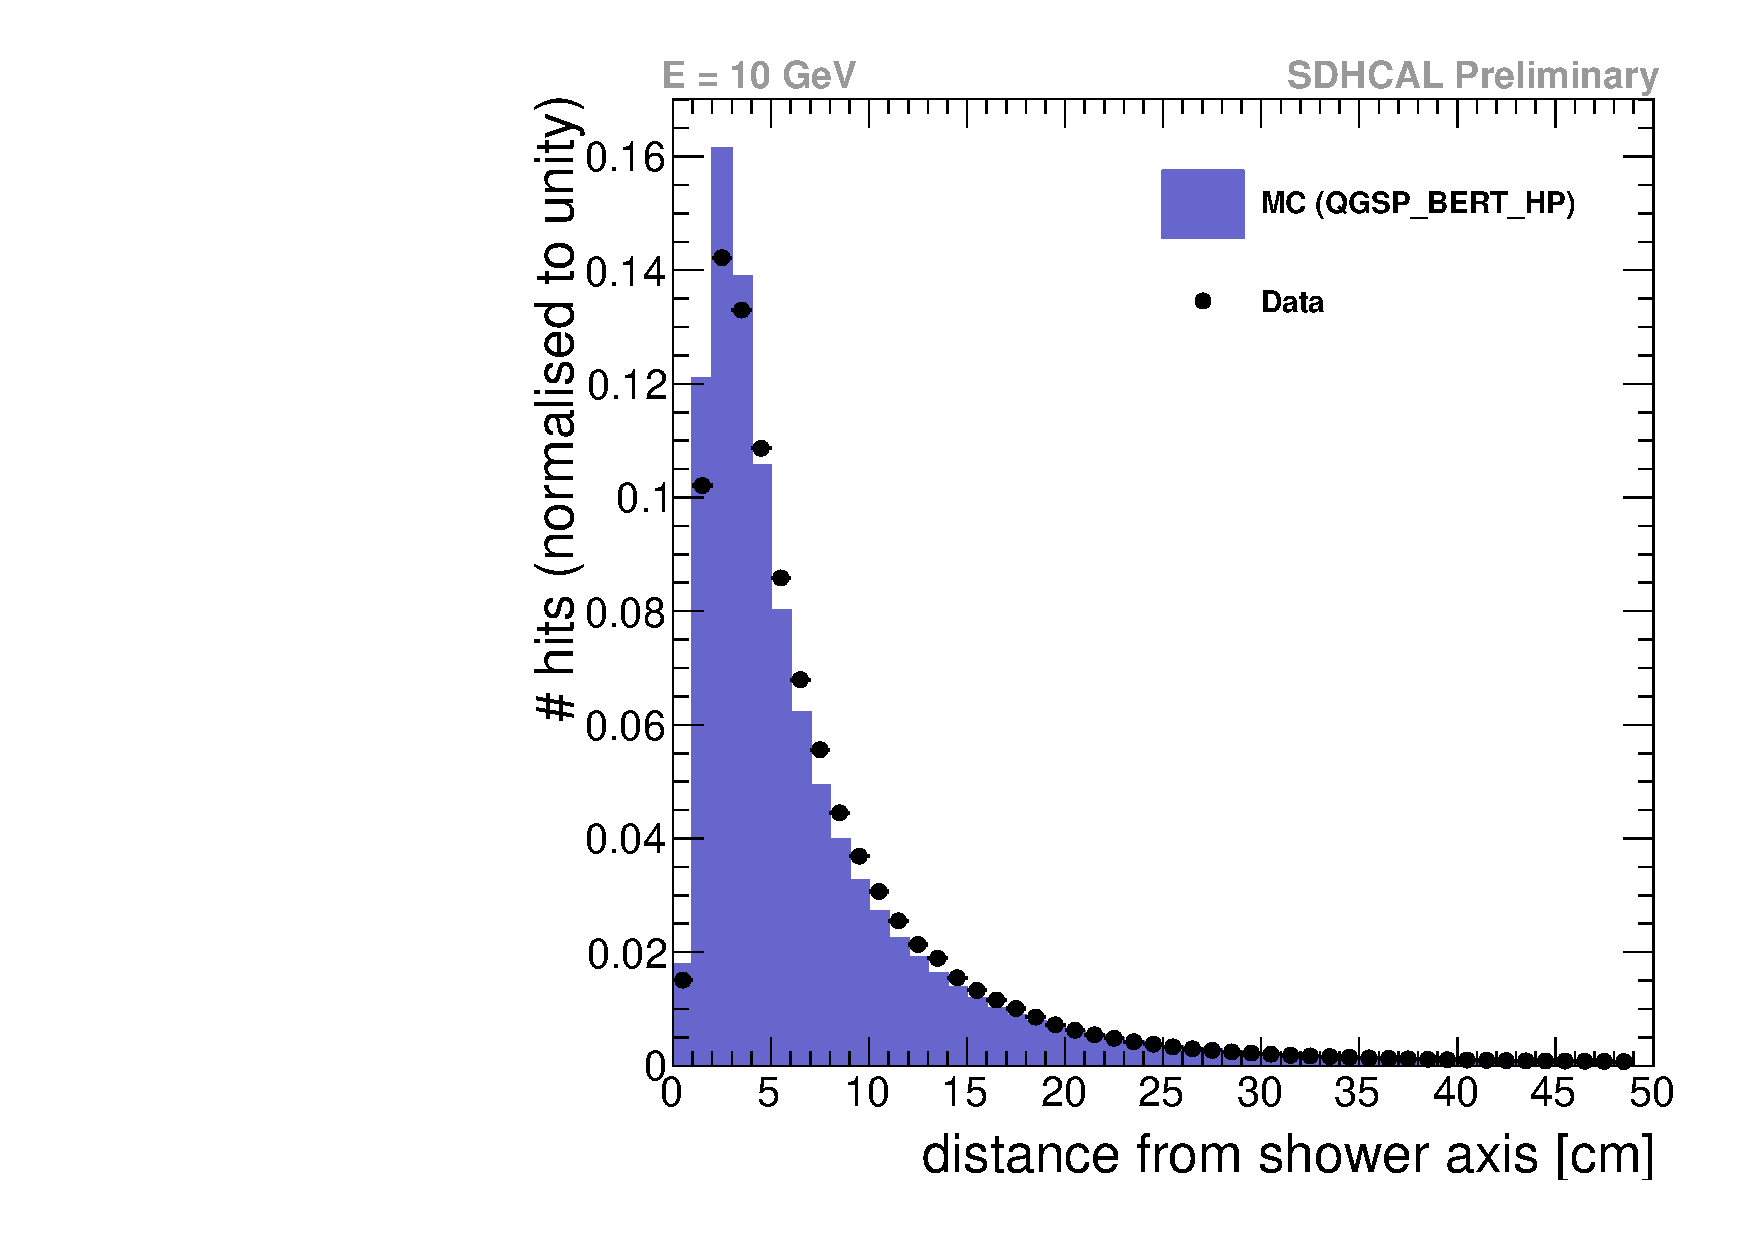
\includegraphics[width=.32\textwidth]{Shower/figs/radProf_pi-_10GeV_qgsp_bert_hp.pdf}
  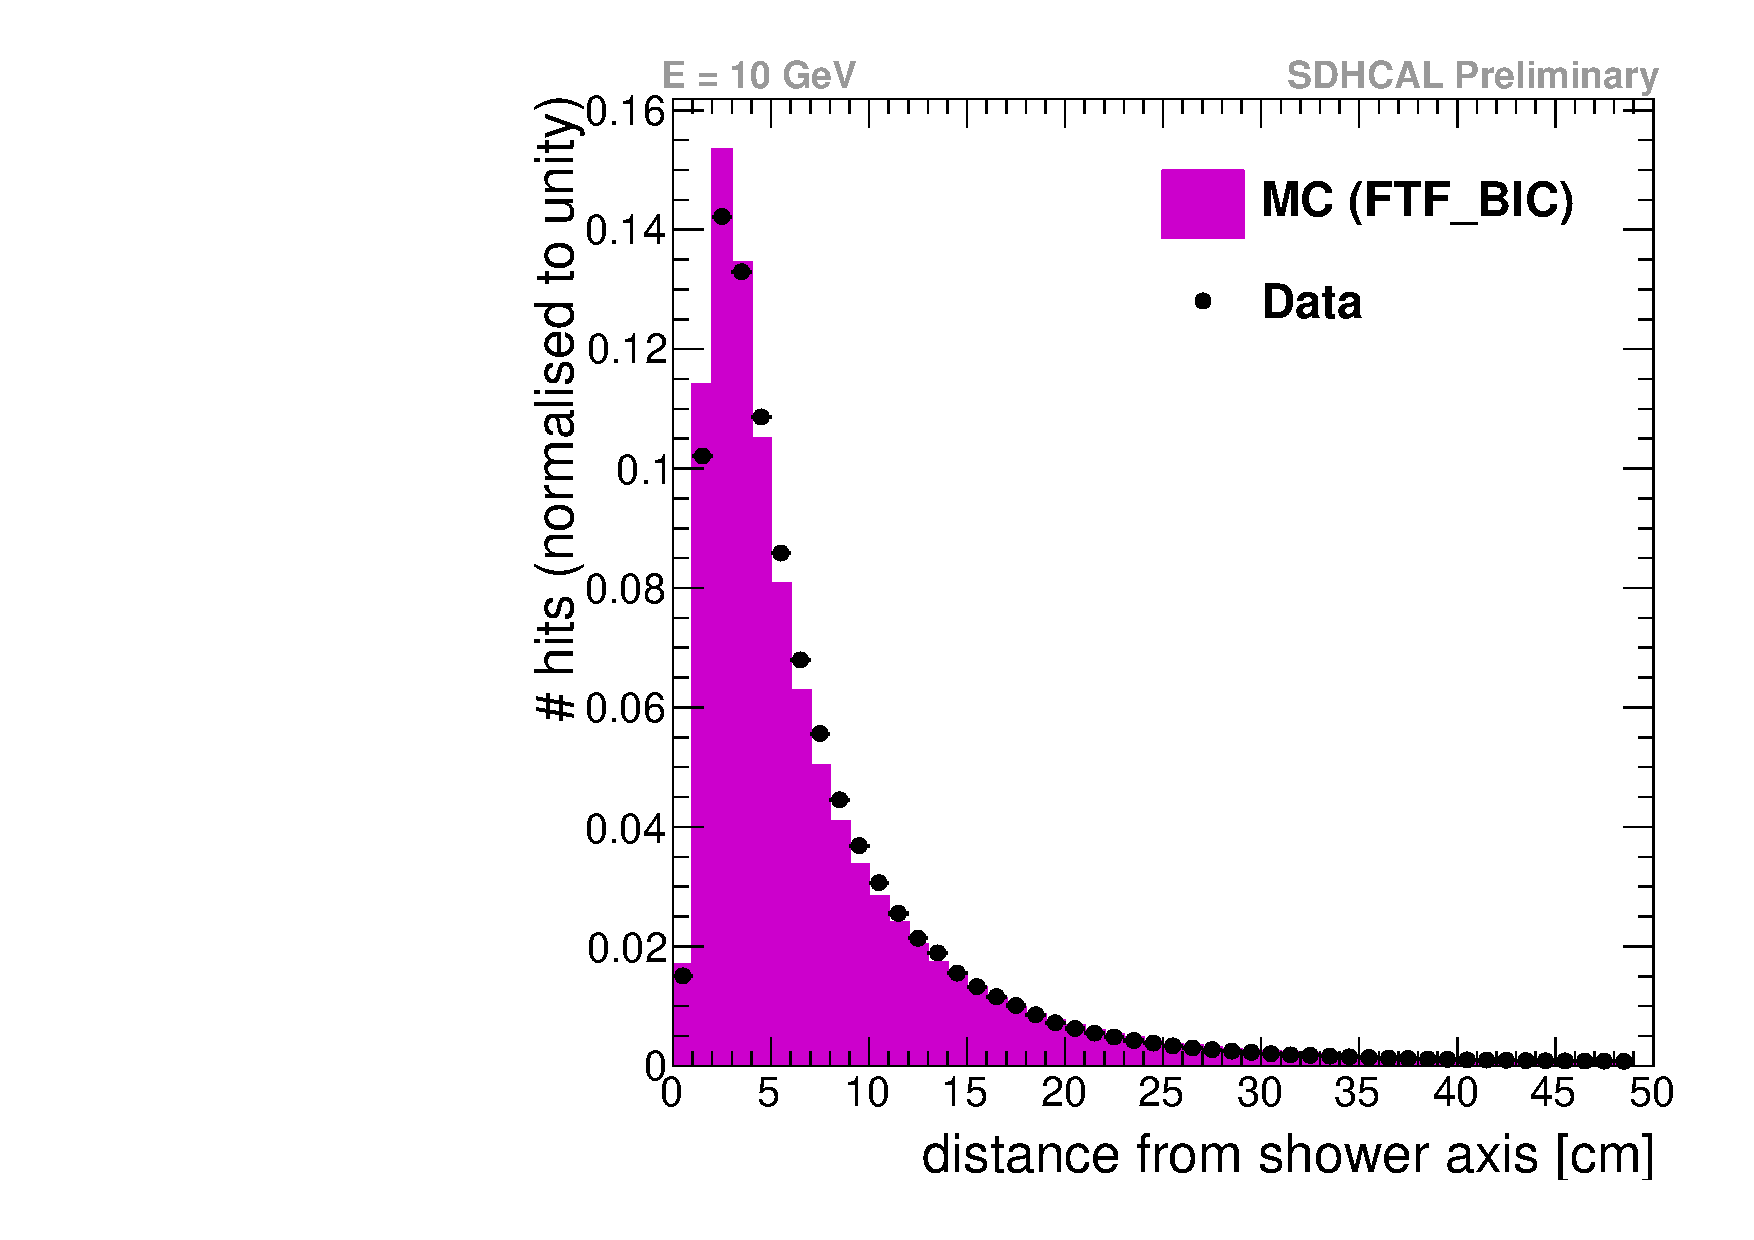
\includegraphics[width=.32\textwidth]{Shower/figs/radProf_pi-_10GeV_ftf_bic.pdf}  \\
  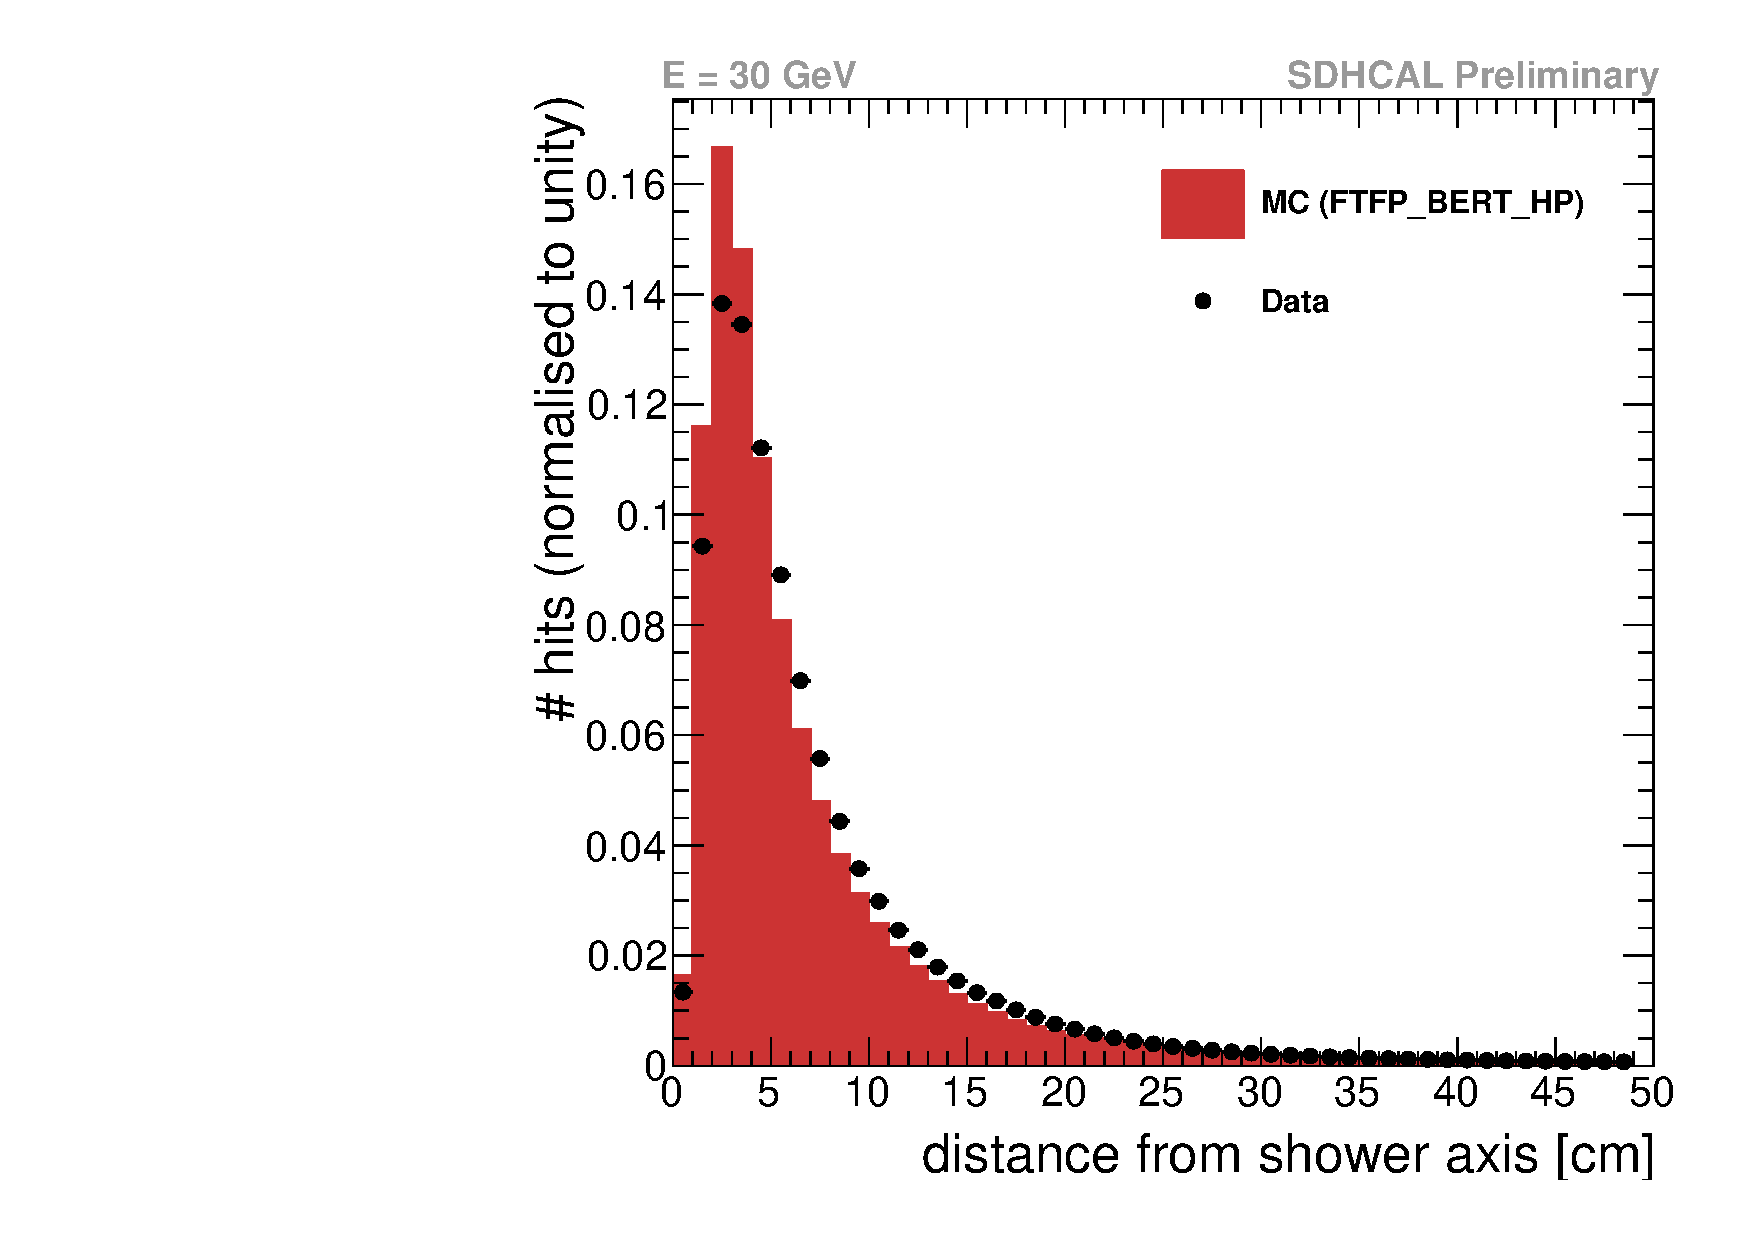
\includegraphics[width=.32\textwidth]{Shower/figs/radProf_pi-_30GeV_ftfp_bert_hp.pdf}
  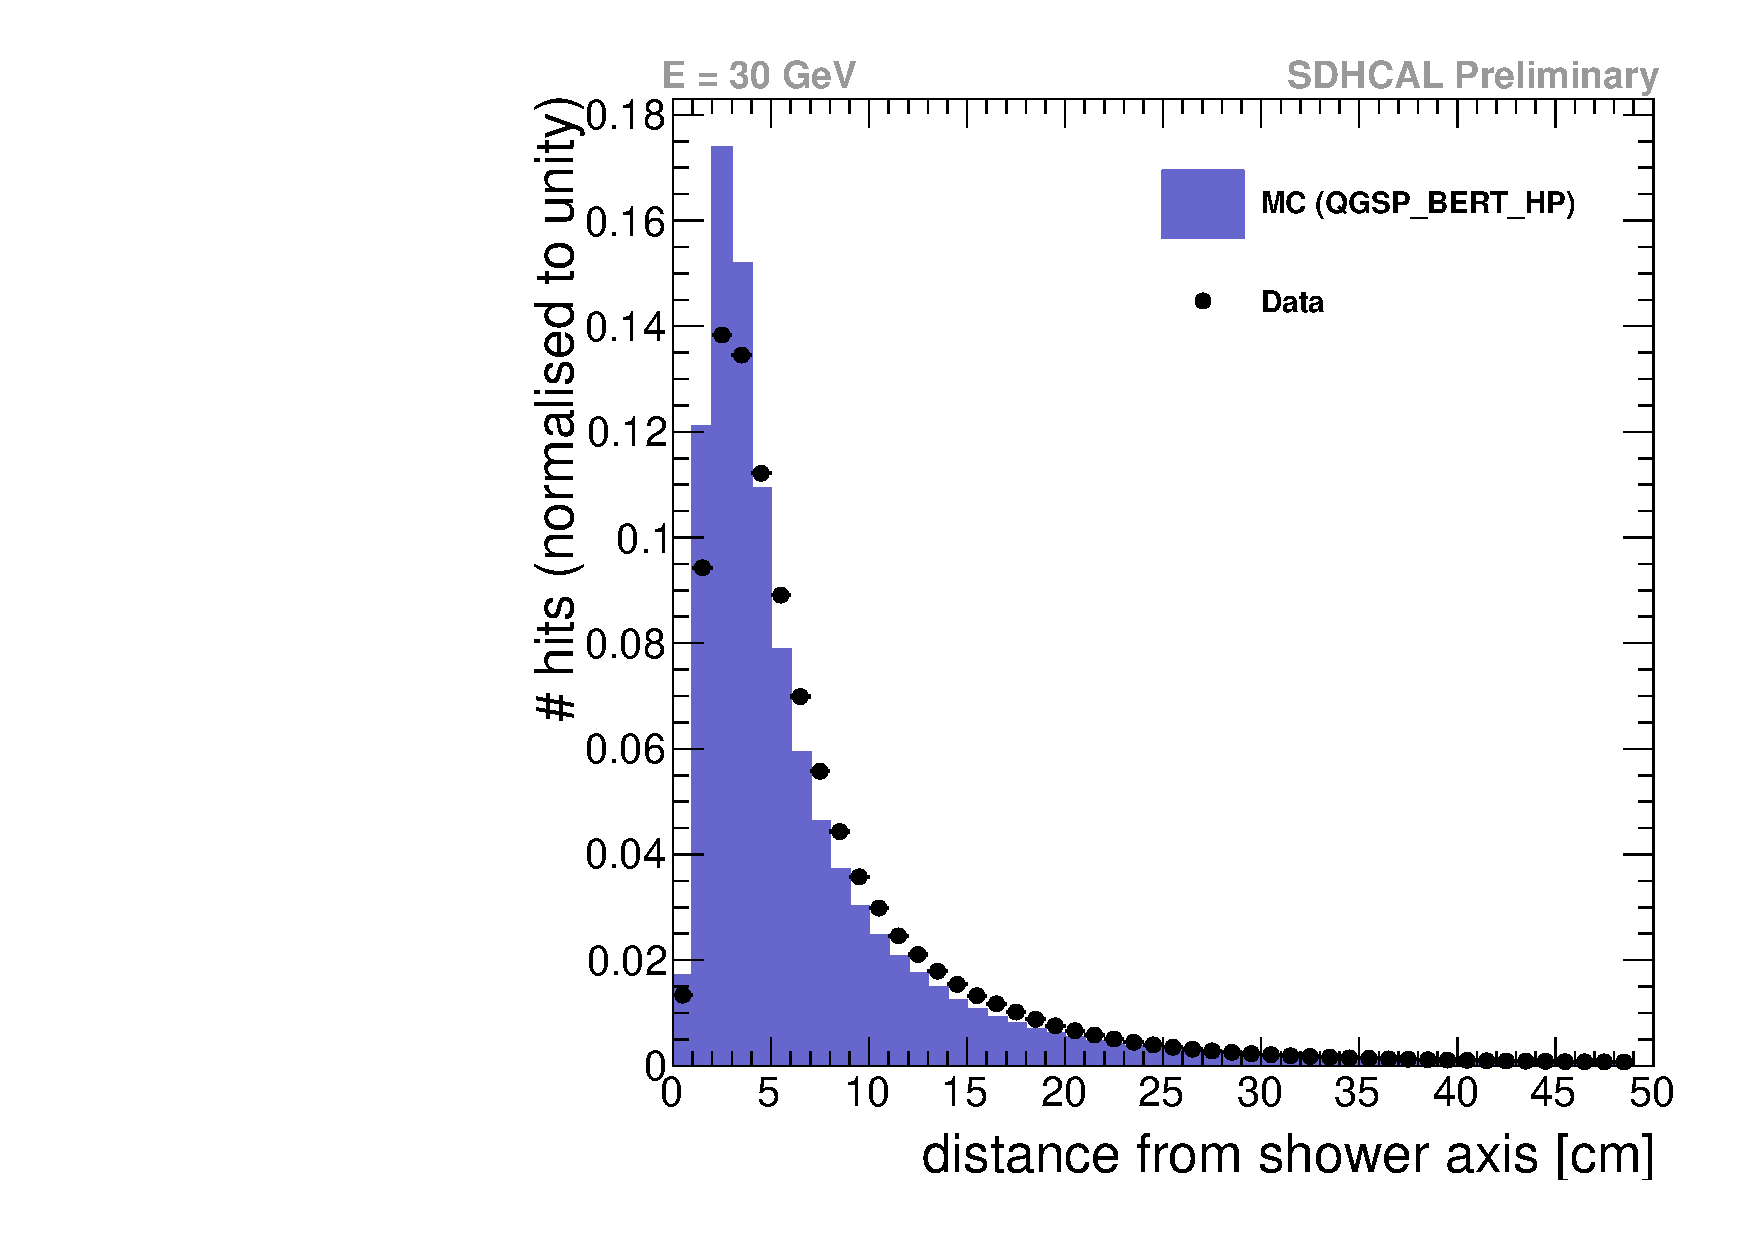
\includegraphics[width=.32\textwidth]{Shower/figs/radProf_pi-_30GeV_qgsp_bert_hp.pdf}
  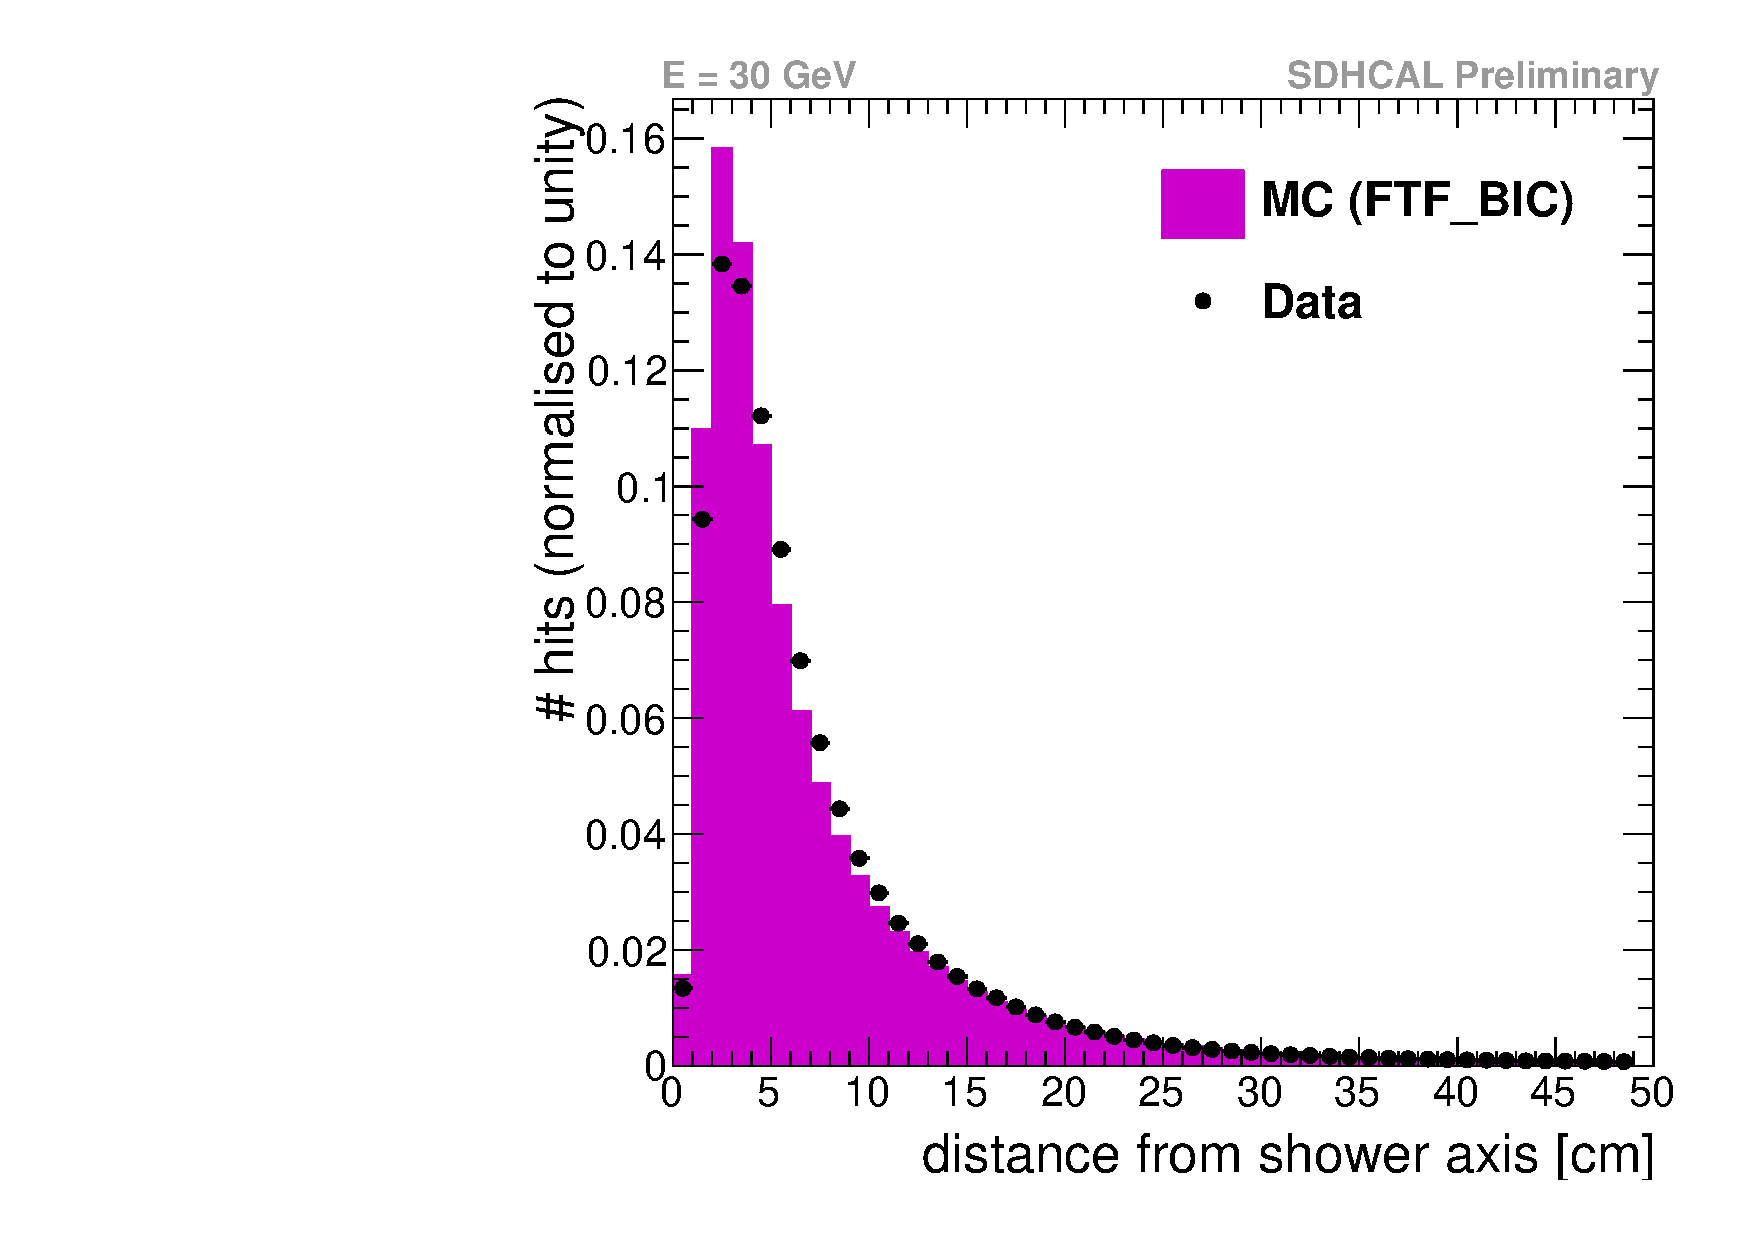
\includegraphics[width=.32\textwidth]{Shower/figs/radProf_pi-_30GeV_ftf_bic.pdf}  \\
  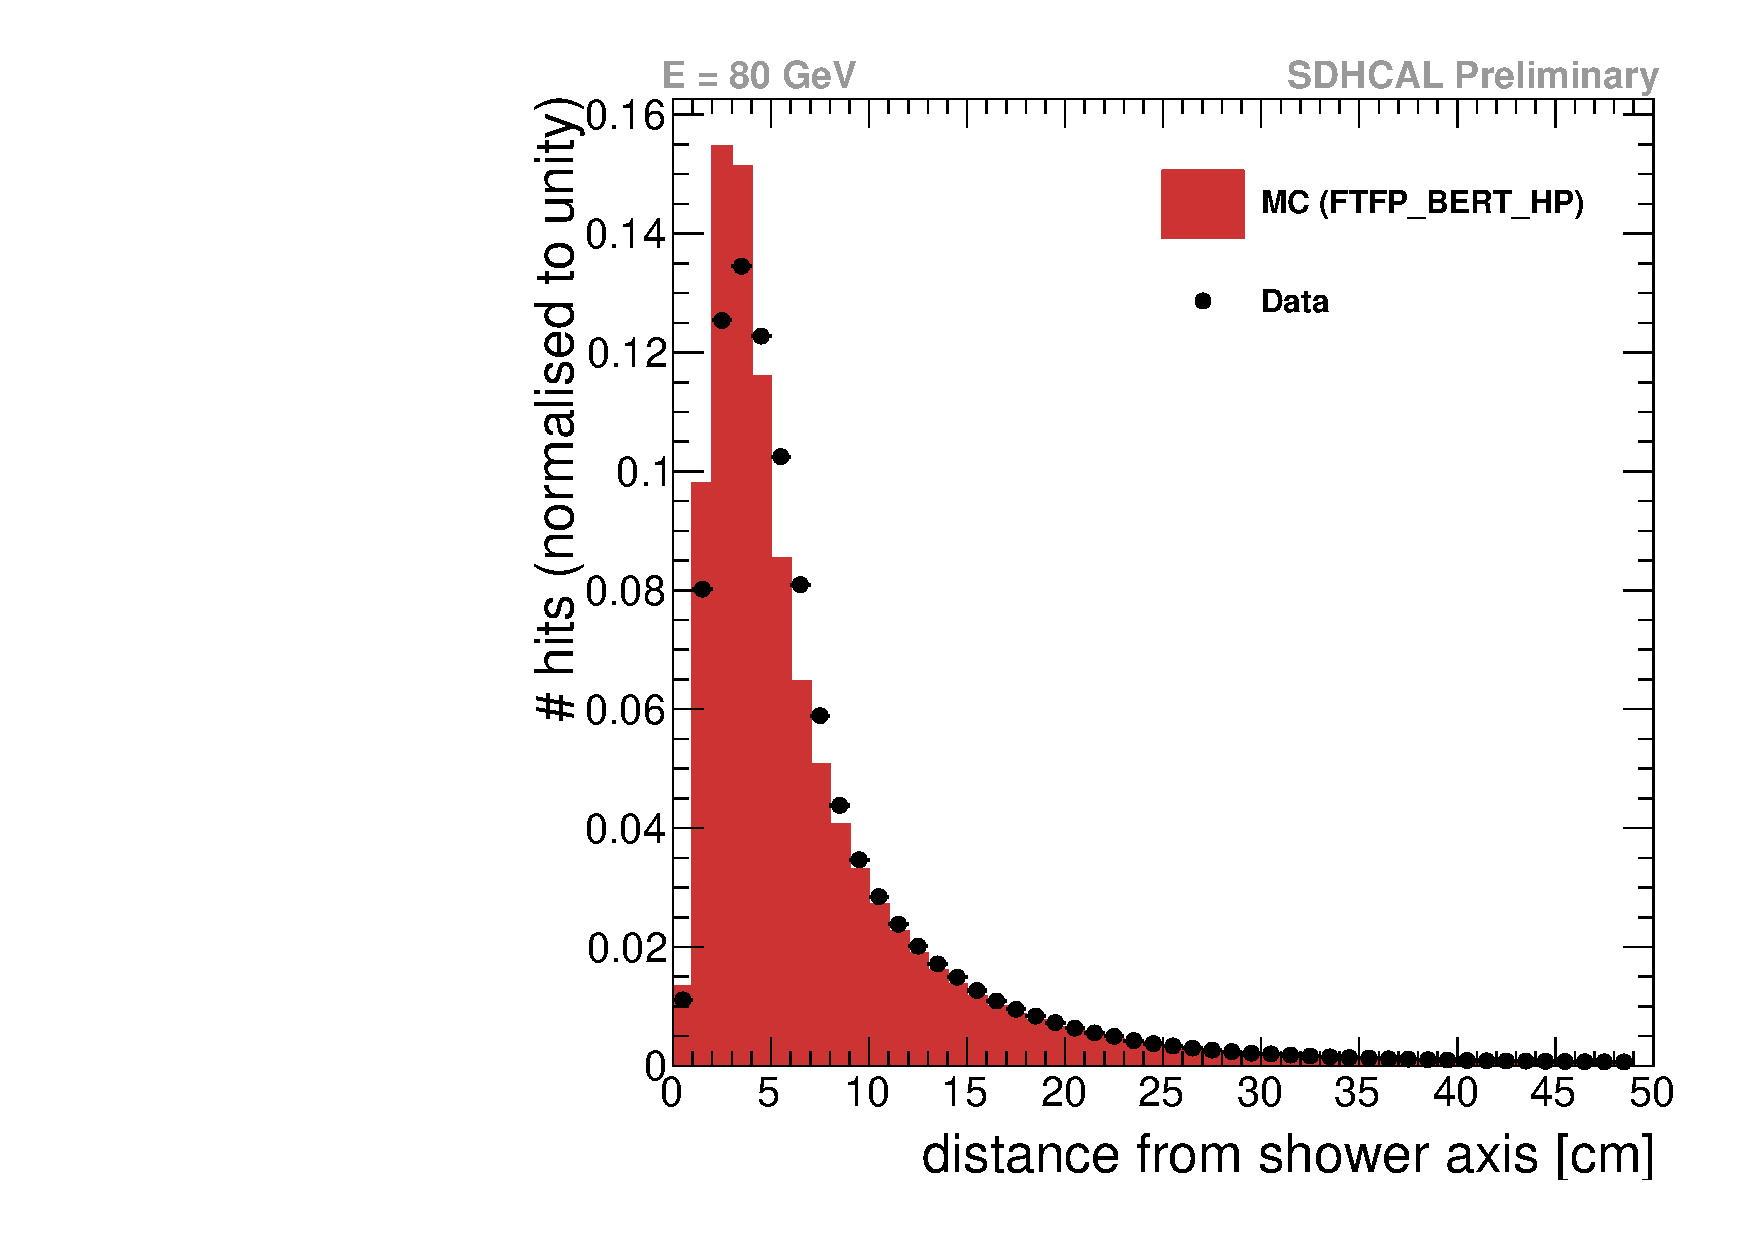
\includegraphics[width=.32\textwidth]{Shower/figs/radProf_pi-_80GeV_ftfp_bert_hp.pdf}
  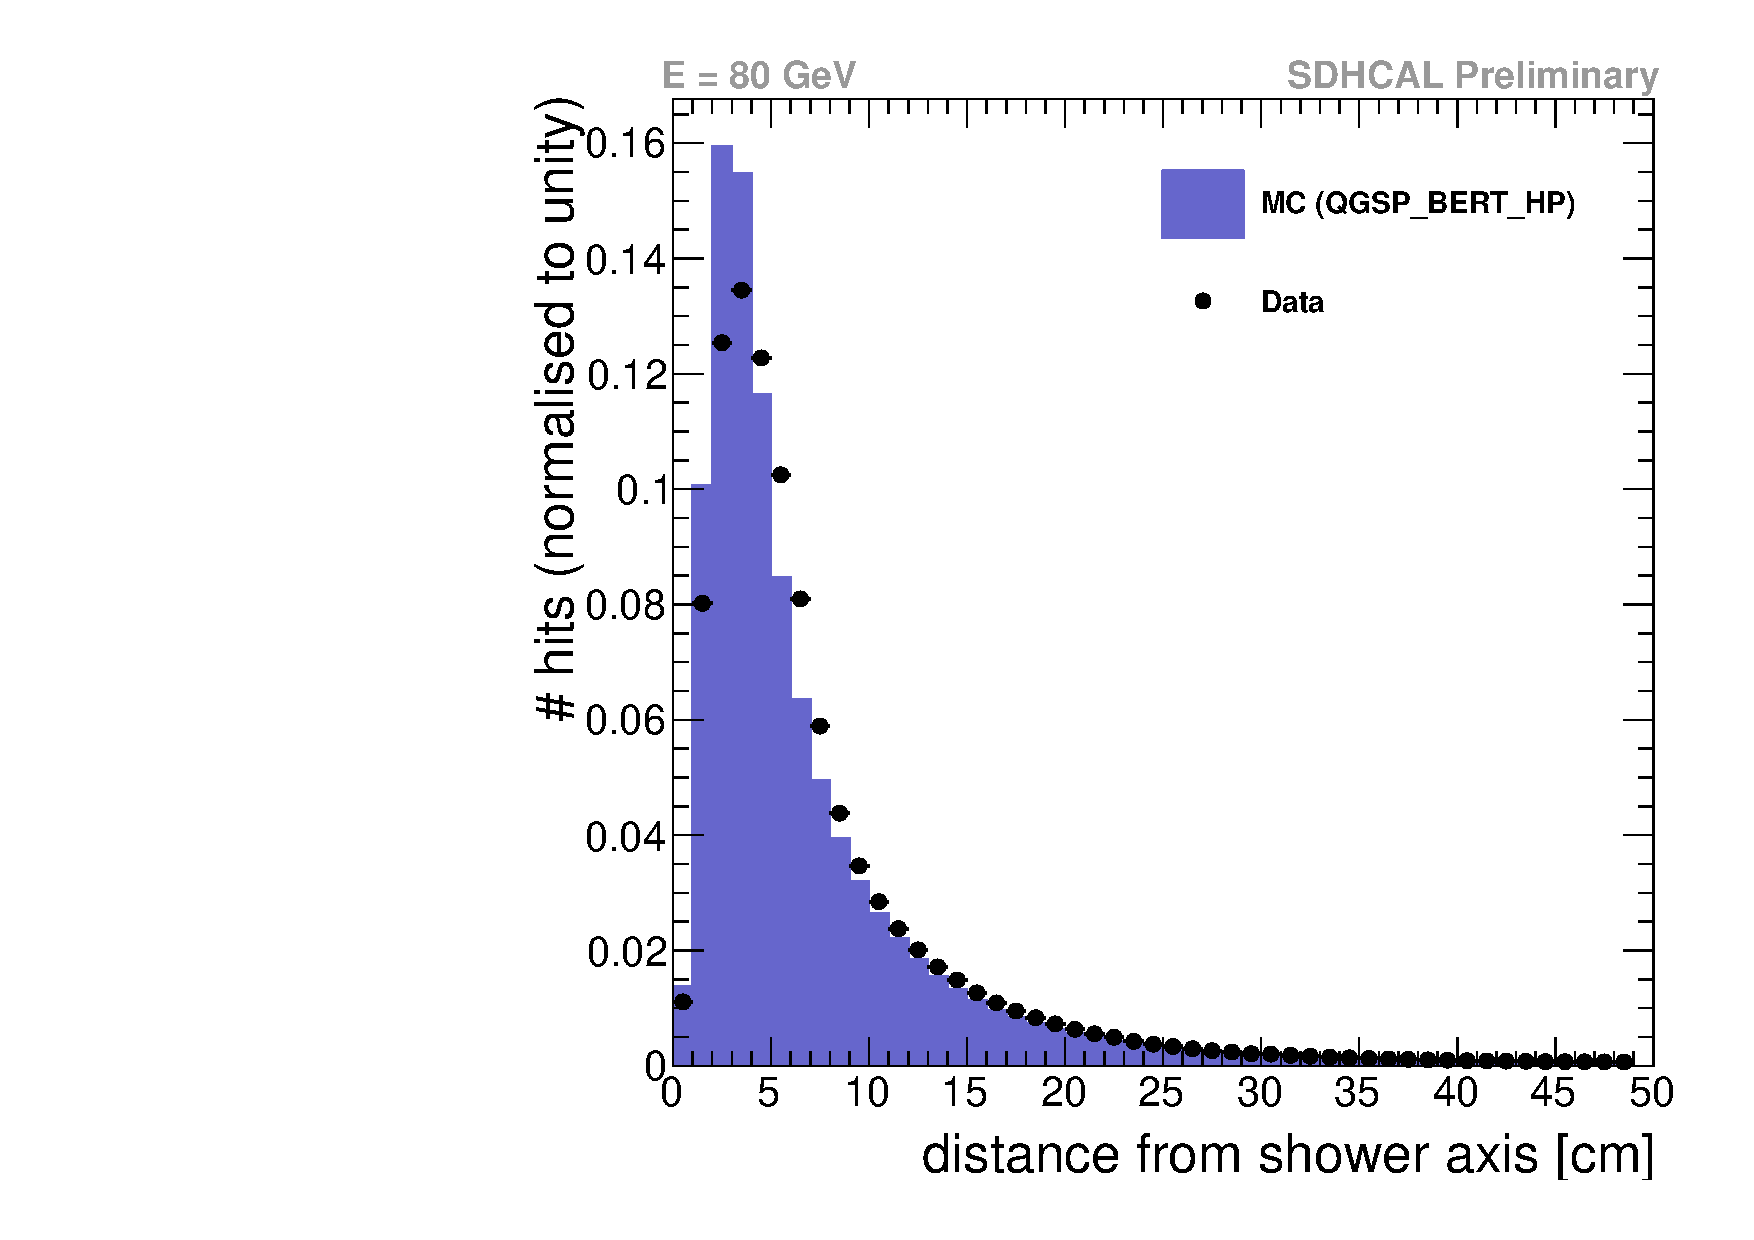
\includegraphics[width=.32\textwidth]{Shower/figs/radProf_pi-_80GeV_qgsp_bert_hp.pdf}
  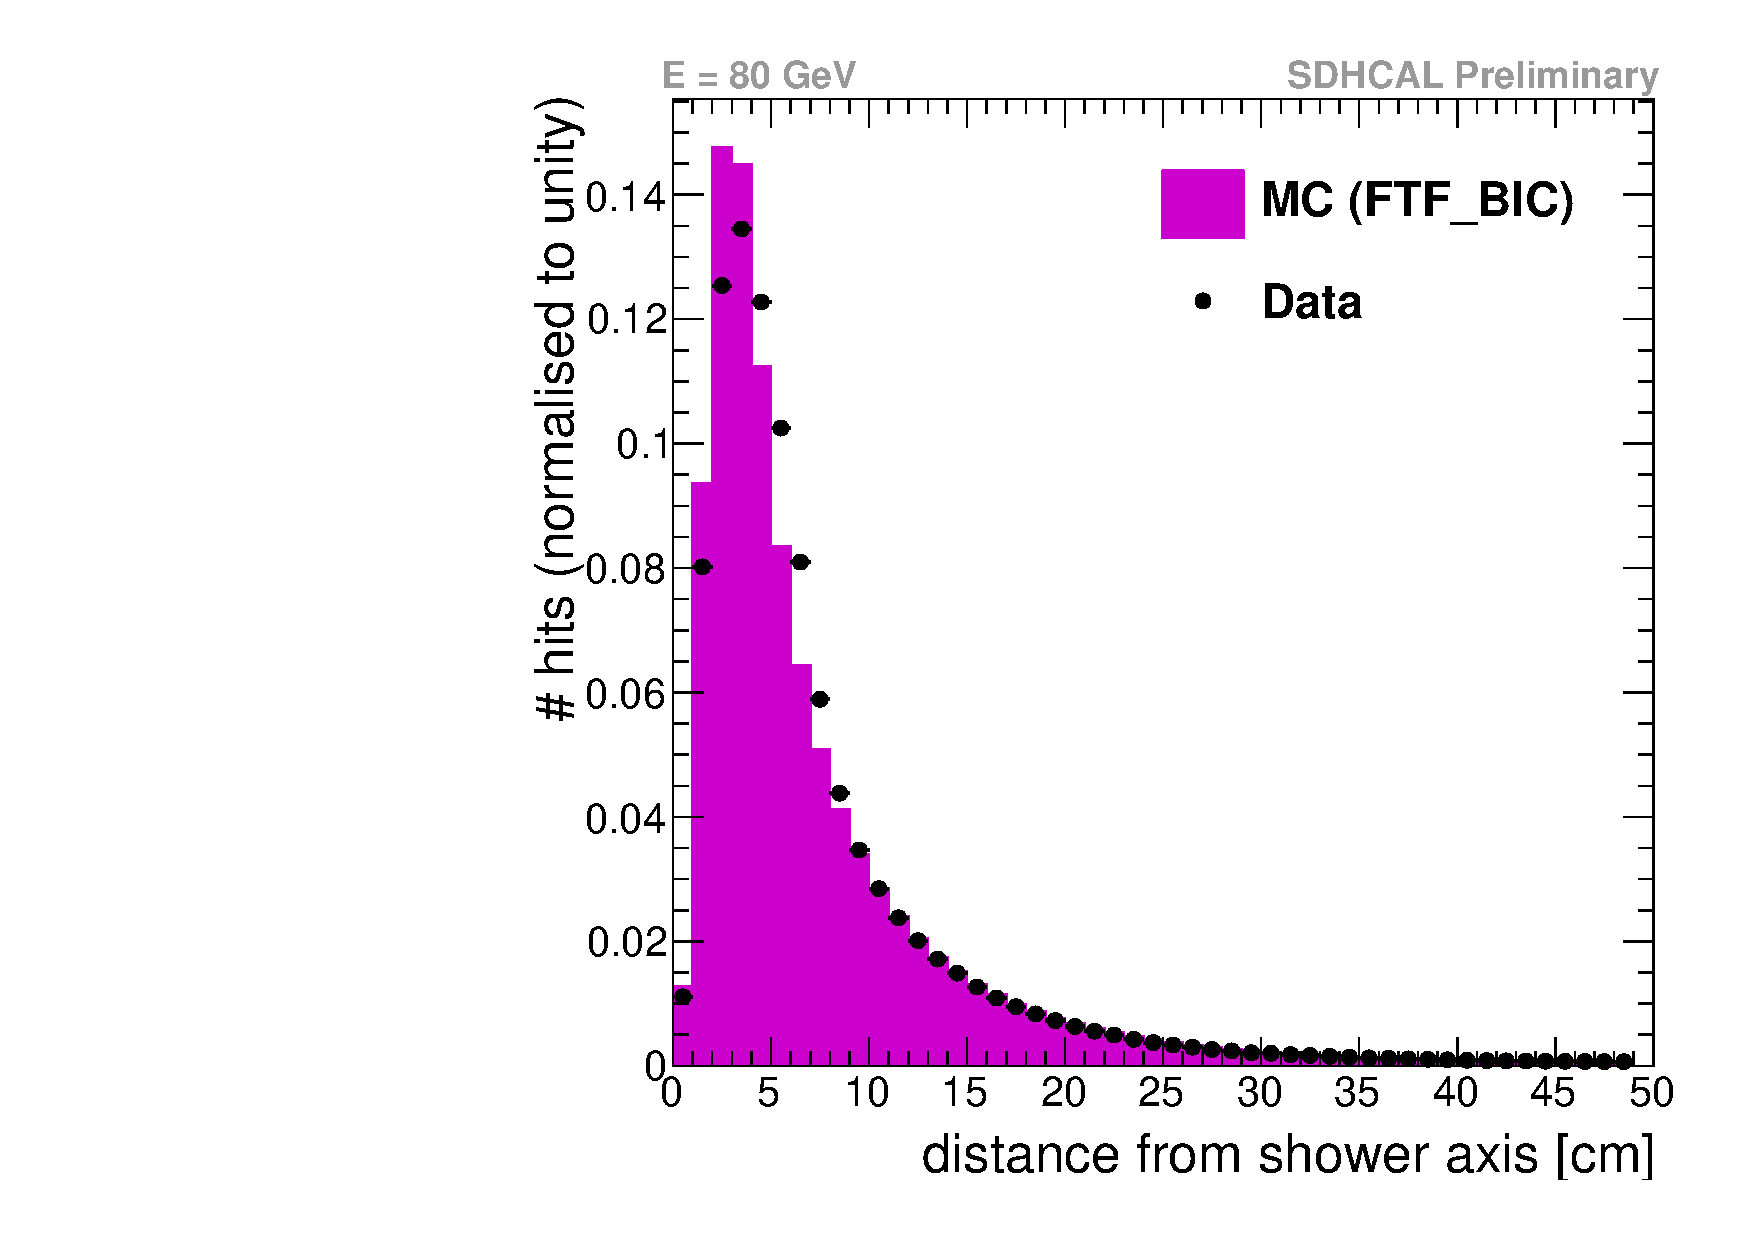
\includegraphics[width=.32\textwidth]{Shower/figs/radProf_pi-_80GeV_ftf_bic.pdf}
  \caption{Profil transversal pour des échantillons de pions de 10 GeV (en haut), de 30 GeV (au milieu) et de 80 GeV (en bas) pour les données et des simulations réalisées avec les listes FTFP\_BERT\_HP (à gauche), QGSP\_BERT\_HP (au centre) et FTF\_BIC (à droite). Les données sont représentées par des cercles noirs et la simulation par les histogrammes pleins. \label{fig.pi-radial}}
\end{figure}
Le profil latéral ou transversal est construit en comptant les cellules touchées dans des anneaux de 1 $cm$ d'épaisseur, autour de l'axe de la cascade. L'axe de la cascade est déterminé à l'aide d'une régression linéaire (cf. section~\ref{sec.pi_selection} du chapitre~\ref{chap.sdhcal}). Pour chaque cellule touchée, la distance entre l'axe de la cascade et la position de la cellule\footnote{La position d'une cellule est définie comme la position de son centre} est calculée. Selon la valeur de la distance, un compteur dans l'anneau correspondant est incrémenté. Comme pour le profil longitudinal, le nombre de hits dans chaque anneau est normalisé au nombre total de hits de l'événement puis moyenné sur tous les événements. 
%Le profil latéral correspond donc à la densité de coups moyenne en fonction de la distance à l'axe. 
Le nombre de hits par anneau est aussi corrigé en fonction du temps avec des polynômes de degré 2. La figure~\ref{fig.pi-radial} présente le profil latéral de gerbes hadroniques à 10, 30 et 80 $GeV$ pour les données et trois listes physiques. La figure~\ref{fig.pi-radial_log} de l'annexe \ref{app.radial} montre exactement les mêmes profils en base logarithmique afin de pouvoir visualiser les queues de ces profils. Pour ces trois listes physiques, le nombre de hits, au centre de la cascade ($d<4~cm$), est surestimé par rapport aux données expérimentales. Dans la région du halo~($d\geq4~cm$ et $d<20~cm$), la simulation le sous-estime. Les queues des profils sont raisonnablement bien simulées même si, pour la liste FTF\_BIC, le nombre de hits dans la queue semble légèrement plus élevé que dans les données (voir la figure~\ref{fig.pi-radial_log} en base logarithmique). Ceci est probablement dû à l'absence du modèle de haute précision pour les neutrons. Notons que la coupure à 1000 $ns$, sur le temps d'occurence des segments dans les couches de gaz (cf. section~\ref{sec.algo} du chapitre~\ref{chap.simulation}), permet d'améliorer significativement la description de ces queues de profil. La valeur moyenne des profils transversaux est donnée par:
\begin{equation}
  <R>=\frac{1}{N_{event}}\sum_{i=0}^{N_{event}}\sum_{r=0}^{R_{max}}r\frac{N_{r,i}}{N_{tot,i}}
\end{equation}
où $N_{event}$ est le nombre d'événements, $N_{r,i}$ le nombre de cellules touchées dans l'anneau de rayon $r$ pour l'événement $i$ et $N_{tot,i}$ le nombre total de hits pour l'événement $i$. $R_{max}$ correspond à la distance maximum possible entre une cellule touchée et l'axe de la cascade ($\sqrt{2}~m$ pour le prototype du SDHCAL).

\begin{figure}[!ht]
  \centering
  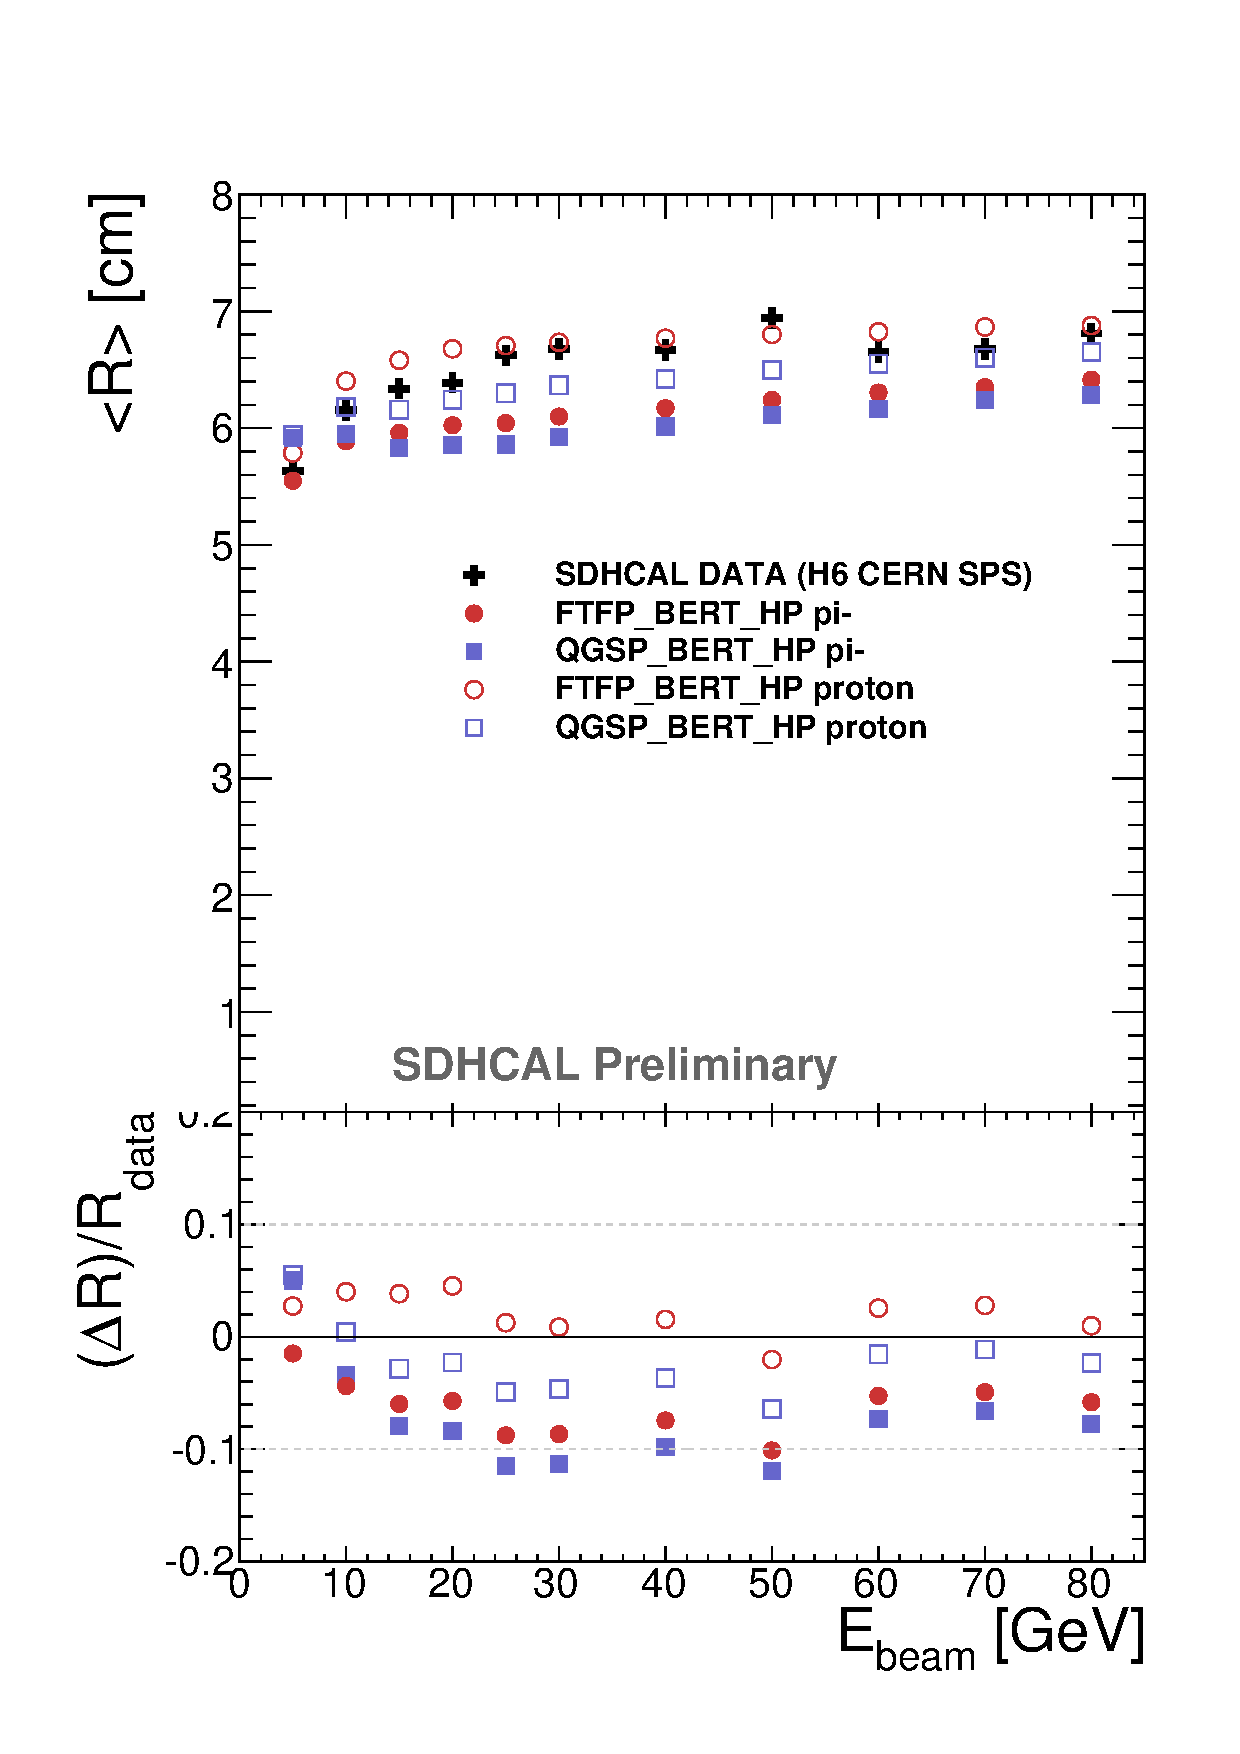
\includegraphics[width=.48\textwidth]{Shower/figs/RADPIONHP.pdf}
  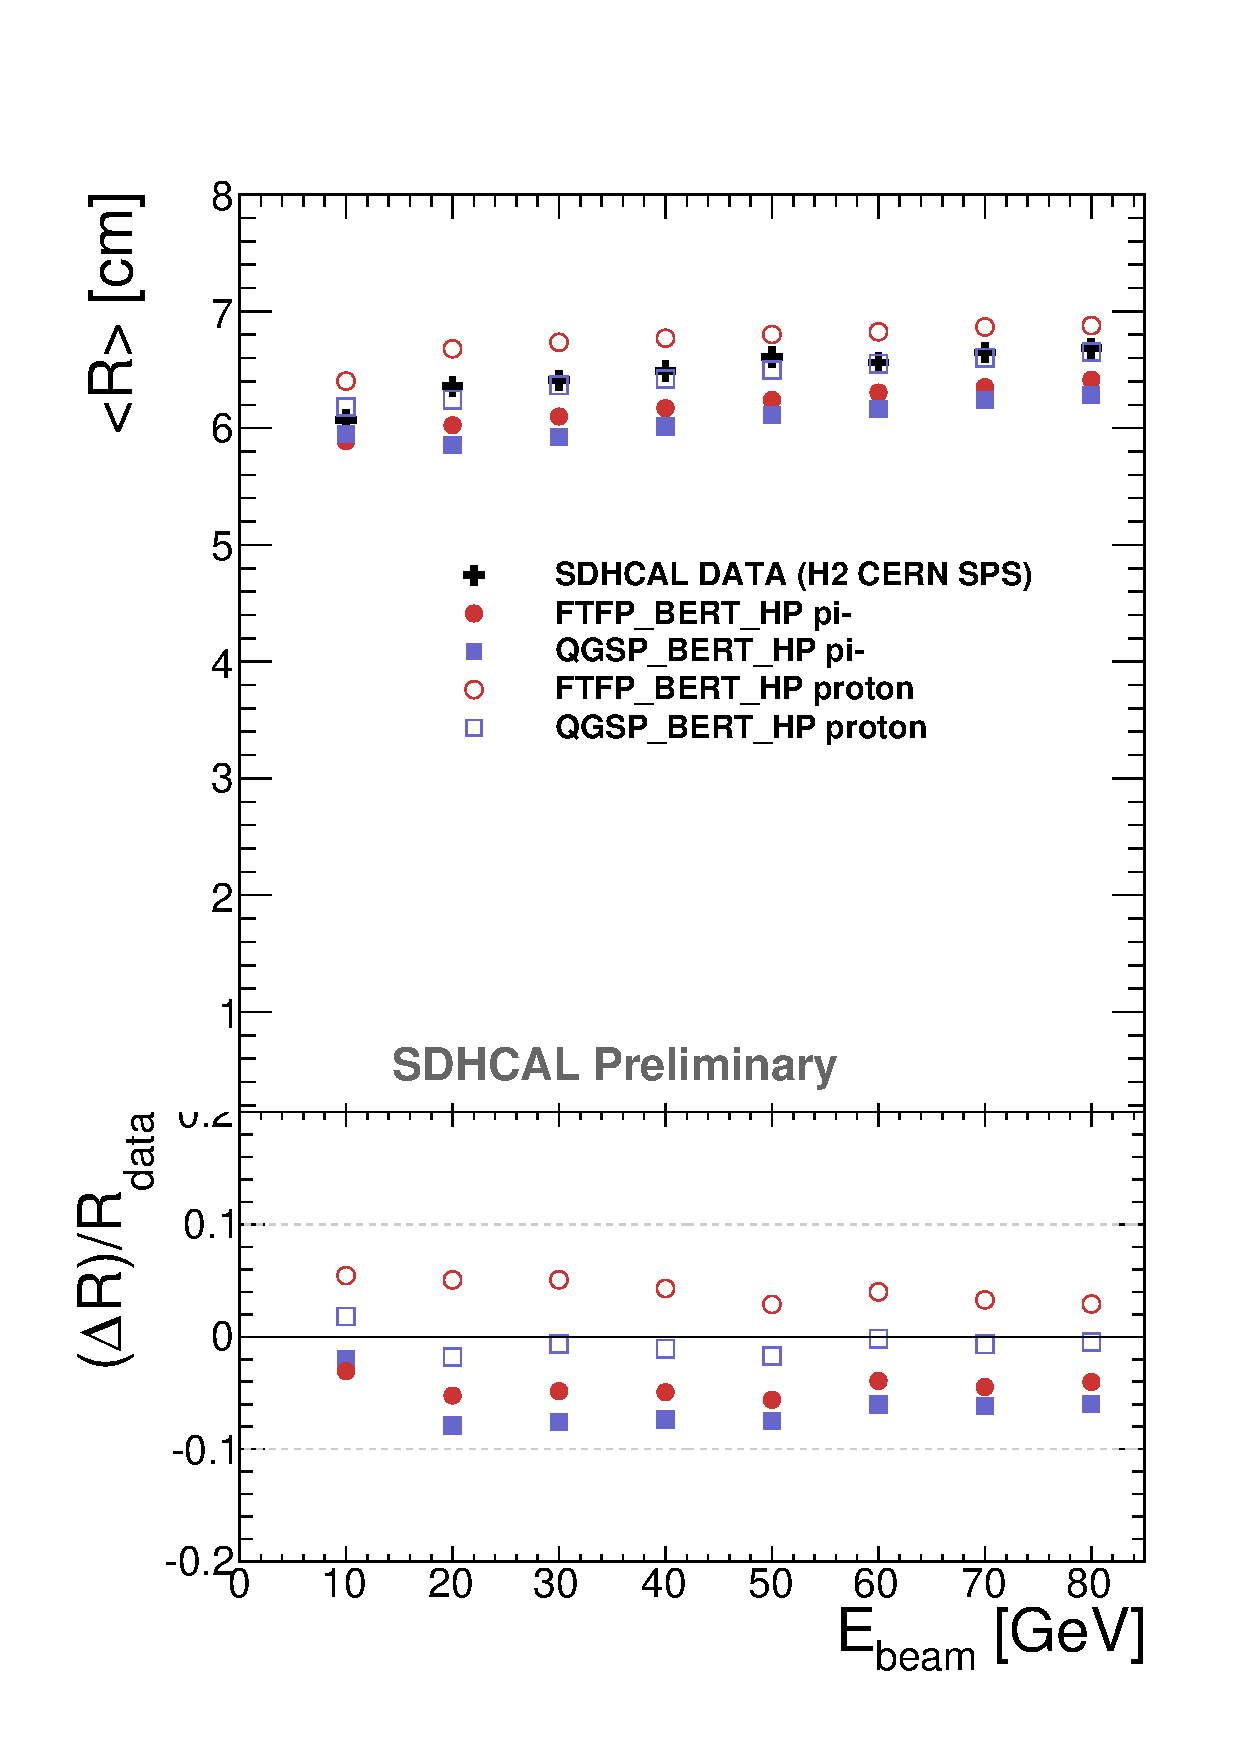
\includegraphics[width=.48\textwidth]{Shower/figs/RADPIONNOV.pdf}
  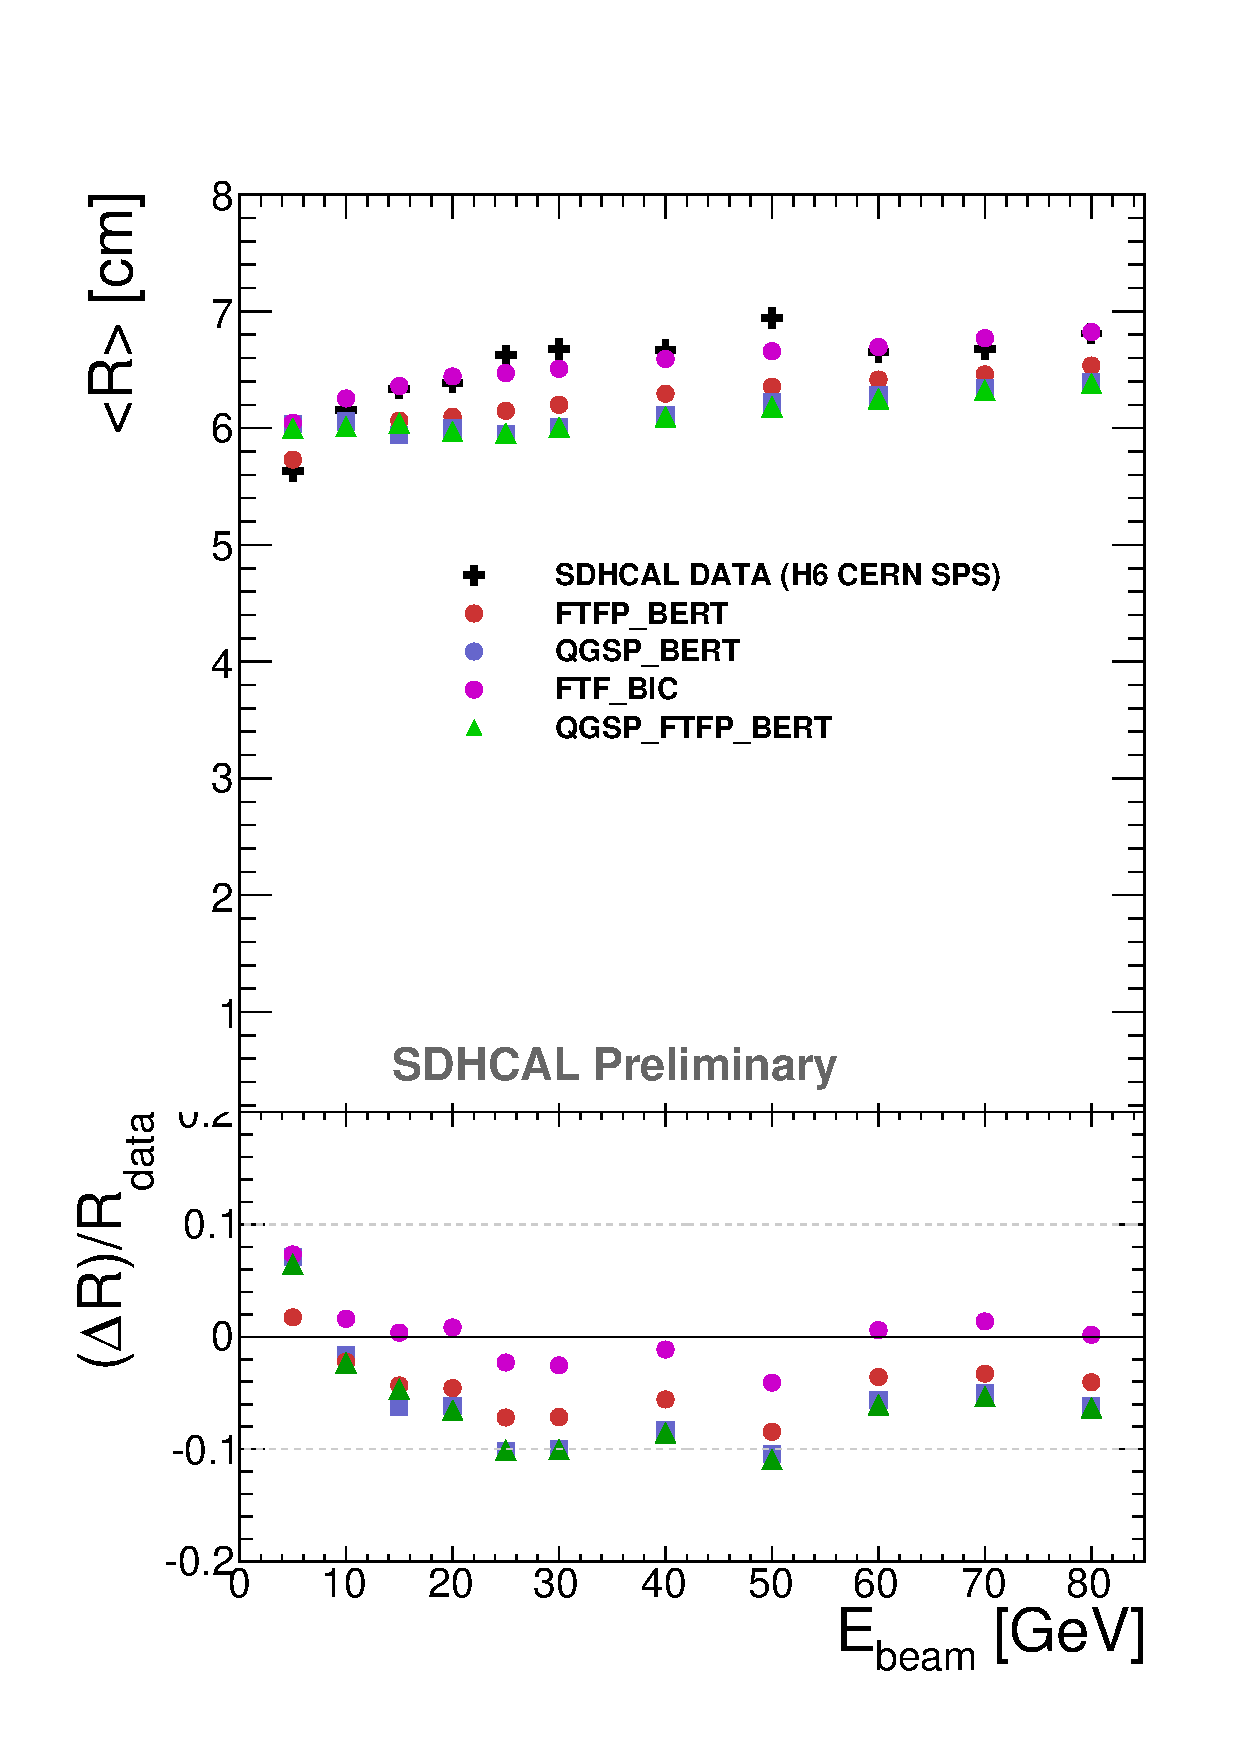
\includegraphics[width=.48\textwidth]{Shower/figs/RADPROF_PION_MODEL.pdf}
  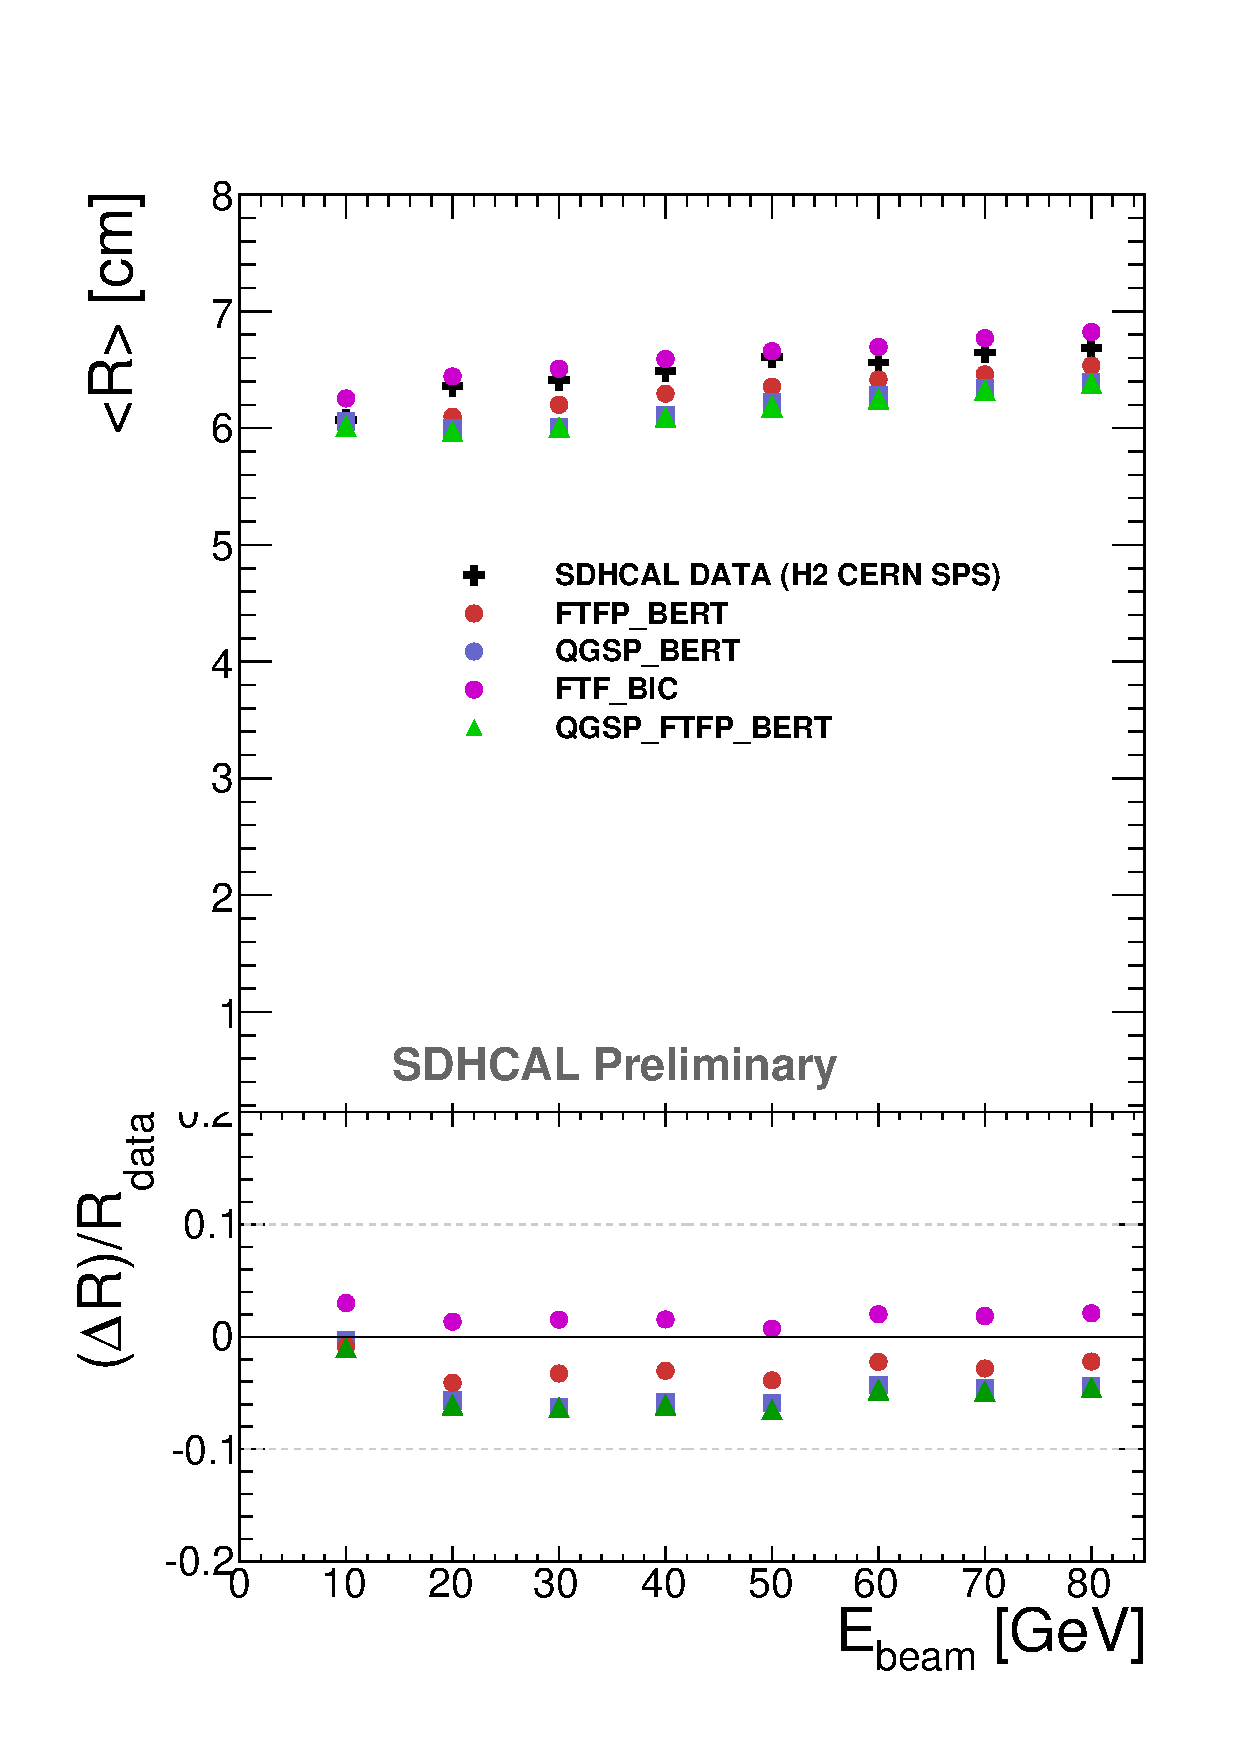
\includegraphics[width=.48\textwidth]{Shower/figs/RADPROF_PION_MODEL_NOV.pdf}
  \caption{Valeur moyenne et déviation relative du profil latéral en fonction de l'énergie du faisceau pour les données enregistrées sur la ligne H6 (à gauche) et H2 (à droite) et plusieurs listes physiques. Les figures du haut montrent aussi les résultats pour des simulations initiées par des protons. La taille des barres d'erreurs est inférieure à celle des points.}
  \label{fig.radial_pi-_ebeam}
\end{figure}
La figure~\ref{fig.radial_pi-_ebeam} montre la valeur moyenne du profil latéral en fonction de l'énergie du faisceau pour les données et plusieurs listes physiques. La déviation relative est définie par $\frac{<R_{simu}>-<R_{data}>}{<R_{data}>}$. Comme pour l'extension longitudinale, l'extension latérale est plus élevée pour les gerbes hadroniques initiées par des protons que par des pions. La plupart des listes physiques sous-estiment légèrement l'extension latérale des gerbes hadroniques. Les listes physiques utilisant le modèle de Fritiof pour les interactions de haute énergie présentent un meilleur accord avec les données expérimentales et la liste FTF\_BIC est celle qui les reproduit le mieux.

\begin{figure}[!ht]
  \subfigure[]{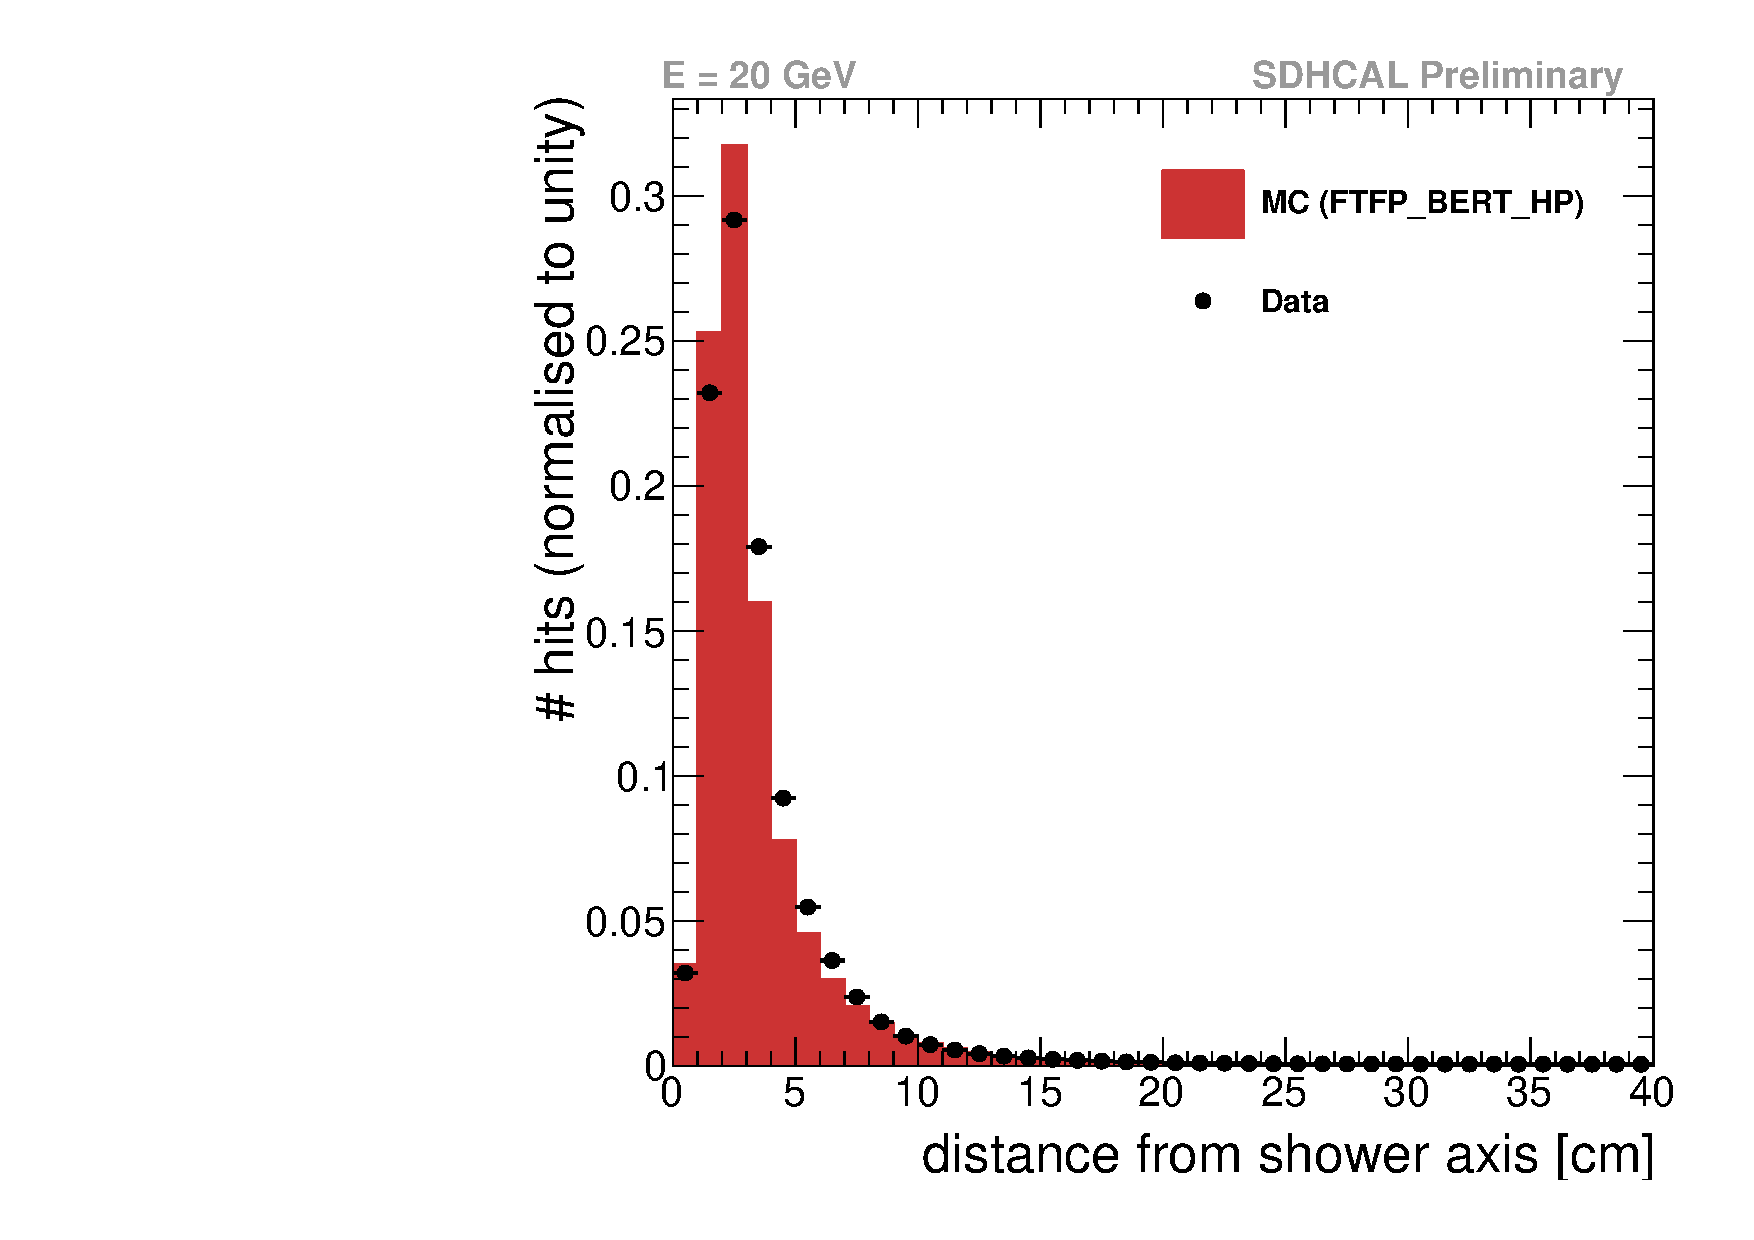
\includegraphics[width=.48\textwidth]{Shower/figs/radProf_e-_20GeV_AugSep2012.pdf}}
  \subfigure[]{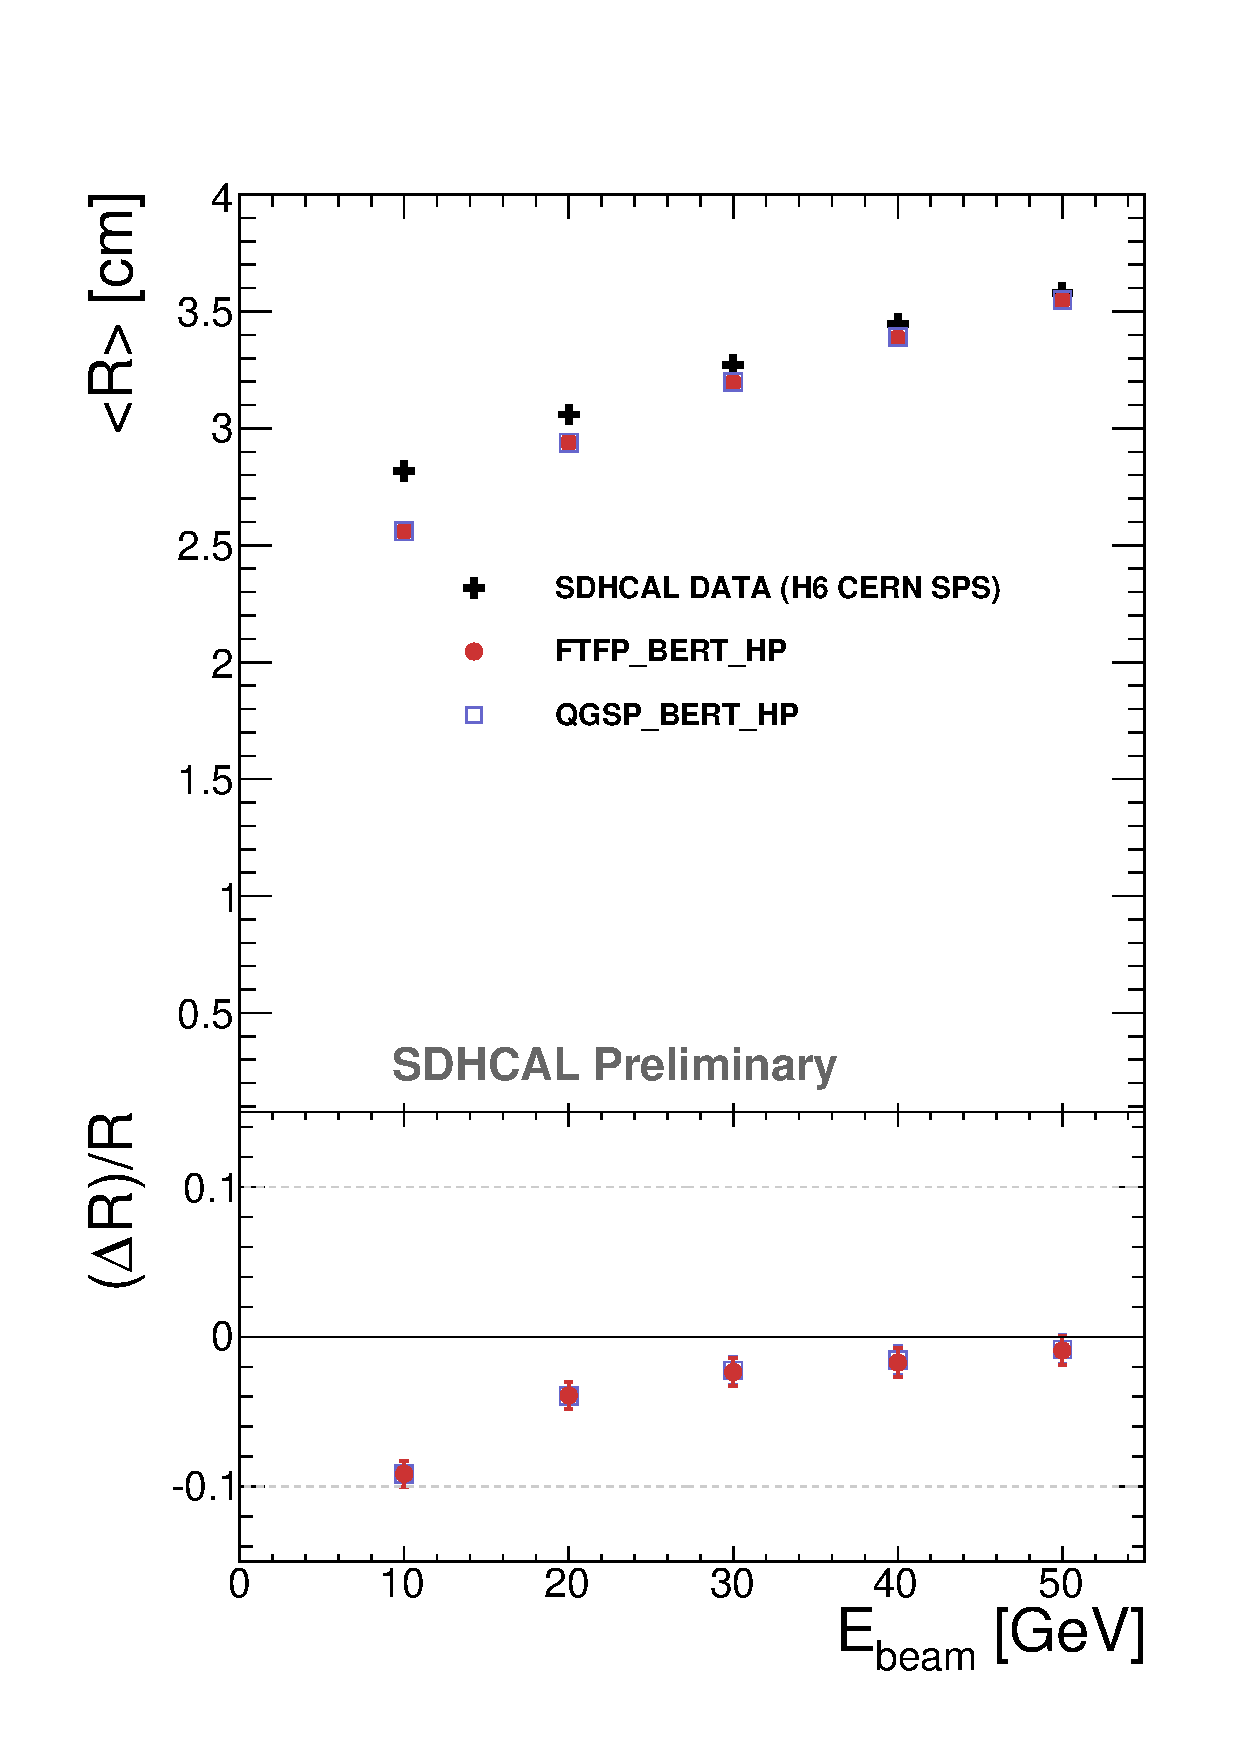
\includegraphics[width=.4\textwidth]{Shower/figs/RADELECTRON.pdf}}
  \caption{(a): Profil latéral de gerbes électromagnétiques à 20 $GeV$ pour les données (cercles noirs) et une simulation réalisée avec la liste physique FTFP\_BERT\_HP (histogramme rouge). (b) Valeur moyenne et déviation relative du profil latéral pour des gerbes électromagnétiques en fonction de l'énergie du faisceau.}
  \label{fig.rad_e-}
\end{figure}
La figure~\ref{fig.rad_e-}(a) présente le profil latéral des gerbes électromagnétiques de 20 $GeV$ pour les données et un échantillon de simulation (FTFP\_BERT\_HP). La valeur moyenne et la déviation relative en fonction de l'énergie du faisceau est donnée par la figure~\ref{fig.rad_e-}(b). La simulation est en accord avec les données au dessus de 30 $GeV$. A plus basse énergie, la simulation sous-estime légèrement l’extension latérale des gerbes électromagnétiques. Des études systématiques sur les coupures de sélection des gerbes électromagnétiques, et sur le bruit dans les données, n'ont pas permis d'expliquer ces différences.

Les résultats obtenus sur le profil latéral des gerbes hadroniques permettent de justifier ceux obtenus dans le chapitre précédent. Ils montraient des désaccords entre la simulation et les données sur la réponse du SDHCAL aux gerbes hadroniques. La liste physique FTF\_BIC, qui montrait le meilleur accord avec les données sur le nombre de hits, est aussi la meilleure pour décrire l'extension latérale des gerbes hadroniques. Le profil latéral des gerbes hadroniques a aussi été étudié par le calorimètre CALICE AHCAL. La conclusion de cette étude était que l'extension latérale des gerbes hadroniques était sous-estimée par la simulation \cite{geant4-ahcal}. Comme pour les autres variables, les premiers tests avec la version 10.1 de GEANT4 ne montrent pas de changement notable pour le profil latéral des gerbes hadroniques. 
%Enfin, dans le chapitre~\ref{chap.sdhcal}, nous avons mentionné qu'un problème dans le modèle de Fritiof a été corrigé à partir de la version 10.1 de GEANT4. Cette correction devrait diminuer l'extension des gerbes hadroniques et aggraver les différences entre les données et les simulations basées sur le modèle de Fritiof.
%%%%%%%%%%%%%%%%%%%%%%%%%%%%%%%%%%%%%%%%%%%%%%%

\section{Reconstruction des traces dans le SDHCAL}
\label{sec.hough}
Nous avons vu dans le chapitre~\ref{chap.shower} que de nombreuses particules sont créées dans une gerbe hadronique. Les interactions possibles de ces particules avec la matière sont souvent multiples. Certaines particules chargées traversent une quantité plus ou moins importante de matière en ne déposant de l'énergie que par ionisation. Avec un détecteur suffisamment segmenté comme le SDHCAL, il est possible de reconstruire la trajectoire de ces particules. Ces traces pourraient permettre d'améliorer la reconstruction de l'énergie (cf. section~\ref{sec.ereco} du chapitre~\ref{chap.sdhcal}), et de surveiller le comportement et les performances (efficacité, multiplicité) du détecteur {\it{in situ}}. La reconstruction de ces traces pourrait aussi être utile dans les algorithmes de suivi de particules (PFA): association d'une trace primaire (avant la première interaction inélastique) avec une trace reconstruite dans le trajectographe, association de dépôts hadroniques etc. Ces segments peuvent aussi être utilisés pour la comparaison des modèles de simulation avec les données. Une méthode de reconstruction des traces utilise la Transformée de Hough \cite{houghPatent} qui a été développée en 1962, pour détecter des lignes et arcs de cercles dans des chambres à brouillard. Cette méthode permet d'identifier des lignes dans un environnement bruyant comme, par exemple, les gerbes hadroniques. Cette méthode a déjà été mise en œuvre avec le calorimètre électromagnétique CALICE Si-W \cite{can023} où la méthode a montré son efficacité pour identifier des muons proches de gerbes électromagnétiques. Cette étude montrait aussi que la reconstruction des traces permet de discriminer les gerbes électromagnétiques et hadroniques de façon efficace.
\subsection{La méthode de Transformée de Hough}
\begin{figure}[!ht]
  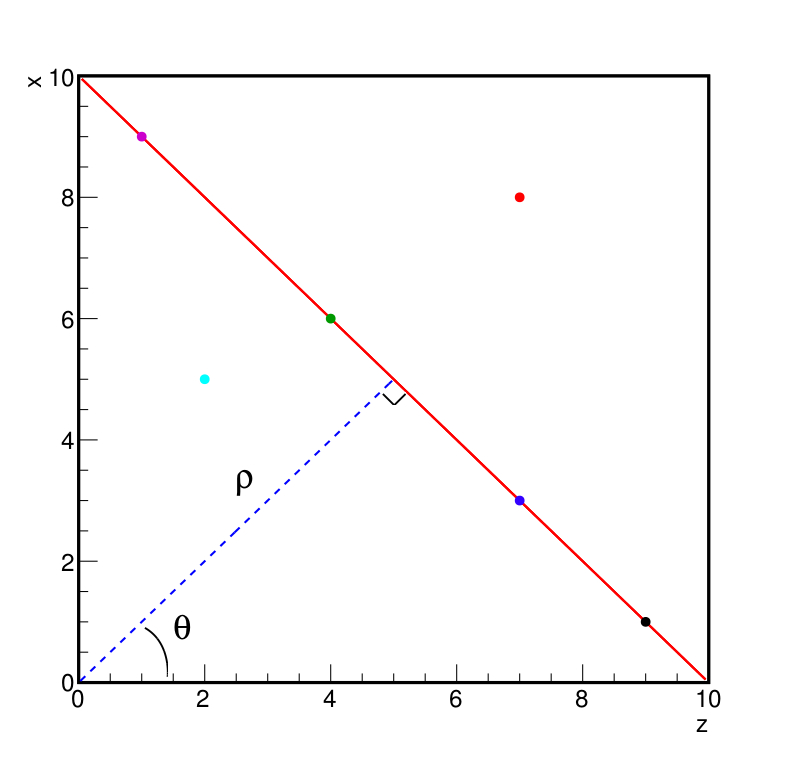
\includegraphics[width=.5\textwidth]{Shower/figs/HTexample.jpg}
  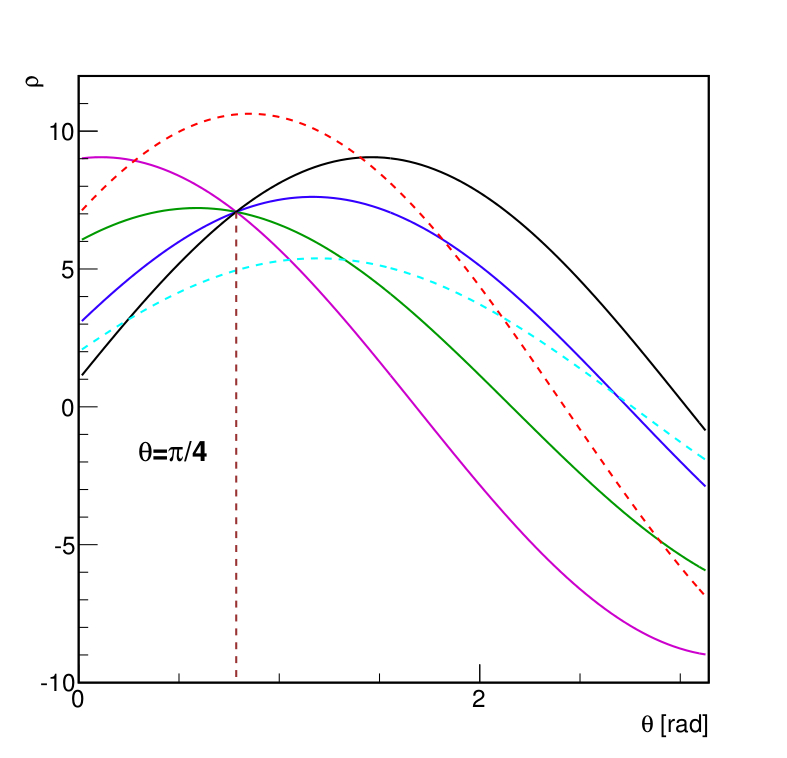
\includegraphics[width=.5\textwidth]{Shower/figs/HTspace.jpg}
  \caption{Illustration de la méthode de Transformée de Hough. Pour chaque points de la figure de gauche, une courbe est associée sur la figure de droite avec la même couleur. Les courbes associées aux points de la droite s'intersectent en un seul point dans le plan~($\theta$,$\rho$).}
  \label{fig.ht_example}
\end{figure}
La méthode de Transformée de Hough est relativement simple à mettre en œuvre pour détecter des lignes droites. Des variantes, plus compliquées, permettent d'identifier des formes plus complexes comme des arcs de cercle. Ces variantes restent basées sur le même principe. Pour trouver des points localisés sur une ligne droite dans un plan (exemple $(xOz)$), les coordonnées de ces points sont transformées en courbes dans le plan polaire~($\theta$,$\rho$)~\cite{houghDuda}:
\begin{equation}
  \label{eq.hough}
  \rho=zcos\theta + xsin\theta
\end{equation} 
Dans le plan polaire~($\theta$,$\rho$), les courbes associées à des points alignés dans le plan $(xOz)$ s'intersectent en un seul point de coordonnée $(\theta_0,\rho_0)$. Ce principe est illustré par la figure~\ref{fig.ht_example}. Ainsi, la recherche de lignes droites revient à trouver des nœuds dans le plan polaire. Le nombre de courbes se croisant en un nœud sera un paramètre essentiel pour reconstruire les traces dans les gerbes hadroniques.

Cependant, la méthode que nous venons de décrire ne peut pas être appliquée directement aux données du SDHCAL. Il faut en effet tenir compte de la résolution spatiale du détecteur. Le plan~($\theta$,$\rho$) doit donc être discrétisé et transformé en un histogramme 2D. Un nœud est alors remplacé par une classe de l’histogramme et le nombre de courbes se croisant dans le nœud correspond au nombre d'entrées dans cette classe.

\subsection{Transformée de Hough dans le SDHCAL}
Dans les cœurs des gerbes hadroniques et électromagnétiques, de nombreux points sont alignés alors que la motivation de la méthode est d'identifier les traces générées par une seule particule. Il faut donc une procédure pour filtrer la partie dense des cascades avant d'appliquer la méthode. De plus, la Transformée de Hough est appliquée aux amas reconstruits plutôt qu'aux cellules touchées. Ceci permet d'absorber le phénomène de multiplicité et de gagner du temps de calcul. Les amas de hits sont construits avec la méthode standard (cf. chapitre~\ref{chap.sdhcal}). Les coordonnées des barycentres des amas sont utilisées comme variables de position par la suite. Un amas appartient à la partie dense de la cascade si son nombre de hits est strictement supérieur à 4; si le nombre d'amas situés à moins de 5 cm de celui-ci est supérieur à 2; ou si un amas avec plus de 4 cellules touchées est trouvé dans un rayon de moins de 5 cm. Les amas de la partie dense ne sont pas utilisés dans l'algorithme de reconstruction des traces. La Transformée de Hough est ensuite appliquée aux amas restants:
\begin {enumerate}[~~1-]
\begin{figure}[!ht]
  \subfigure[]{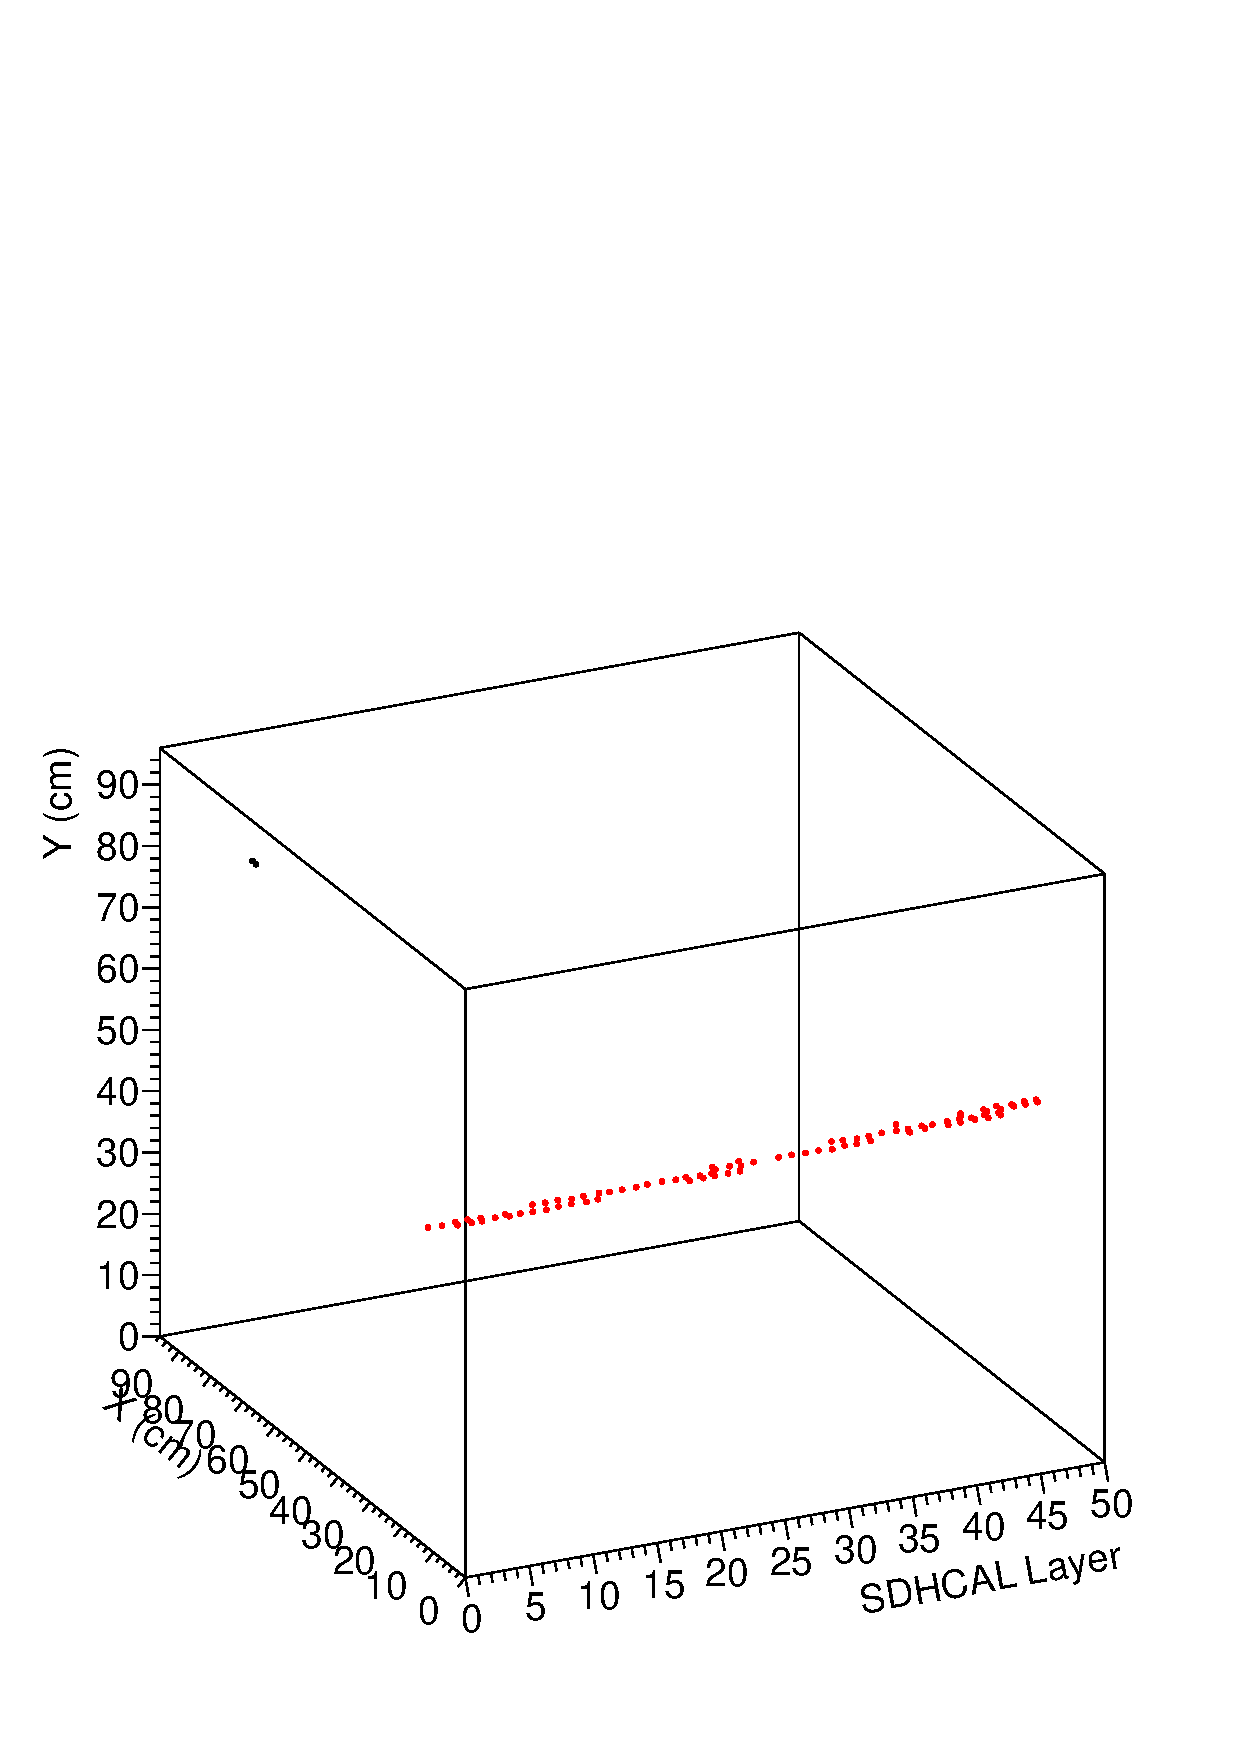
\includegraphics[width=.5\textwidth]{Shower/figs/muon-50-data.pdf}}
  \subfigure[]{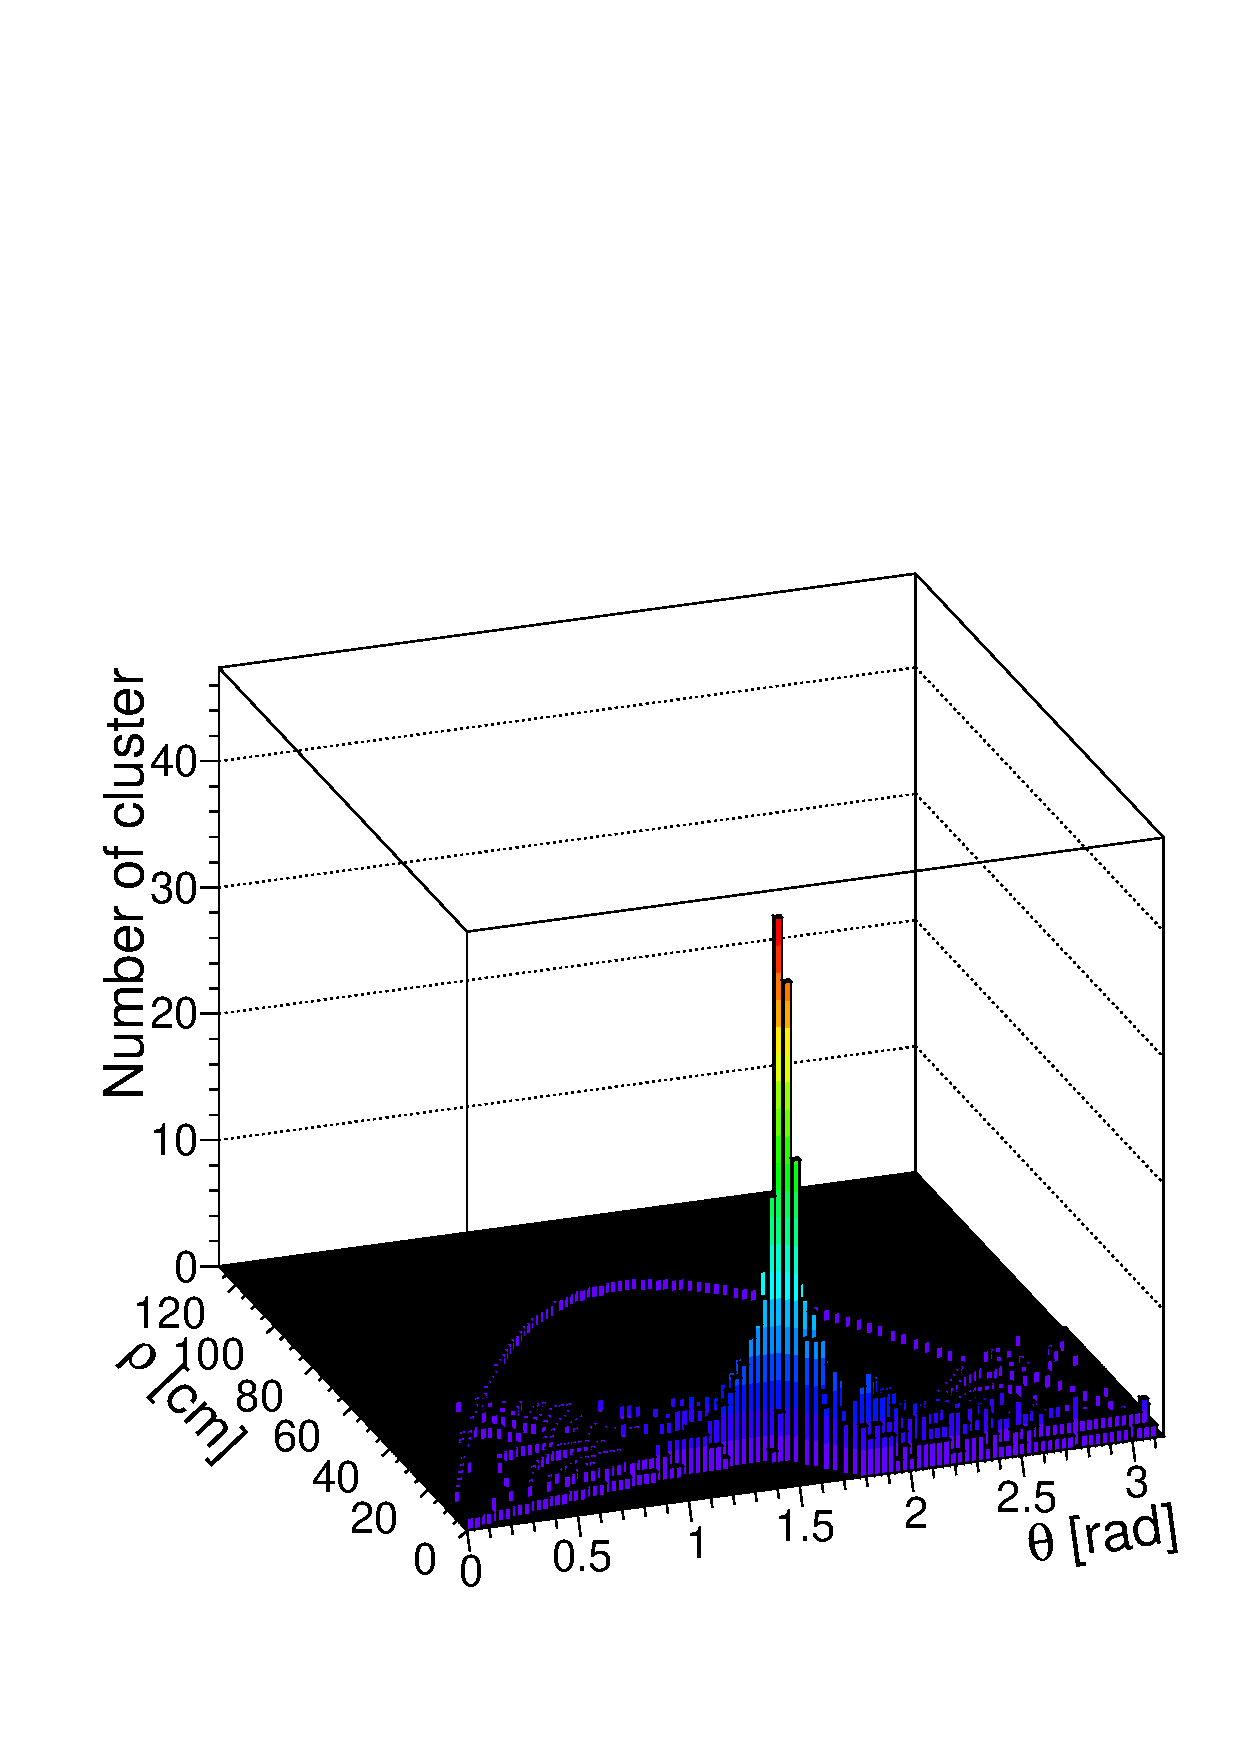
\includegraphics[width=.5\textwidth]{Shower/figs/muon-50-HS_2.pdf}}
  \caption{(a): Image de la trace laissée par un muon dans le SDHCAL. Les points en rouge correspondent aux hits appartenant à la trace reconstruite par la méthode de Transformée de Hough. (b): Histogramme 2D associé correspondant à la transformation du plan $(xOz)$. La courbe associée aux deux hits de bruits, points en noir sur la figure (a), ne croisent pas les autres courbent au maximum de l'histogramme, sur la figure (b).}
  \label{fig.ht_muon}
\end{figure}
\item Pour chacun de ces amas et pour 100 valeurs uniformément espacées de $\theta_x$ dans l'intervalle $[\frac{-\pi}{2},\frac{\pi}{2}]$, la distance $\rho_x$ est calculée avec la transformation donnée par l'équation~\ref{eq.hough} (avec le plan $(xOz)$). Les valeurs de $\rho_x$ sont arrondies à l'entier le plus proche. Pour chaque couple ${(\theta_x,\rho_x)}_i$ ainsi obtenu, un compteur dédié $C_{x,i}$ est incrémenté d'une unité. La figure~\ref{fig.ht_muon}(a) montre un événement muon, enregistré sur la ligne H6 du SPS, dans le prototype SDHCAL. La figure~\ref{fig.ht_muon}(b) est l’histogramme 2D correspondant à la transformation dans le plan $(xOz)$. Cet histogramme montre le nombre d'entrées pour tous les couples ${(\theta_x ,\rho_x)}_i$ obtenus avec la transformation. 
\item \label{step.hg2} Le maximum $C_{x,max}$ des $C_{x,i}$ est déterminé et les amas correspondant sont sélectionnés seulement si $C_{x,max}\geq 6$. L'algorithme s'arrête si $C_{x,max}<6$.
\item La même procédure est appliquée dans le plan $(yOz)$ uniquement avec les amas sélectionnés: les distances $\rho_y$ sont calculées pour 100 valeurs de $\theta_y$ dans l'intervalle $[\frac{-\pi}{2},\frac{\pi}{2}]$ et un compteur $C_{y,i}$ est incrémenté chaque fois que le couple ${(\theta_y,\rho_y)}_i$ est trouvé. 
\item Si le maximum $C_{y,max}$ est supérieur à 6, une trace est créée. Certains amas de cellules touchées peuvent être alignés avec la trace sans pour autant être générés par la même particule. Ainsi, pour chaque amas de la trace, si aucun autre amas de la trace n'est trouvé à moins de trois plans, cet amas est rejeté de la trace. 
\item Une régression linéaire permet de déterminer l'équation de la droite. La trace est conservée uniquement si le $\chi^2$ obtenu avec la régression linéaire est inférieur à 100. Des amas de hits peuvent ensuite être ajoutés à la trace lorsqu'ils sont proches ($<2~cm$) de la droite. 
\item Une procédure permet de séparer une trace en plusieurs traces si ses fragments sont trop éloignés les uns des autres (plus de trois plans).% En effet, il peut arriver que 
\item Les compteurs $C_{x,i}$ sont décrémentés d'une unité pour chaque amas de hits appartenant à la trace construite et l'algorithme reprend à l'étape~\ref{step.hg2}. Cette étape permet de ne pas reconstruire plusieurs fois la même trace. De plus, cette procédure assure qu'un amas de cellules touchées ne participe qu'à une seule trace au maximum.
\end{enumerate}
\begin{figure}[!ht]
  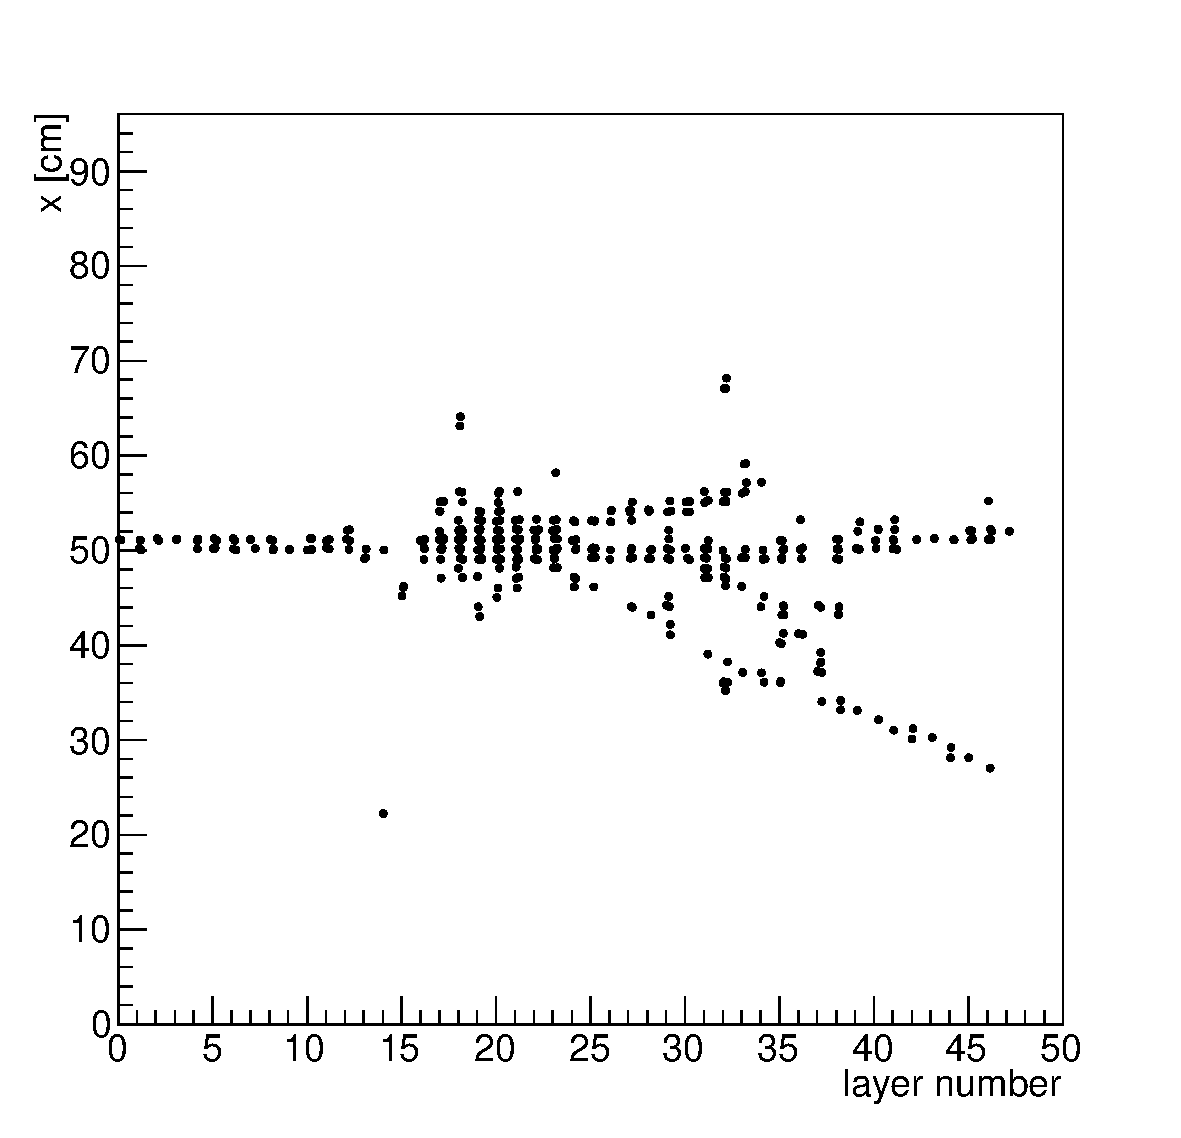
\includegraphics[width=.32\textwidth]{Shower/figs/715747_319_1_X.pdf}
  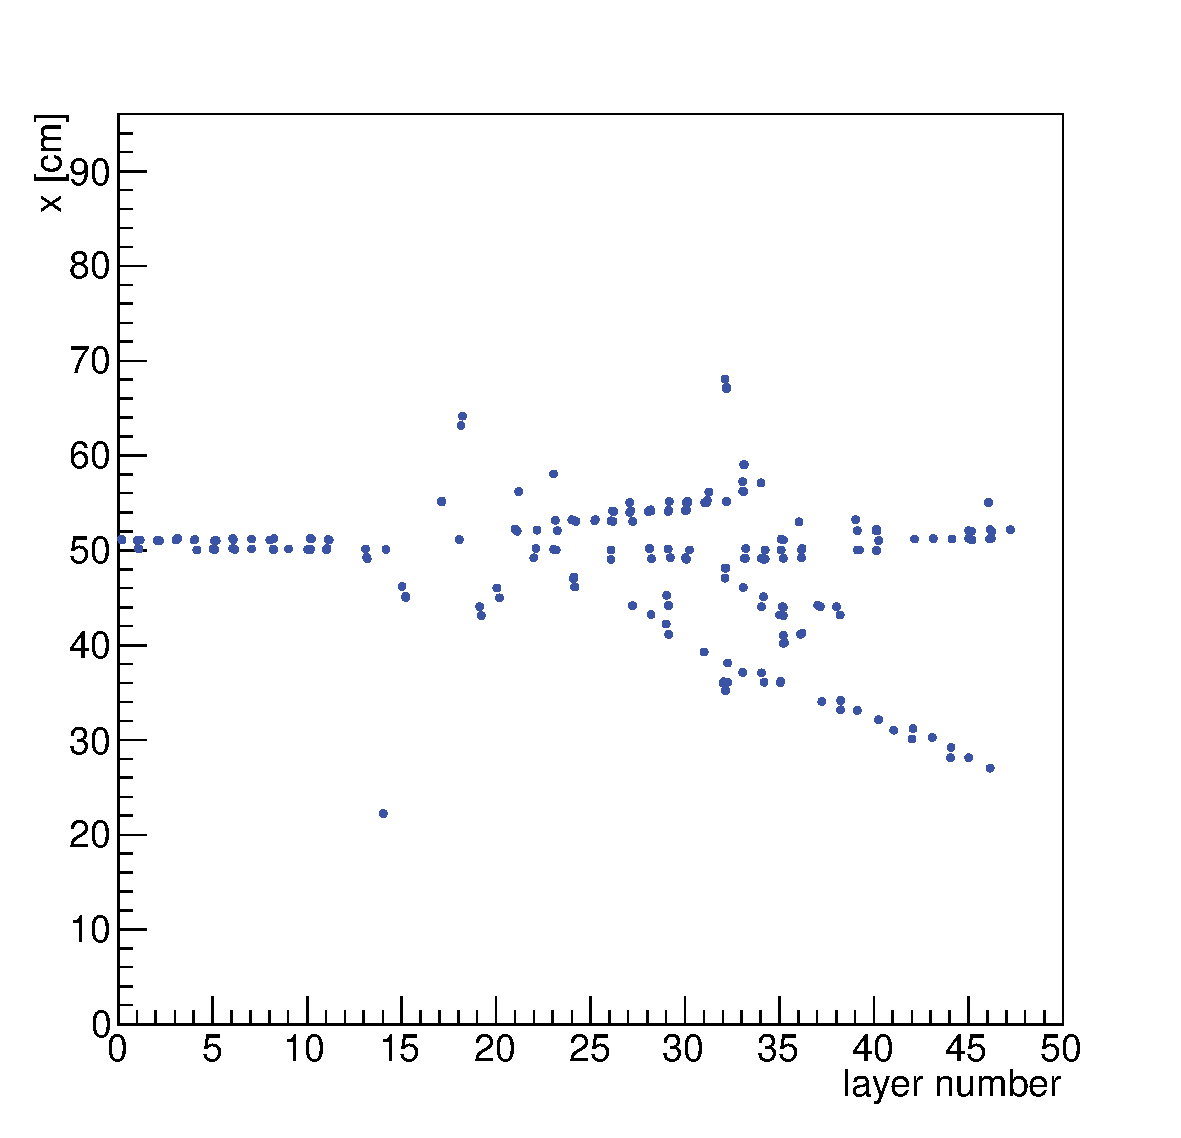
\includegraphics[width=.32\textwidth]{Shower/figs/715747_319_2_X.pdf}
  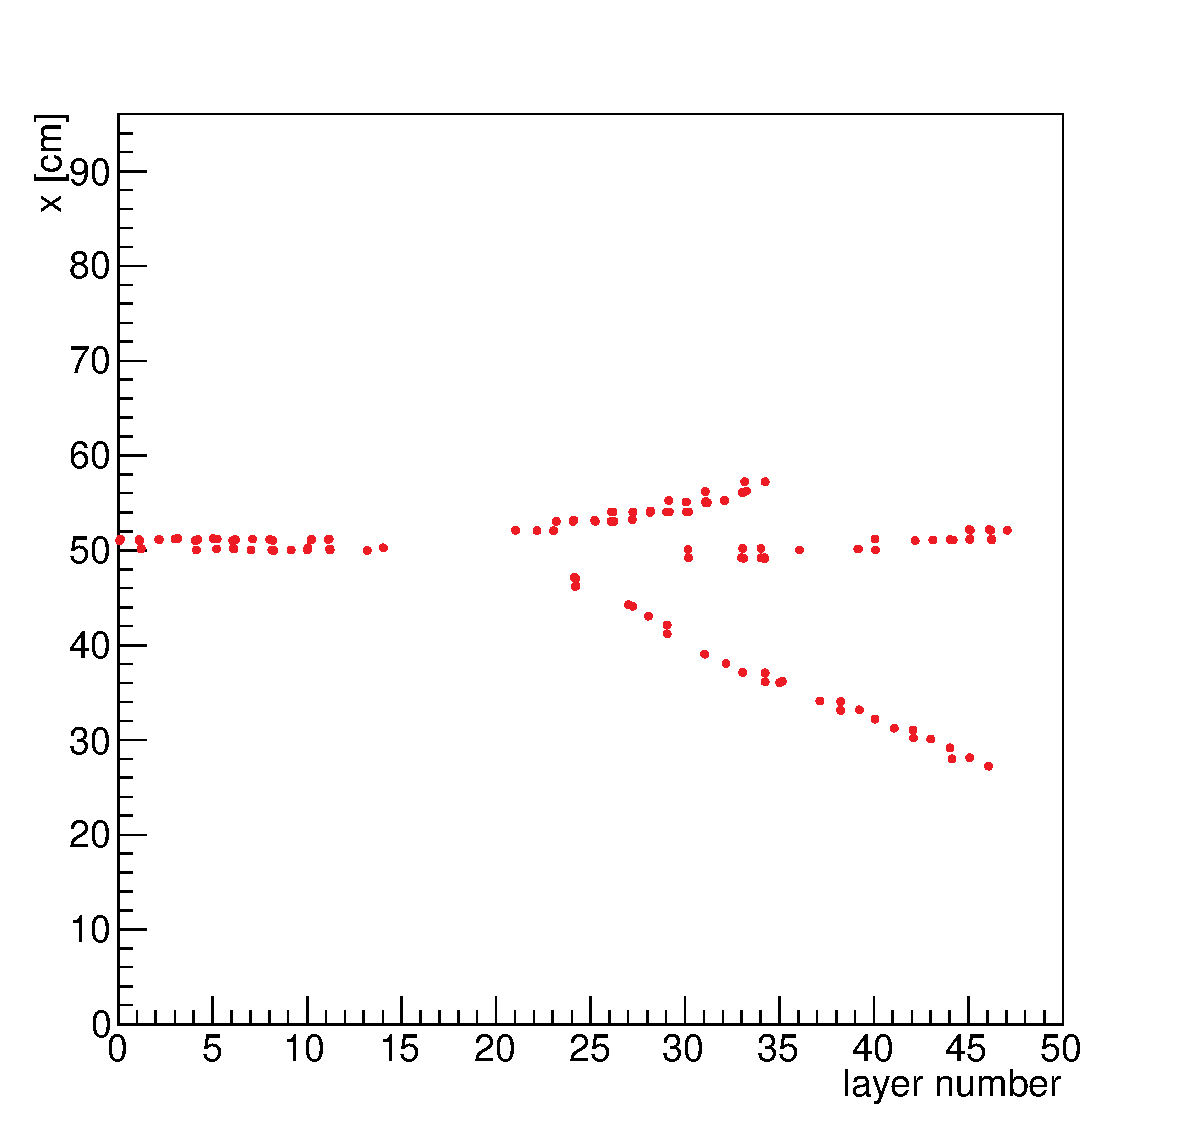
\includegraphics[width=.32\textwidth]{Shower/figs/715747_319_3_X.pdf}
  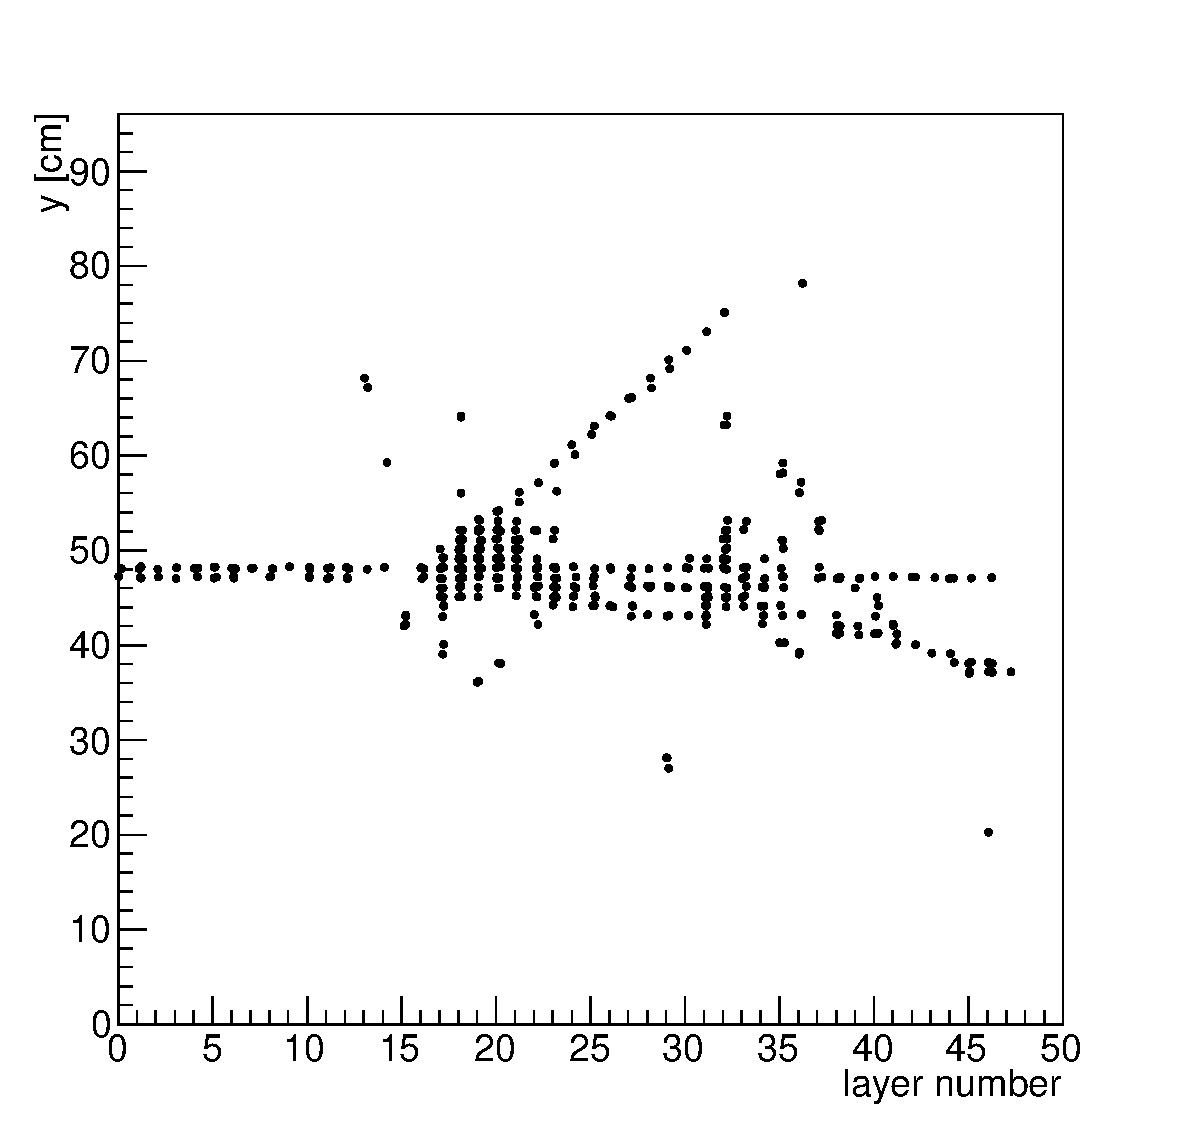
\includegraphics[width=.32\textwidth]{Shower/figs/715747_319_1_Y.pdf}
  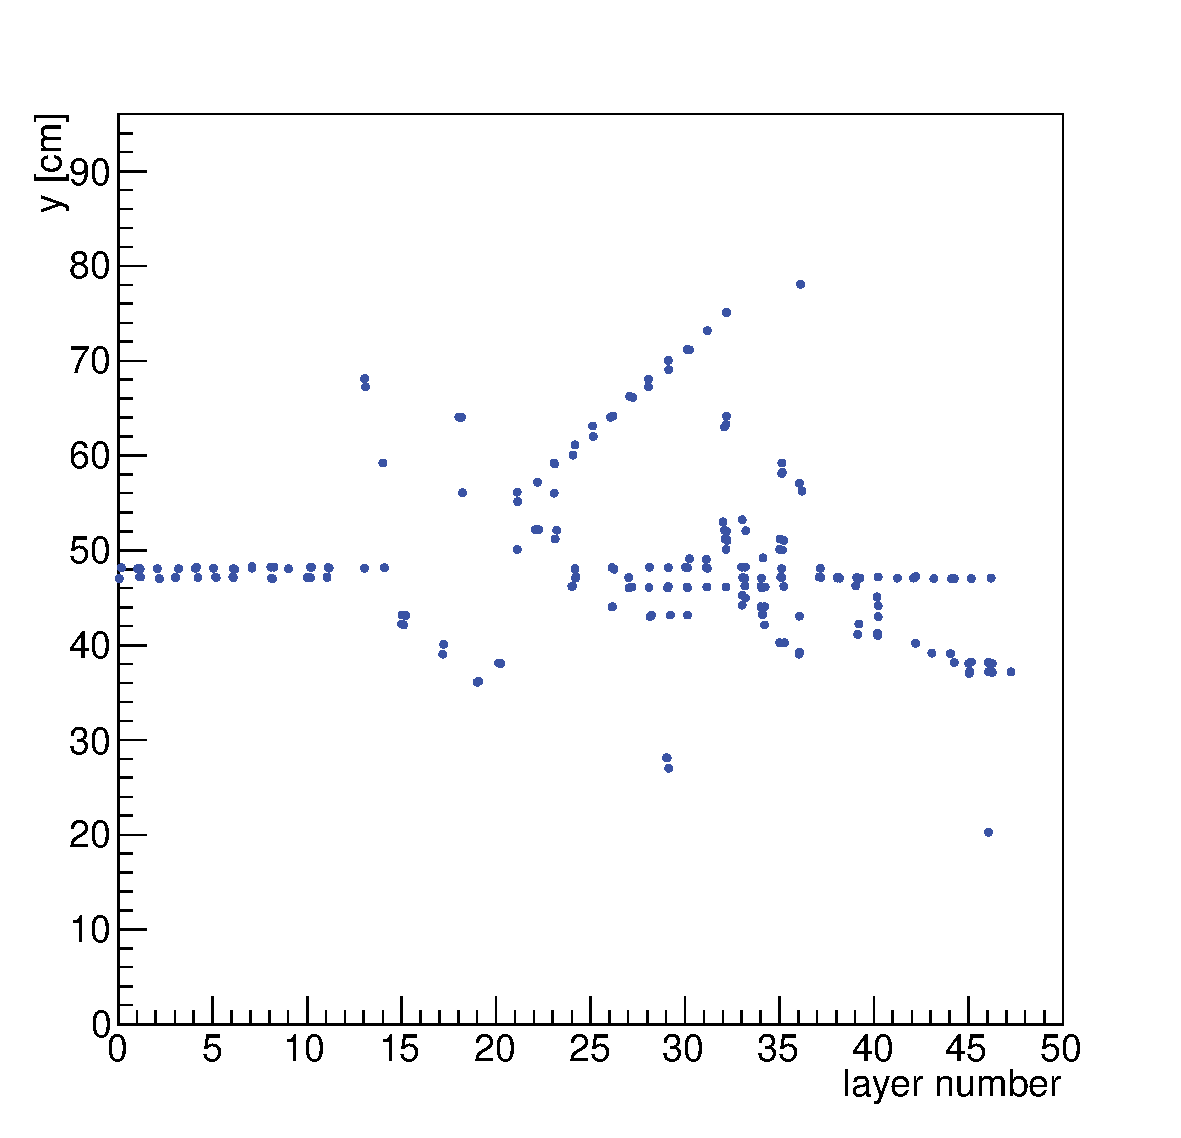
\includegraphics[width=.32\textwidth]{Shower/figs/715747_319_2_Y.pdf}
  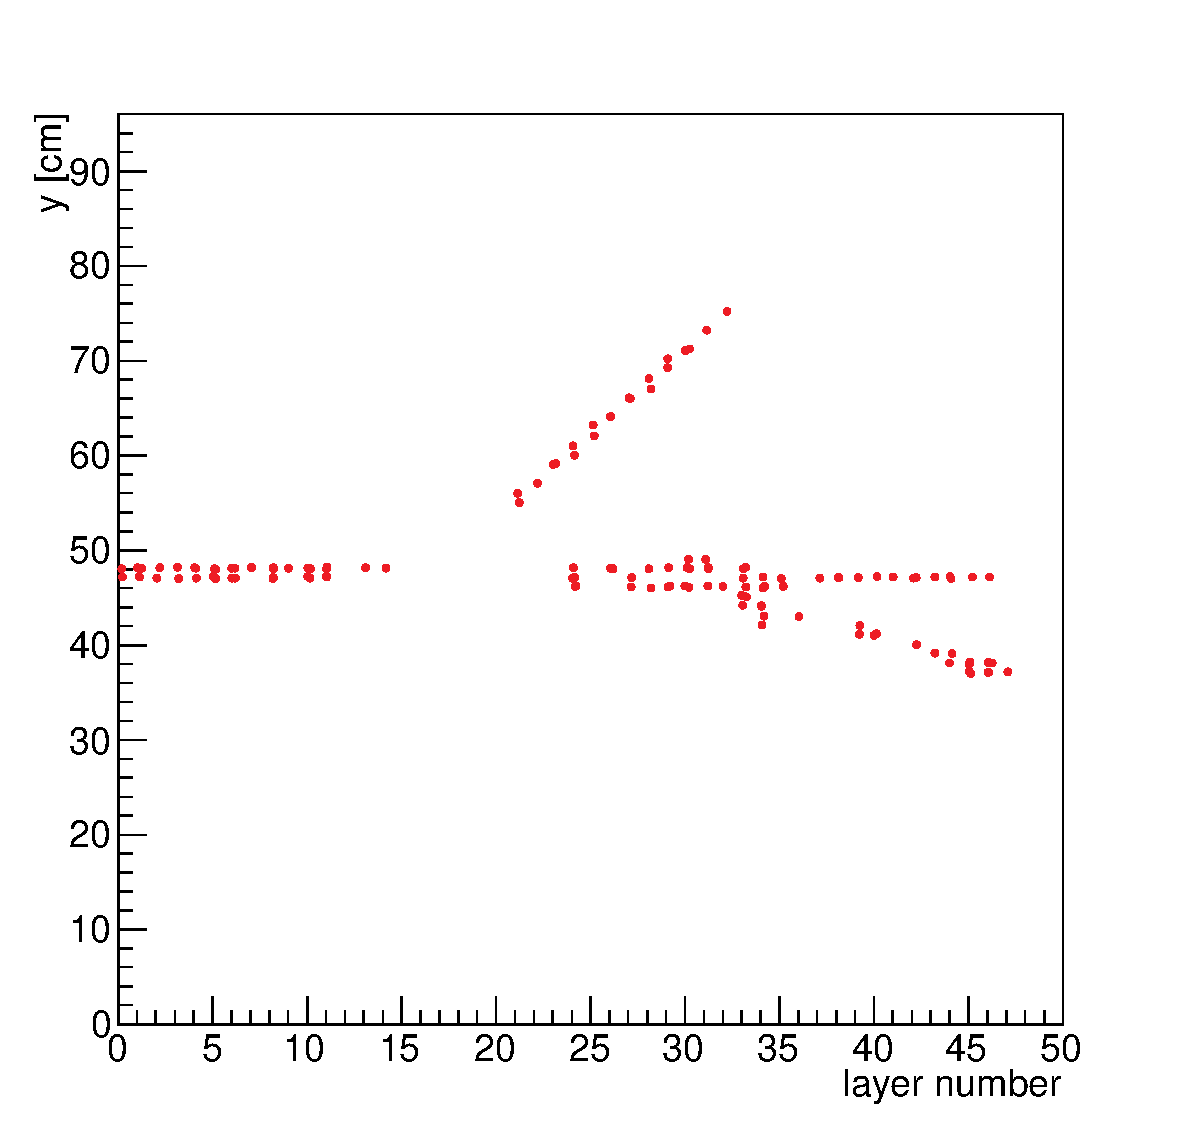
\includegraphics[width=.32\textwidth]{Shower/figs/715747_319_3_Y.pdf}
  \caption{Image d'une gerbe hadronique de 30 $GeV$ dans le SDHCAL dans le plan~$(xOz)$ (en haut) et le plan~$(yOz)$ (en bas) illustrant les différentes étapes de la reconstruction des traces. La colonne de gauche montre tous les hits de l'événement, la colonne du milieu présente les hits appartenant aux amas de la partie non dense et la colonne de droite présente les hits le long des traces reconstruites par la méthode de transformée de Hough.\label{fig.pi-_hough}}
\end{figure}
La figure~\ref{fig.pi-_hough} présente un exemple de gerbe hadronique de 30 $GeV$, enregistré sur la ligne H6 du SPS. La première colonne montre toutes les cellules touchées de l'événement. La deuxième présente les hits appartenant aux groupes de la partie non dense. La troisième colonne indique les hits des traces reconstruites par la méthode de Transformée de Hough. 
\newpage
\subsection{Performance de la Transformée de Hough}
\begin{figure}[!ht]
  \centering
  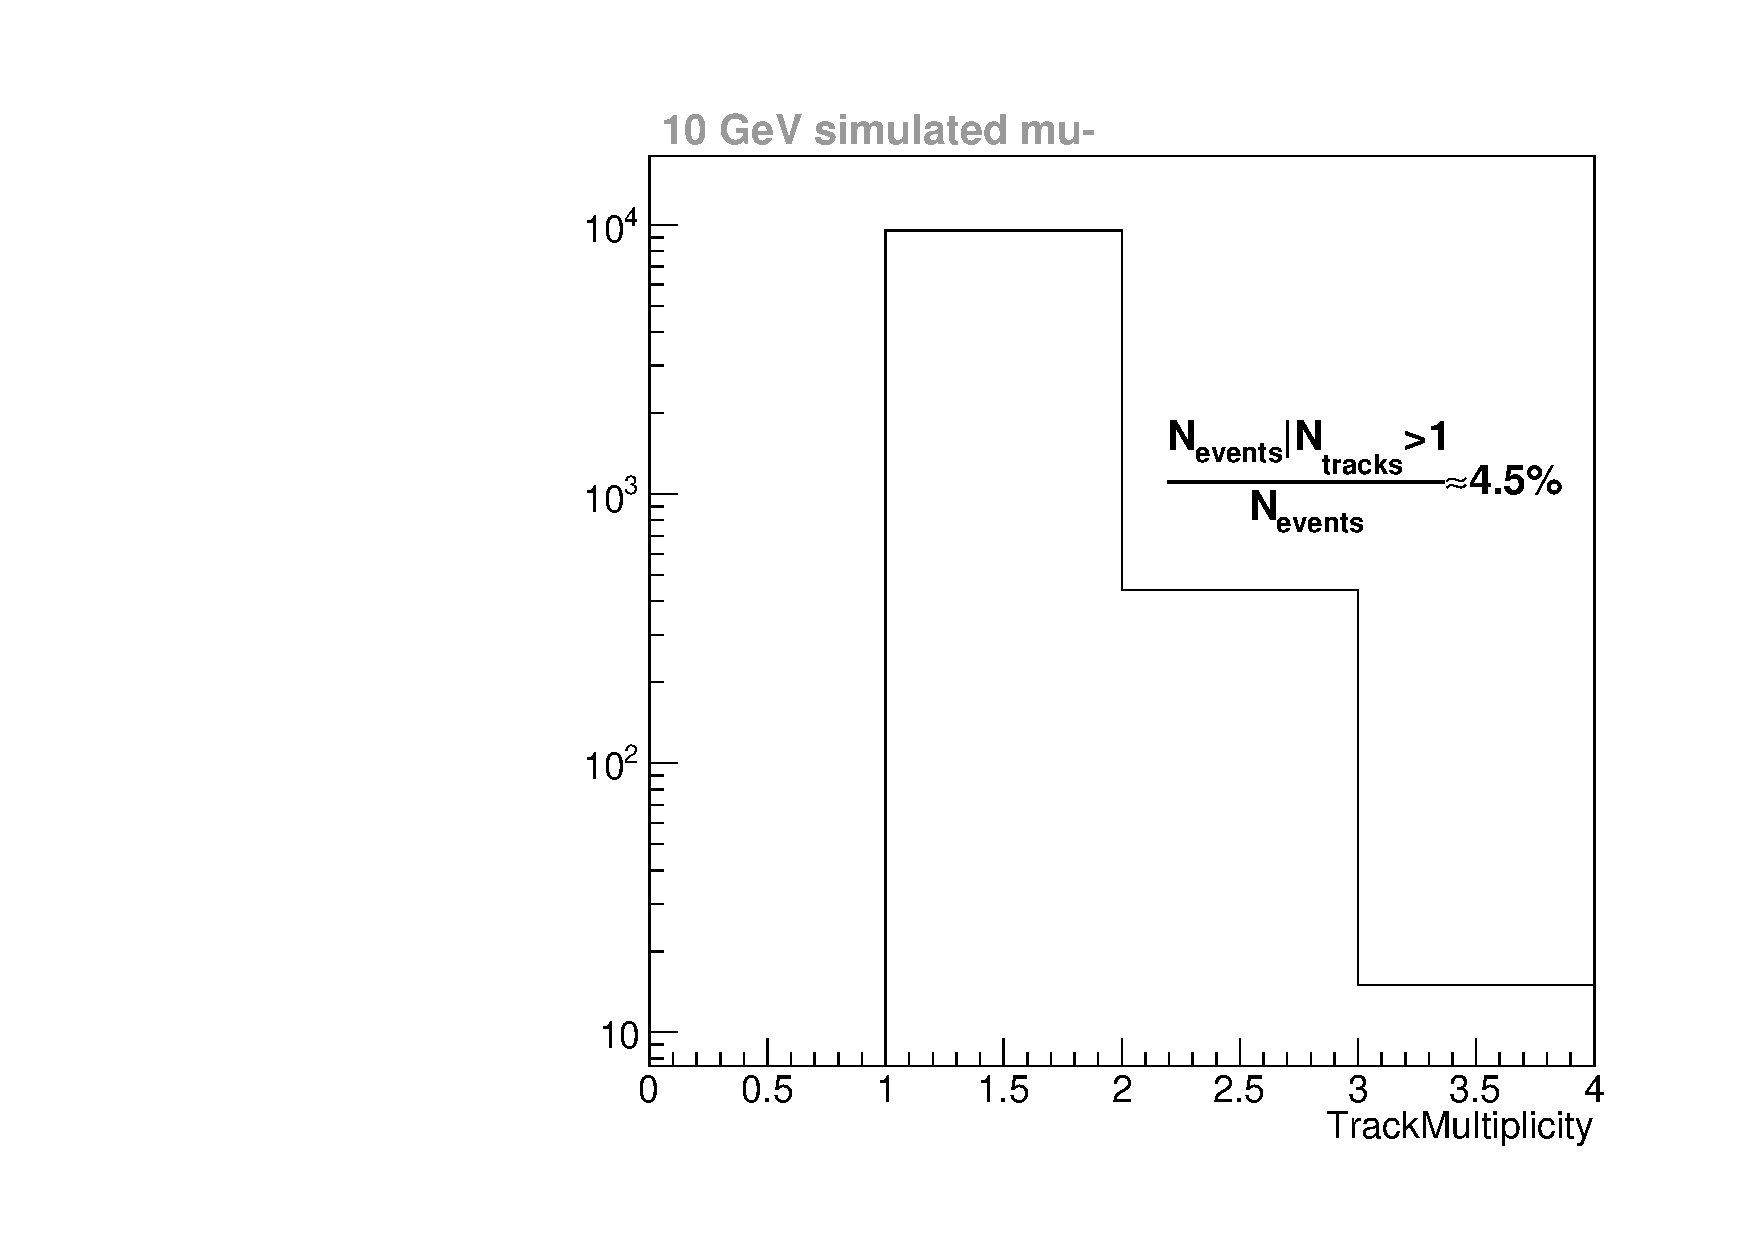
\includegraphics[width=.5\textwidth]{Shower/figs/ntrack_mu-_10GeV_ftfp_bert_hp.pdf}
  \caption{Distribution du nombre de traces reconstruites par la méthode de Transformée de Hough pour une simulation de muons à 10 $GeV$.\label{fig.ntrack_mu-_sim}}
\end{figure}
La performance de la méthode de Transformée de Hough est étudiée avec les muons. La figure~\ref{fig.ntrack_mu-_sim} montre le nombre de traces reconstruites par la méthode pour un échantillon de muons à 10 $GeV$ simulé dans le SDHCAL. Les muons radiatifs sont préalablement filtrés (cf. section~\ref{sec.pi_selection} du chapitre~\ref{chap.sdhcal}). La méthode reconstruit toujours au moins une trace et le nombre d'événements avec deux traces reconstruites ou plus est faible ($\approx 4.5\%$). La méthode est aussi testée avec les données expérimentales. Les événements sont identifiés comme des muons s'ils satisfont les mêmes conditions que celles décrites dans la section~\ref{sec.muons} du chapitre~\ref{chap.sdhcal}.

\begin{figure}[!ht]
  \centering
  \subfigure[]{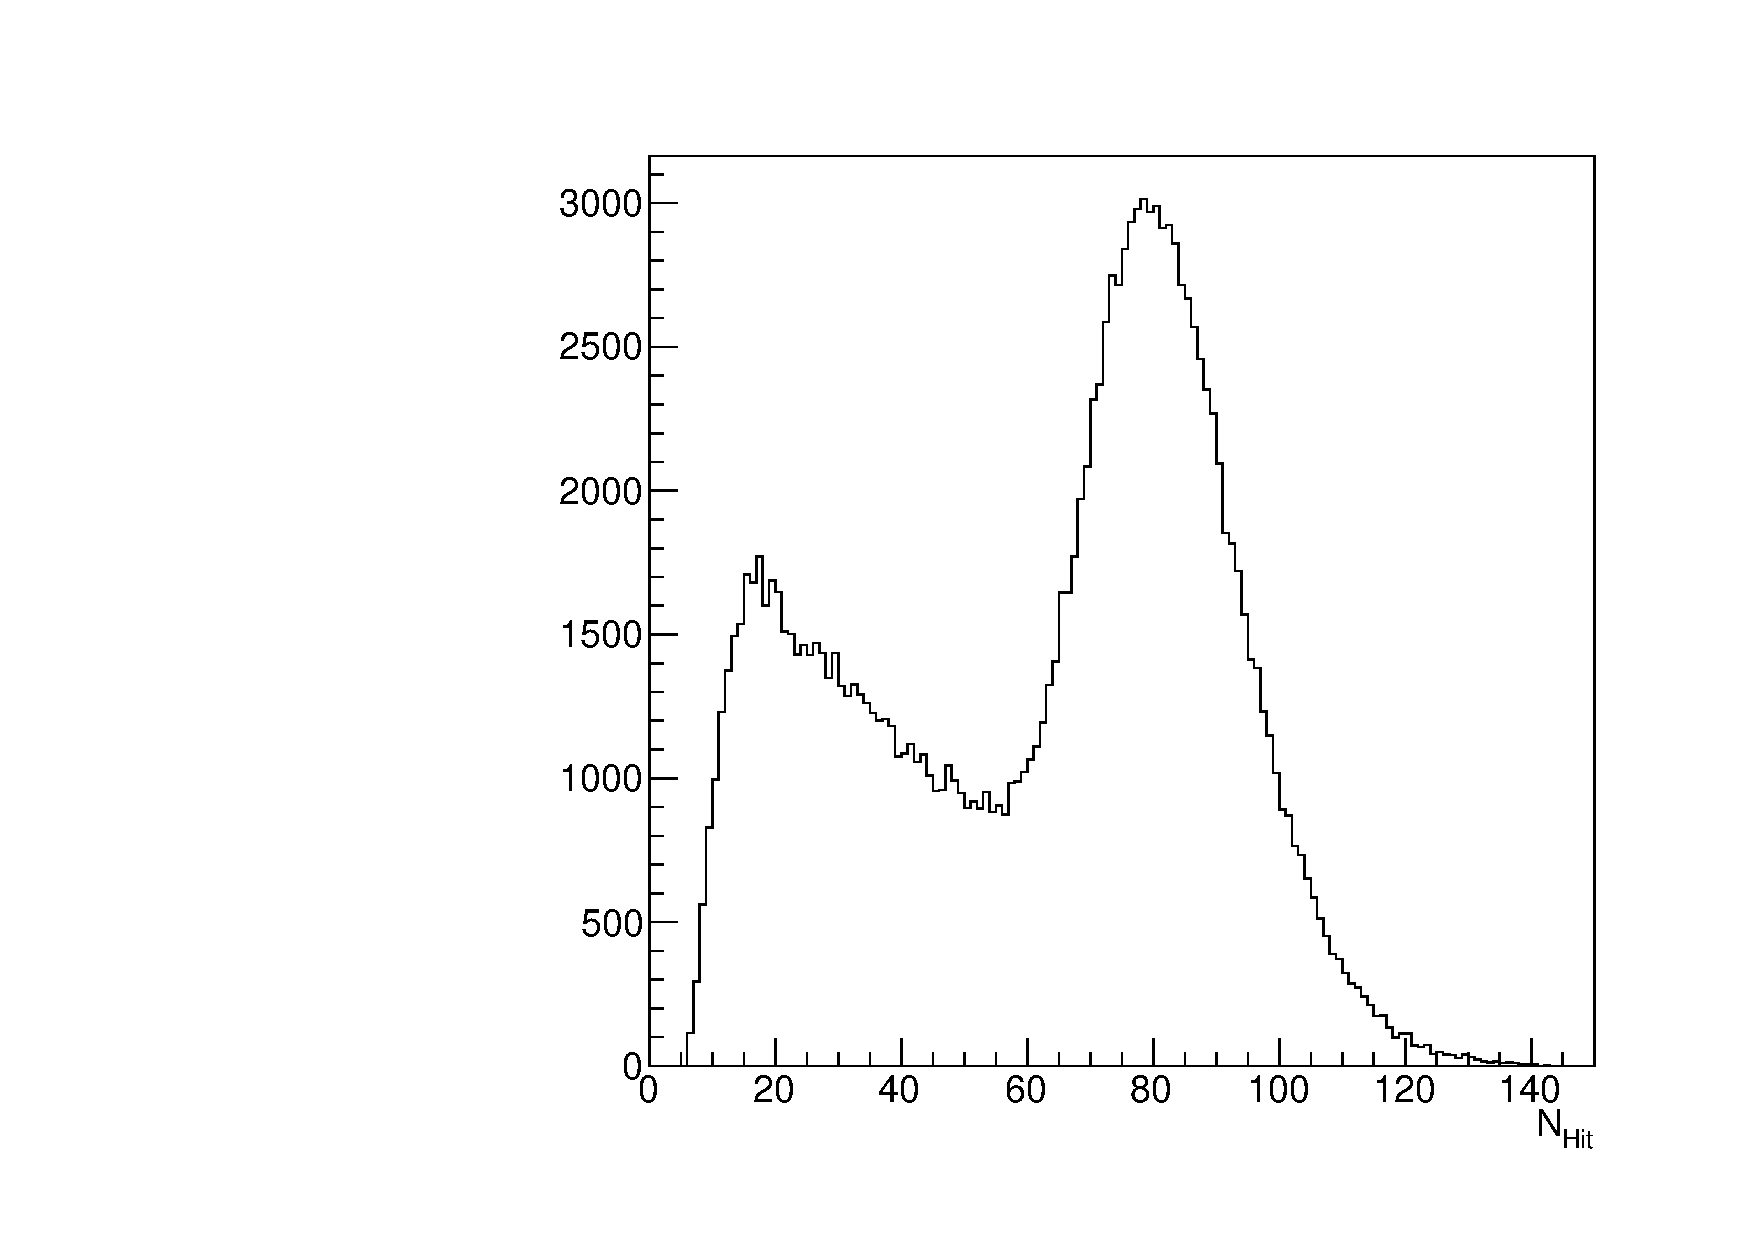
\includegraphics[width=.45\textwidth]{Shower/figs/nhit_mu-_715747.pdf}}
  \subfigure[]{\includegraphics[width=.45\textwidth]{Shower/figs/ntrack_mu-_715747.pdf}}
  \caption{(a): Distribution du nombre de cellules touchées après la sélection des muons. (b): Distribution du nombre de traces reconstruites pour les muons sélectionnés.\label{fig.ntrack_mu-_dat}}
\end{figure}
La figure~\ref{fig.ntrack_mu-_dat}(a) montre la distribution du nombre de cellules touchées pour des événements muons. Les deux pics correspondent aux réponses du SDHCAL aux muons cosmiques (autour de 20 hits) et aux muons du faisceau (autour de 85 hits). La figure~\ref{fig.ntrack_mu-_dat}(b) présente le nombre de traces reconstruites par la Transformée de Hough. Le rapport du nombre d'événements pour lesquels la reconstruction d'au moins une trace échoue est de 2.87$\%$. Ce rapport tombe à 1.15$\%$ lorsque l'angle entre la trajectoire de la particule et l'axe $Oz$ est inférieur à 45°. Cette coupure rejette les événements issus des particules cosmiques. Le nombre de plans touchés par les particules cosmiques est plus faible que pour les muons du faisceau. 
%De plus, nous avons vu que la multiplicité augmente sensiblement avec l'angle d'incidence (cf. figure~\ref{fig.mul_vs_theta} du chapitre~\ref{chap.simulation}). Ainsi, certains groupes de coups des événements cosmiques sont identifiés comme appartenant à la partie dense d'une gerbe hadronique. Ces facteurs expliquent l'échec de la méthode à reconstruire les traces de certains événements.

L'étude des muons avec la simulation et les données indique tout de même une bonne efficacité de la méthode de Transformée de Hough pour reconstruire des traces. Cette méthode a aussi été testée sur les gerbes électromagnétiques pour vérifier que cette méthode ne reconstruit pas de traces accidentellement. La figure~\ref{fig.e-_ntrack} montre la distribution du nombre de traces reconstruites à 20 et 50 $GeV$ pour les données et la simulation. Pour une grande majorité de gerbes électromagnétiques, le nombre de traces reconstruites est nulle. Le rapport du nombre d'événements avec au moins une trace et le nombre total d'événements varie entre 1$\%$ à 10 $GeV$ et 2$\%$ à 50 $GeV$ pour les données. Ce rapport est très légèrement inférieur pour la simulation.
\begin{figure}[!ht]
  \centering
  \includegraphics[width=.45\textwidth]{Shower/figs/ntrack_electron_20GeV_AugSep2012.pdf}
  \includegraphics[width=.45\textwidth]{Shower/figs/ntrack_electron_50GeV_AugSep2012.pdf}
  \caption{Distribution du nombre de traces reconstruites pour des gerbes électromagnétiques à 20 et 50 $GeV$. Les données sont représentées par des cercles noirs et la simulation (FTFP\_BERT\_HP) par les histogrammes rouges. \label{fig.e-_ntrack}}
\end{figure}

\subsection{Étude des modèles de simulation des gerbes hadroniques}
La reconstruction des traces dans les gerbes hadroniques est un atout supplémentaire pour discriminer les modèles de simulation. Nous allons étudier trois variables relatives aux traces dans les gerbes hadroniques: le nombre de traces reconstruites, leur longueur, puis leur angle d'émission par rapport à l'axe de la cascade.
\subsubsection{Nombre de traces reconstruites}
\begin{figure}[!ht]
  \centering
  \includegraphics[width=.32\textwidth]{Shower/figs/ntrack_pi-_10GeV_ftfp_bert_hp.pdf}
  \includegraphics[width=.32\textwidth]{Shower/figs/ntrack_pi-_10GeV_qgsp_bert_hp.pdf}
  \includegraphics[width=.32\textwidth]{Shower/figs/ntrack_pi-_10GeV_ftf_bic.pdf}\\
  \includegraphics[width=.32\textwidth]{Shower/figs/ntrack_pi-_30GeV_ftfp_bert_hp.pdf}
  \includegraphics[width=.32\textwidth]{Shower/figs/ntrack_pi-_30GeV_qgsp_bert_hp.pdf}
  \includegraphics[width=.32\textwidth]{Shower/figs/ntrack_pi-_30GeV_ftf_bic.pdf}\\
  \includegraphics[width=.32\textwidth]{Shower/figs/ntrack_pi-_80GeV_ftfp_bert_hp.pdf}
  \includegraphics[width=.32\textwidth]{Shower/figs/ntrack_pi-_80GeV_qgsp_bert_hp.pdf}
  \includegraphics[width=.32\textwidth]{Shower/figs/ntrack_pi-_80GeV_ftf_bic.pdf}
  \caption{Distribution du nombre de traces reconstruites pour les données (ligne H2) et la simulation à 10 (en haut), 30 (au milieu) et 80 $GeV$ (en bas). Les données sont représentées par des cercles noirs et la simulation par les histogrammes pleins. \label{fig.pi-_ntrack}}
\end{figure}
Dans cette étude, la procédure de sélection des gerbes hadroniques ne tient pas compte du critère sur le nombre de traces reconstruites. La figure~\ref{fig.pi-_ntrack} présente les distributions du nombre de traces reconstruites à 10, 30 et 80 $GeV$ pour les données, et trois modèles de simulation (FTFP\_BERT\_HP, QGSP\_BERT\_HP et FTF\_BIC). Le nombre de traces reconstruites pour ces différentes listes présente un accord raisonnable avec les données.
\begin{figure}[!ht]
  \centering
  \includegraphics[width=.44\textwidth]{Shower/figs/NTRACKPIONHP.pdf}
  \includegraphics[width=.44\textwidth]{Shower/figs/NTRACKPIONNOV.pdf}
  \includegraphics[width=.44\textwidth]{Shower/figs/NTRACK_PION_MODEL.pdf}
  \includegraphics[width=.44\textwidth]{Shower/figs/NTRACK_PION_MODEL_NOV.pdf}
  \caption{Nombre moyen de traces reconstruites gràce à la Transformée de Hough, en fonction de l'énergie, pour les données et plusieurs modèles de simulation. Les déviations relatives sont aussi présentées. La colonne de gauche présente une comparaison entre les données de la ligne H6 et les simulations, la colone de droite entre les données de la ligne H2 et les mêmes simulations. La ligne du haut présente des comparaisons entre les données et avec les listes QGSP\_BERT\_HP et FTFP\_BERT\_HP pour des simulations de pions et de protons. La ligne du bas présente les comparaisons avec d'autres listes physiques pour des simulations de pions. La taille des barres d'erreurs est inférieure à celle des points.}
  \label{fig.ntrack_pi-_ebeam}
\end{figure}
%% \begin{figure}[!ht]
%%   \centering
%%   \includegraphics[width=.44\textwidth]{Shower/figs/NTRACKPROTON_FTFP.pdf}
%%   \includegraphics[width=.44\textwidth]{Shower/figs/NTRACKPROTON_QGSP.pdf}
%%   \caption{Nombre moyen de traces reconstruites avec la Transformée de Hough en fonction de l'énergie pour les données, des simulations de pions et de protons avec les listes FTFP\_BERT\_HP (à gauche) et QGSP\_BERT\_HP (à droite). Les déviations relatives sont aussi présentées.}
%%   \label{fig.ntrack_proton_ebeam}
%% \end{figure}

La figure~\ref{fig.ntrack_pi-_ebeam} montre la valeur moyenne du nombre de traces reconstruites en fonction de l'énergie pour les données (sur les lignes H6 et H2) et plusieurs listes physiques. La déviation relative est aussi présentée. Elle est définie par $\frac{<N_{simu}>-<N_{data}>}{<N_{data}>}$ où $<N_{data}>$ et $<N_{simu}>$ sont respectivement les valeurs moyennes du nombre de traces reconstruites pour les données et la simulation. Cette figure montre la différence entre le nombre de traces reconstruites dans les gerbes hadroniques initiées par des pions et des protons pour les listes FTFP\_BERT\_HP et QGSP\_BERT\_HP. 

Le nombre de traces dans les gerbes hadroniques initiées par les protons est plus grand que pour les cascades initiées par des pions. Les données enregistrées sur la ligne H6, contaminée par des protons, présentent aussi un plus grand nombre de traces reconstruites que dans celles enregistrées sur la ligne H2. Ces résultats peuvent s'expliquer par la fraction électromagnétique plus faible dans les gerbes hadroniques initiées par des protons (cf.~section~\ref{sec.fem} du chapitre~\ref{chap.shower}).

Les comparaisons avec les données de la ligne H2, montrent que les différents modèles de simulation de gerbes hadroniques initiées par des pions, reproduisent raisonnablement bien les données. Pour tous les modèles, la déviation relative est inférieure à 10$\%$ sur toute la gamme d'énergie. Enfin, notons que la liste FTFP\_BERT(\_HP) est celle qui reproduit le mieux les données, avec jusqu'à 5-6$\%$ de traces reconstruites en plus des autres modèles de simulation. 
%La liste QGSP\_BIC produit entre 10 et 25$\%$ moins de traces que les données. 
%Les autres listes physiques présentent un assez bon accord avec les données. , est inférieure à 10$\%$ sur toute la gamme d'énergie pour ces listes. Cependant, Le nombre de traces est légèrement surestimé par la liste FTFP\_BERT(\_HP). Le nombre de traces est aussi étudié avec des simulation de gerbes hadroniques induites par des protons. 

\subsubsection{Longueur des traces reconstruites}
La longueur des traces est mesurée en unité de longueur d'interaction $\lambda_I^\pi$ et correspond à la distance entre le barycentre du premier amas de hits et le barycentre du dernier amas. Pour obtenir une longueur en unité de longueur d'interaction, est prise en compte uniquement l'épaisseur traversée dans les plaques d'absorbeur en acier. La figure~\ref{fig.pi-_tracklength} présente les distributions des longueurs des traces reconstruites à 10, 30 et 80 $GeV$ pour les données et plusieurs modèles de simulation (FTFP\_BERT\_HP, QGSP\_BERT\_HP et FTF\_BIC). 
\begin{figure}[!ht]
  \includegraphics[width=.32\textwidth]{Shower/figs/tracklength_pi-_10GeV_ftfp_bert_hp.pdf}
  \includegraphics[width=.32\textwidth]{Shower/figs/tracklength_pi-_10GeV_qgsp_bert_hp.pdf}
  \includegraphics[width=.32\textwidth]{Shower/figs/tracklength_pi-_10GeV_ftf_bic.pdf}\\
  \includegraphics[width=.32\textwidth]{Shower/figs/tracklength_pi-_30GeV_ftfp_bert_hp.pdf}
  \includegraphics[width=.32\textwidth]{Shower/figs/tracklength_pi-_30GeV_qgsp_bert_hp.pdf}
  \includegraphics[width=.32\textwidth]{Shower/figs/tracklength_pi-_30GeV_ftf_bic.pdf}\\
  \includegraphics[width=.32\textwidth]{Shower/figs/tracklength_pi-_80GeV_ftfp_bert_hp.pdf}
  \includegraphics[width=.32\textwidth]{Shower/figs/tracklength_pi-_80GeV_qgsp_bert_hp.pdf}
  \includegraphics[width=.32\textwidth]{Shower/figs/tracklength_pi-_80GeV_ftf_bic.pdf}
  \caption{Distribution de la longueur des traces reconstruites pour les données (ligne H2) et la simulation à 10 (en haut), 30 (au milieu) et 80 $GeV$ (en bas). Les données sont représentées par des cercles noirs et la simulation par les histogrammes pleins. \label{fig.pi-_tracklength}}
\end{figure}
\begin{figure}[!ht]
  \centering
  \includegraphics[width=.44\textwidth]{Shower/figs/TRACKLENGTHPIONHP.pdf}
  \includegraphics[width=.44\textwidth]{Shower/figs/TRACKLENGTHPIONNOV.pdf}
  \includegraphics[width=.44\textwidth]{Shower/figs/TRACKLENGTH_PION_MODEL.pdf}
  \includegraphics[width=.44\textwidth]{Shower/figs/TRACKLENGTH_PION_MODEL_NOV.pdf}
  \caption{Moyenne des longueurs des traces reconstruites gràce à la Transformée de Hough en fonction de l'énergie pour les données et plusieurs modèles de simulation. Les déviations relatives sont aussi présentées. La colonne de gauche présente une comparaison entre les données de la ligne H6 et les simulations, la colone de droite entre les données de la ligne H2 et les mêmes simulations. La ligne du haut présente des comparaisons entre les données et avec les listes QGSP\_BERT\_HP et FTFP\_BERT\_HP pour des simulations de pions et de protons. La ligne du bas présente les comparaisons avec d'autres listes physiques pour des simulations de pions.}
  \label{fig.tracklength_pi-_ebeam}
\end{figure}

La figure~\ref{fig.tracklength_pi-_ebeam} montre la valeur moyenne des longueurs des traces reconstruites en fonction de l'énergie pour les données (ligne H6 et H2) et plusieurs listes physiques. L'accord entre les données et les différents modèles de simulation est très satisfaisant. La déviation relative, définie par $\frac{<L_{simu}>-<L_{data}>}{<L_{data}>}$ (avec $<L_{simu}>$ et $<L_{data}>$ les longueurs moyennes des traces dans la simulation et les données respectivement), est inférieure à 5$\%$ sur toute la gamme d'énergie pour toutes les listes physiques. La longueur des traces dans les gerbes hadroniques est principalement conditionnée par la longueur d'interaction et la perte d'énergie des particules chargées par ionisation. Ces grandeurs sont maintenant bien connues pour beaucoup de matériaux et il n'est donc pas étonnant de trouver un bon accord entre la simulation et les données sur les longueurs des traces. 
La figure~\ref{fig.tracklength_pi-_ebeam} montre de très légères différences pour la longueur des traces reconstruites entre les gerbes hadroniques initiées par des pions et celles initiées par des protons. La longueur des traces dans les cascades initiées par des protons est en moyenne 3$\%$ plus faible que pour les pions. La rapport des longueurs d’interaction entre les protons et les pions ($\lambda_{pi}/\lambda_{p}=1.22$) permet d'expliquer les différences de longueur des traces reconstruites. 

\subsubsection{Angle d'émission des traces reconstruites}
\begin{figure}[!ht]
  \includegraphics[width=.32\textwidth]{Shower/figs/trackangle_pi-_10GeV_ftfp_bert_hp.pdf}
  \includegraphics[width=.32\textwidth]{Shower/figs/trackangle_pi-_10GeV_qgsp_bert_hp.pdf}
  \includegraphics[width=.32\textwidth]{Shower/figs/trackangle_pi-_10GeV_ftf_bic.pdf}\\
  \includegraphics[width=.32\textwidth]{Shower/figs/trackangle_pi-_30GeV_ftfp_bert_hp.pdf}
  \includegraphics[width=.32\textwidth]{Shower/figs/trackangle_pi-_30GeV_qgsp_bert_hp.pdf}
  \includegraphics[width=.32\textwidth]{Shower/figs/trackangle_pi-_30GeV_ftf_bic.pdf}\\
  \includegraphics[width=.32\textwidth]{Shower/figs/trackangle_pi-_80GeV_ftfp_bert_hp.pdf}
  \includegraphics[width=.32\textwidth]{Shower/figs/trackangle_pi-_80GeV_qgsp_bert_hp.pdf}
  \includegraphics[width=.32\textwidth]{Shower/figs/trackangle_pi-_80GeV_ftf_bic.pdf}
  \caption{Distribution de l'angle entre les traces reconstruites et l'axe de la cascade pour les données (ligne H2) et la simulation à 10 (en haut), 30 (au milieu) et 80 $GeV$ (en bas). Les données sont représentées par des cercles noirs et la simulation par les histogrammes pleins. \label{fig.pi-_trackangle}}
\end{figure}
L'angle d'émission des traces correspond à l'angle entre l'axe de la cascade (cf. section~\ref{sec.pi_selection} du chapitre~\ref{chap.sdhcal}) et la trace reconstruite. La figure~\ref{fig.pi-_trackangle} présente les distributions de cet angle $\psi$ (en degré) dans les gerbes hadroniques de 10, 30 et 80 $GeV$ pour les données et trois modèles de simulation (FTFP\_BERT\_HP, QGSP\_BERT\_HP et FTF\_BIC). 
\begin{figure}[!ht]
  \centering
  \includegraphics[width=.44\textwidth]{Shower/figs/TRACKANGLEPIONHP.pdf}
  \includegraphics[width=.44\textwidth]{Shower/figs/TRACKANGLEPIONNOV.pdf}\\
  \includegraphics[width=.44\textwidth]{Shower/figs/TRACKANGLE_PION_MODEL.pdf}
  \includegraphics[width=.44\textwidth]{Shower/figs/TRACKANGLE_PION_MODEL_NOV.pdf}
  \caption{Moyenne des angles entre les traces reconstruites et l'axe des cascades en fonction de l'énergie pour les données et plusieurs modèles de simulation. Les déviations relatives sont aussi présentées. La colonne de gauche présente une comparaison entre les données de la ligne H6 et les simulations, la colone de droite entre les données de la ligne H2 et les mêmes simulations. La ligne du haut présente des comparaisons entre les données et avec les listes QGSP\_BERT\_HP et FTFP\_BERT\_HP pour des simulations de pions et de protons. La ligne du bas présente les comparaisons avec d'autres listes physiques pour des simulations de pions.}
  \label{fig.trackangle_pi-_ebeam}
\end{figure}
La figure~\ref{fig.trackangle_pi-_ebeam} montre la valeur moyenne de cet angle en fonction de l'énergie du faisceau pour les données (enregistrées sur les lignes H2 et H6) et plusieurs listes physiques. La déviation relative, définie par $\frac{\Delta \psi}{\psi}=\frac{<\psi_{simu}>-<\psi_{data}>}{<\psi{data}>}$ avec $<\psi_{simu}>$ et $<\psi_{data}>$ la valeur moyenne de l'angle pour la simulation et les données, est aussi présentée. Cette figure montre que l'angle des traces avec l'axe de la cascade est plus élevé pour des gerbes hadroniques initiées par des protons en comparaison avec celles initiées par des pions. Ces différences participent aussi aux différences de longueur des traces entre les cascades initiées par des pions ou des protons. Un angle plus élevé entraîne une épaisseur d'acier traversée plus élevée par unité de longueur. Les comparaisons avec les données de la ligne H2 montrent que cet angle est légèrement sous-estimé dans la simulation. La liste FTF\_BIC est celle qui présente le meilleur accord avec les données expérimentales. Ces différences entre données et simulations sont cohérentes avec les observations sur le profil latéral (cf. section~\ref{sec.lateralProfil} de ce chapitre). Les gerbes hadroniques présentaient un développement latéral sous-estimé par rapport aux données. 

\subsection{Conclusion}
La Transformée de Hough est une méthode robuste pour reconstruire les traces dans un environnement dense comme les gerbes hadroniques. Cette méthode a été d'abord testée et optimisée avec les traces des muons. Les traces reconstruites dans les gerbes hadroniques nous ont ensuite permis de comparer les différents modèles de simulation avec les données expérimentales. 
%La liste physique QGSP\_BIC montre des désaccords important avec les données sur le nombre de traces et l'angle d'émission de ces traces. 
Les différents modèles de simulation ont tendance à légèrement sous-estimer le nombre de traces ainsi que leur angle d'émission par rapport à l'axe de la gerbe. Toutes les listes physiques préparées par la collaboration GEANT4 reproduisent bien la longueur des traces. Les gerbes hadroniques initiées par des protons produisent plus de traces que celles initiées par des pions. Ces traces sont aussi émises avec un plus grand angle par rapport à l'axe de la gerbe, mais sont plus courtes. 

Les traces dans les gerbes hadroniques ont aussi été étudiées dans le calorimètre CALICE-Fe AHCAL \cite{track-ahcal}. La méthode de reconstruction des traces utilisait aussi la Transformée de Hough après avoir sélectionné des candidats de trace à l'aide un algorithme de plus proche voisin. Les résultats obtenus avec le calorimètre CALICE-Fe AHCAL sont proches de ceux obtenus avec le prototype du SDHCAL, bien que la granularité du AHCAL soit moins élevée. Le nombre de traces reconstruites est raisonnablement bien simulé par les listes FTFP\_BERT et QGSP\_BERT et l'angle d'émission des traces est sous-estimé par les différentes listes physiques. %La liste QGSP\_BIC présente aussi des désaccords important sur le nombre de traces et leur inclinaison.

\section{Conclusion}
La granularité du prototype du calorimètre SDHCAL permet d'étudier les gerbes hadroniques et de comparer les différents modèles de simulation. Des différences entre données et simulations sont observées. La nombre de cellules touchées et le nombre d'amas de hits sont sous-estimés à haute énergie ($E\geq40~GeV$) par plusieurs listes physiques. Le profil longitudinal des gerbes hadroniques est plutôt bien reproduit par toutes les listes physiques bien que des améliorations puissent encore être réalisées pour les listes basées sur le modèle de Fritiof. L'extension latérale des gerbes hadroniques est globalement sous-estimée par la simulation. Le nombre de cellules touchées dans le cœur des cascades est surestimé par la simulation et sous-estimé dans le halo des gerbes hadroniques. Les gerbes hadroniques initiées par des protons sont plus étendues que celles initiées par des pions. 

La granularité du prototype permet aussi de reconstruire efficacement les traces dans les gerbes hadroniques. Ces traces sont utilisées à la fois pour sélectionner les gerbes hadroniques ou électromagnétiques, et pour comparer les modèles de simulation. 
%L'étude des traces montrent que la liste QGSP\_BIC sous-estime largement le nombre de traces reconstruites et l'angle d'émission de ces traces. Les différentes listes physiques sont en meilleur accord avec les données pour le nombre de traces reconstruites mais elles sous-estiment légèrement l'angle d'émission des traces. 
Des méthodes utilisant ces traces ont aussi été testées pour améliorer la reconstruction de l'énergie de gerbes hadroniques \cite{can037-add-b}.

Devant l'ensemble de ces comparaisons, la liste physique FTF\_BIC est celle qui semble le mieux reproduire les gerbes hadroniques.
%%%%%%%%%%%%%%%%%%%%%%%%%%%%%%%%%%%%%%%%%%%%%%%
\newpage
\begin{subappendices}
\section{Annexe: Profil latéral}
\label{app.radial}
\begin{figure}[!ht]
  \includegraphics[width=.32\textwidth]{Shower/figs/radProfLog_pi-_10GeV_ftfp_bert_hp.pdf}
  \includegraphics[width=.32\textwidth]{Shower/figs/radProfLog_pi-_10GeV_qgsp_bert_hp.pdf}
  \includegraphics[width=.32\textwidth]{Shower/figs/radProfLog_pi-_10GeV_ftf_bic.pdf}  \\
  \includegraphics[width=.32\textwidth]{Shower/figs/radProfLog_pi-_30GeV_ftfp_bert_hp.pdf}
  \includegraphics[width=.32\textwidth]{Shower/figs/radProfLog_pi-_30GeV_qgsp_bert_hp.pdf}
  \includegraphics[width=.32\textwidth]{Shower/figs/radProfLog_pi-_30GeV_ftf_bic.pdf}  \\
  \includegraphics[width=.32\textwidth]{Shower/figs/radProfLog_pi-_80GeV_ftfp_bert_hp.pdf}
  \includegraphics[width=.32\textwidth]{Shower/figs/radProfLog_pi-_80GeV_qgsp_bert_hp.pdf}
  \includegraphics[width=.32\textwidth]{Shower/figs/radProfLog_pi-_80GeV_ftf_bic.pdf}
  \caption{Profil transversal pour des échantillons de pions de 10 GeV (en haut), de 30 GeV (au milieu) et de 80 GeV (en bas) pour les données et les simulations réalisée avec les listes FTFP\_BERT\_HP (à gauche), QGSP\_BERT\_HP (au centre) et FTF\_BIC (à droite). Les données sont représentées par des cercles noirs et la simulation par les histogrammes pleins. \label{fig.pi-radial_log}}
\end{figure}
\end{subappendices}

%\input Shower/Appendix.tex
